\documentclass{article}
\usepackage{fullpage}
\usepackage{color}
\usepackage[normalem]{ulem}
\newcommand{\eric}{\textcolor{blue}{[Eric]}}
\newcommand{\richard}{\textcolor{red}{[Richard]}}
\newcommand{\taylor}{\textcolor{green}{[Taylor]}}
\newcommand{\susi}{\textcolor{cyan}{[Susi]}}
\hyphenpenalty=100000
\usepackage{graphicx}
\DeclareGraphicsExtensions{.pdf,.png,.jpg}
\begin{document}
\setlength{\voffset}{3.5in}
\title{Milestone 3}
\author{Team Sriram\\
(Susi Cisneros, Eric Henderson, Taylor Purviance and Richard Thai)}
\date{18 October 2011}
\maketitle
\clearpage
\setlength{\voffset}{0pt}
\tableofcontents
\clearpage
~\\
\begin{Large}\textbf{Changes (based off Git commits)}\end{Large}\\
~\\
\begin{tabular}{ | p{2in} | p{4.5in} | }
\hline
\textbf{Date Time} & \textbf{Description}\\
\hline
\hline
9 October 2011 7:30 pm & Initial version of document\\
\hline
10 October 2011 4:50 pm & Made changes based on input from the client\\
\hline
10 October 2011 6:04 pm & More Milestone 3 changes\\
\hline
10 October 2011 6:41 pm & Added user interface screens to the document\\
\hline
17 October 2011 12:23 pm & Created the rest of the interface screens\\
\hline
\end{tabular}
\clearpage

\section{Executive Summary}
TODO: \richard\\
NOTE: mention that for supportability requirements, writing good code should take precedence over logging/tracing routes for errors

\section{Introduction}
TODO: \richard

\section{Project Background}

\section{Usability Requirements}
\begin{itemize}
\item User should be able to familiarize himself or herself with the software within one hour
\item The client will judge the usability of the program
\item An online help system/documentation will not be required
\end{itemize}

\section{Performance Requirements}
\begin{itemize}
\item Searches should take no longer than 3 seconds
\item There should be no noticeable difference in search performance (the most complex task) between 10 items and 1000 items
\item If the system becomes degraded, an error should be thrown or the system should go offline until client can restart it
\end{itemize}

\section{Reliability Requirements}
\begin{itemize}
\item System should not be down more than once every 2 months
\item System will be repaired when the client gets around to it
\item The system must not have data corruption (100\% accuracy)
\item No more than 2 bugs per thousand lines of code
\item Minimize the number of critical bugs, but they are still allowed
\item Overly complex operations should be split up into several simpler operations
\end{itemize}

\section{Supportability Requirements}
\begin{itemize}
\item Should be able to be supported by open source community and the client
\item The source code needs to be kept clean and easy to understand
\item The source code will follow Ruby coding standards and naming conventions
\item The client should be able to extend the system with features of moderate complexity within four hours; this is an intended effect from following the Ruby coding standards
\item The source code should be as modular as possible in order to simplify extension
\item Adding/modifying an API route should as difficult as adding/modifying a web application feature of equal complexity
\end{itemize}

\section{Hardware and Software Interfaces}
The final product will utilize and/or be compatible with the following software products:\\
\begin{itemize}
\item Ruby 1.9.2 [2]
\item Sinatra 1.3.0 [3]
\item Ubuntu 11.04 [4]
\item SQLite 3.7.8 [5]
\item Cucumber 1.1.0 [6]
\item RSpec 2.6.0 [7]
\item DataMapper 1.1.0 [8]
\item Google Chrome 14.0.8 [9]
\item Firefox 7.0.1 [10]
\item Apache 2.2 [11]
\end{itemize}

\section{Documentation, Installation, Legal, and Licensing Requirements}
\begin{itemize}
\item The project should be open source, distributed under the BSD license
\item Copyright ownership will be given to the client
\item Installation should only require installing the necessary packages and pulling the code from the Git repository into the web server directory
\item Only minimal documentation is required; other than a readme, it is mostly just necessary to document complex sections of code
\end{itemize}

\section{Design Constraints}
\begin{itemize}
\item The project must be open source
\item The project must be completed within five months
\item The project must be completed without funding from the client
\item The project must utilize REST, not SOAP
\item Develop in Ruby utilizing Sinatra for web framework
\item Accessible via the web.
\end{itemize} 

\section{User Interfaces}
\graphicspath{{../StoryboardImages/}}
~\\
\begin{tabular}{ p{4.5in} }
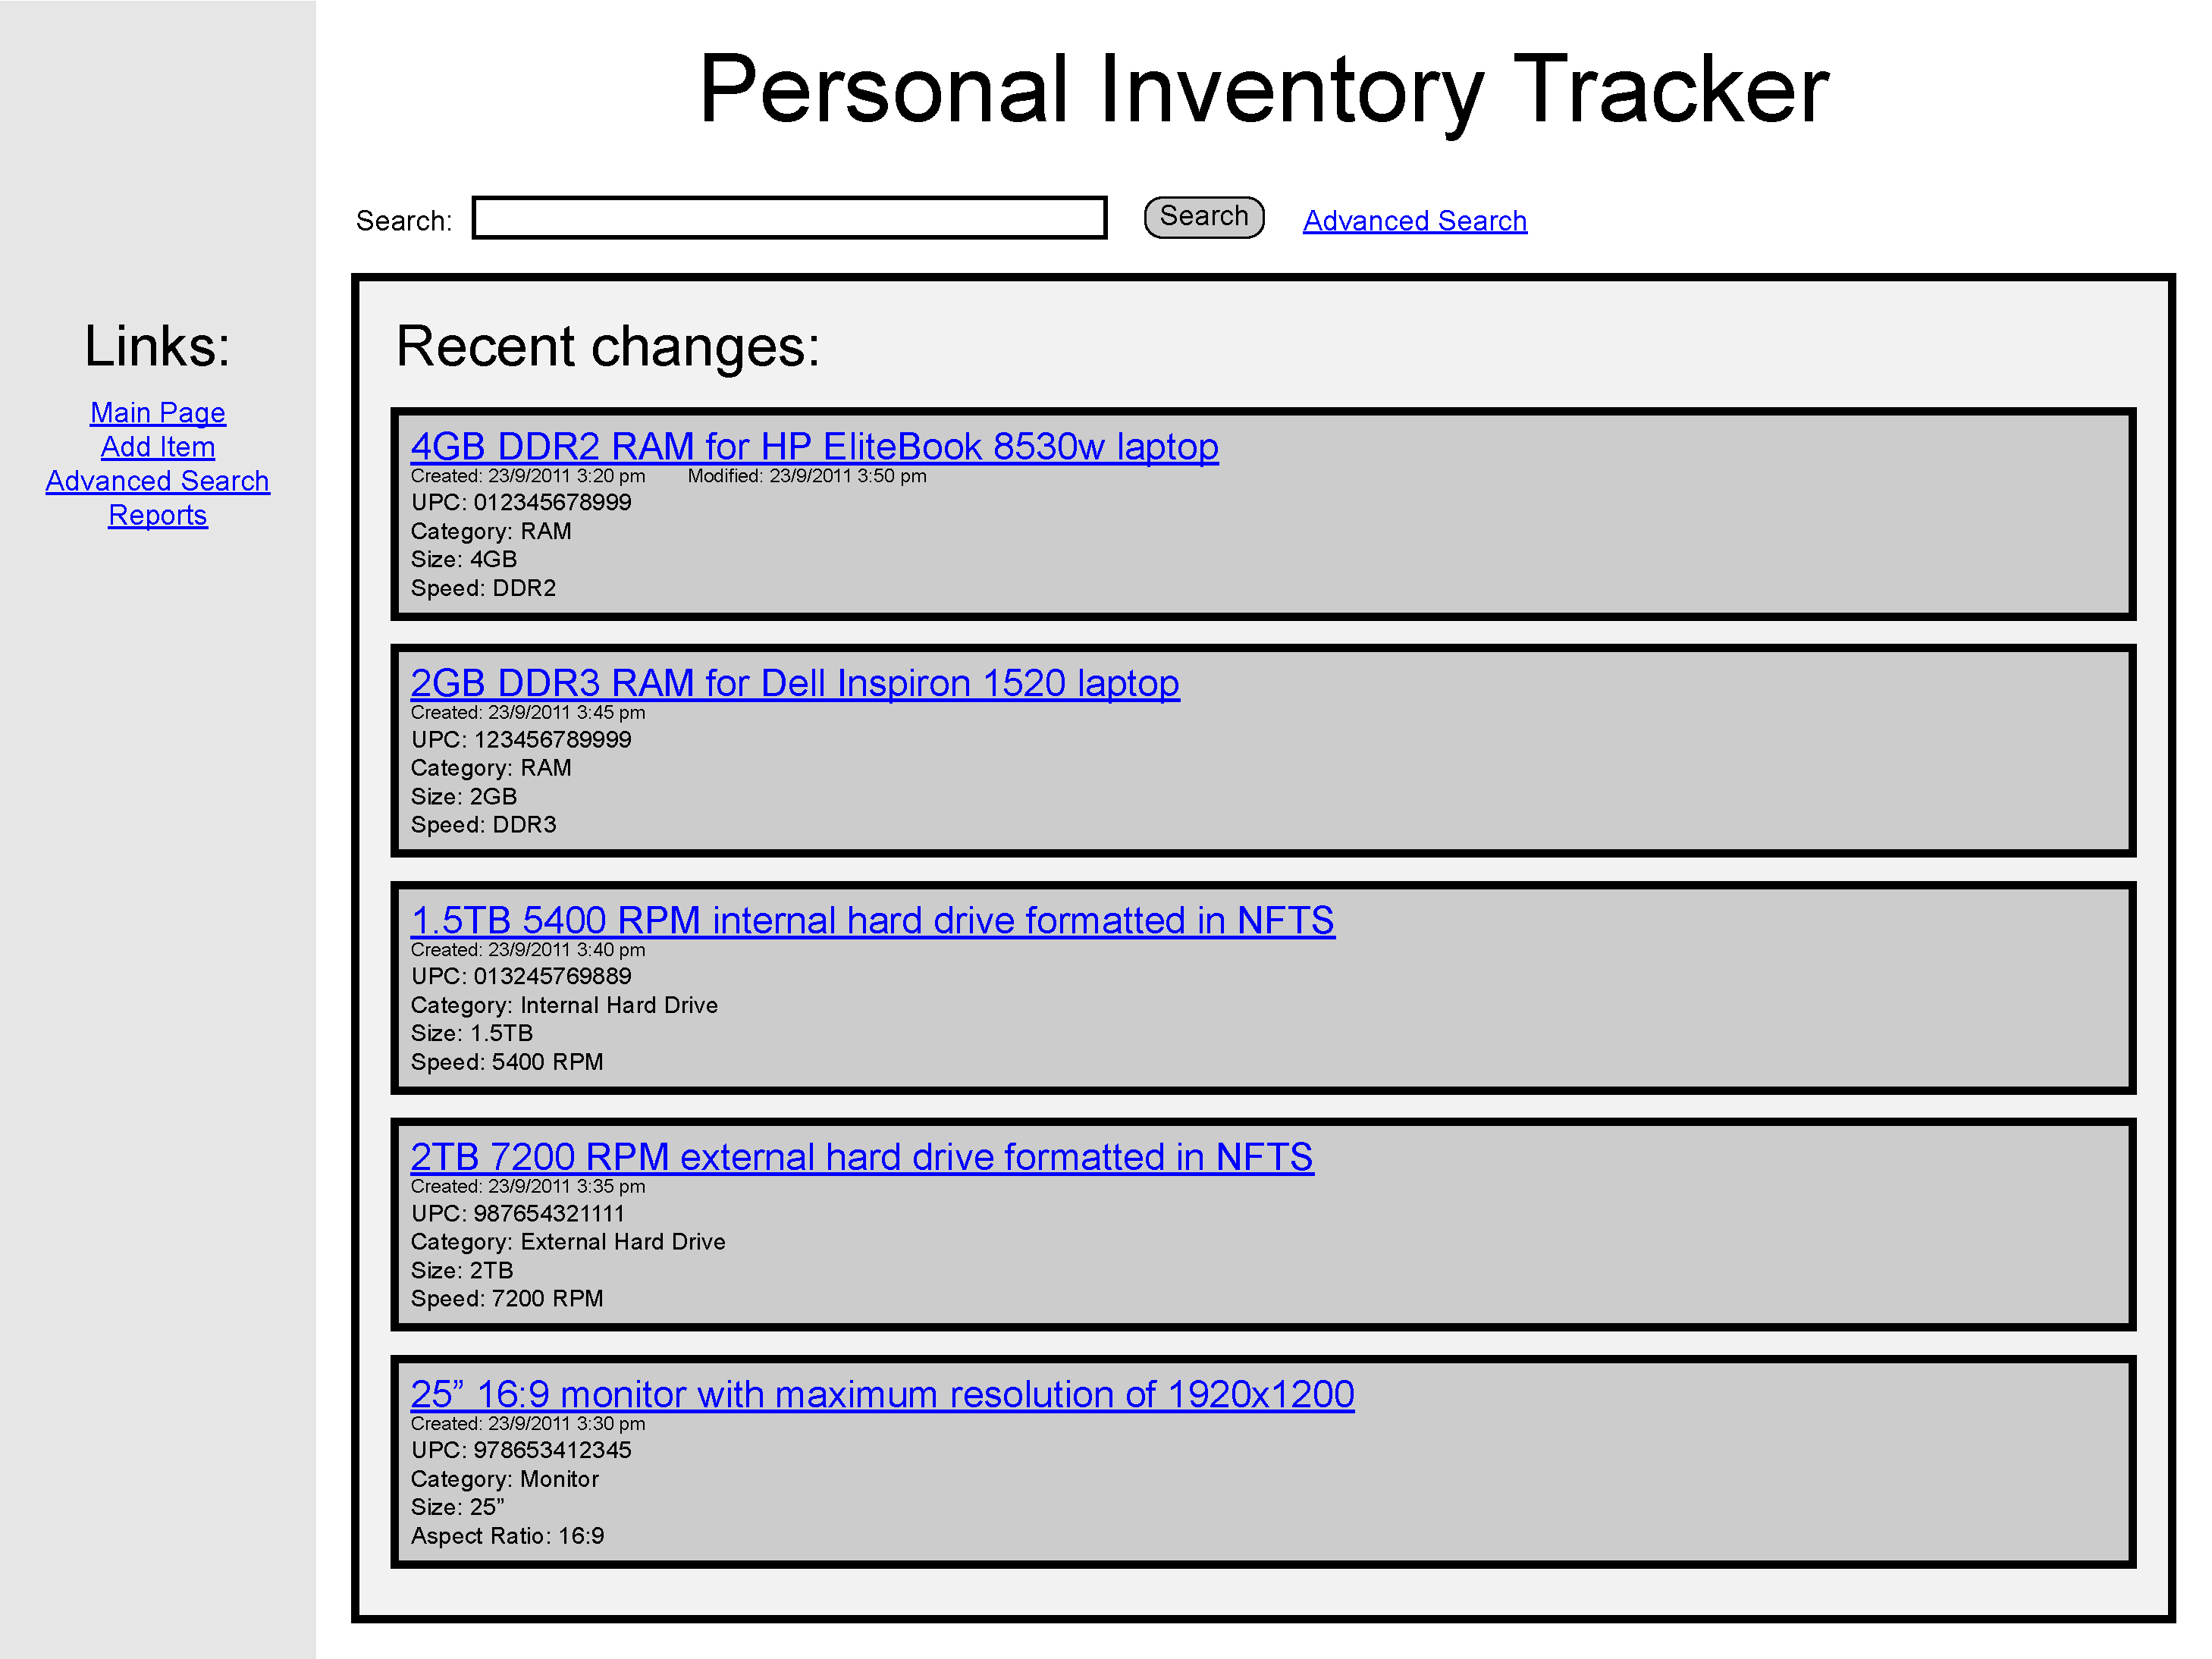
\includegraphics[keepaspectratio, width=4.5in]{addItemF0S0.pdf}\\
The main page
\end{tabular}\\
~\\
~\\
\begin{tabular}{ p{4.5in} }
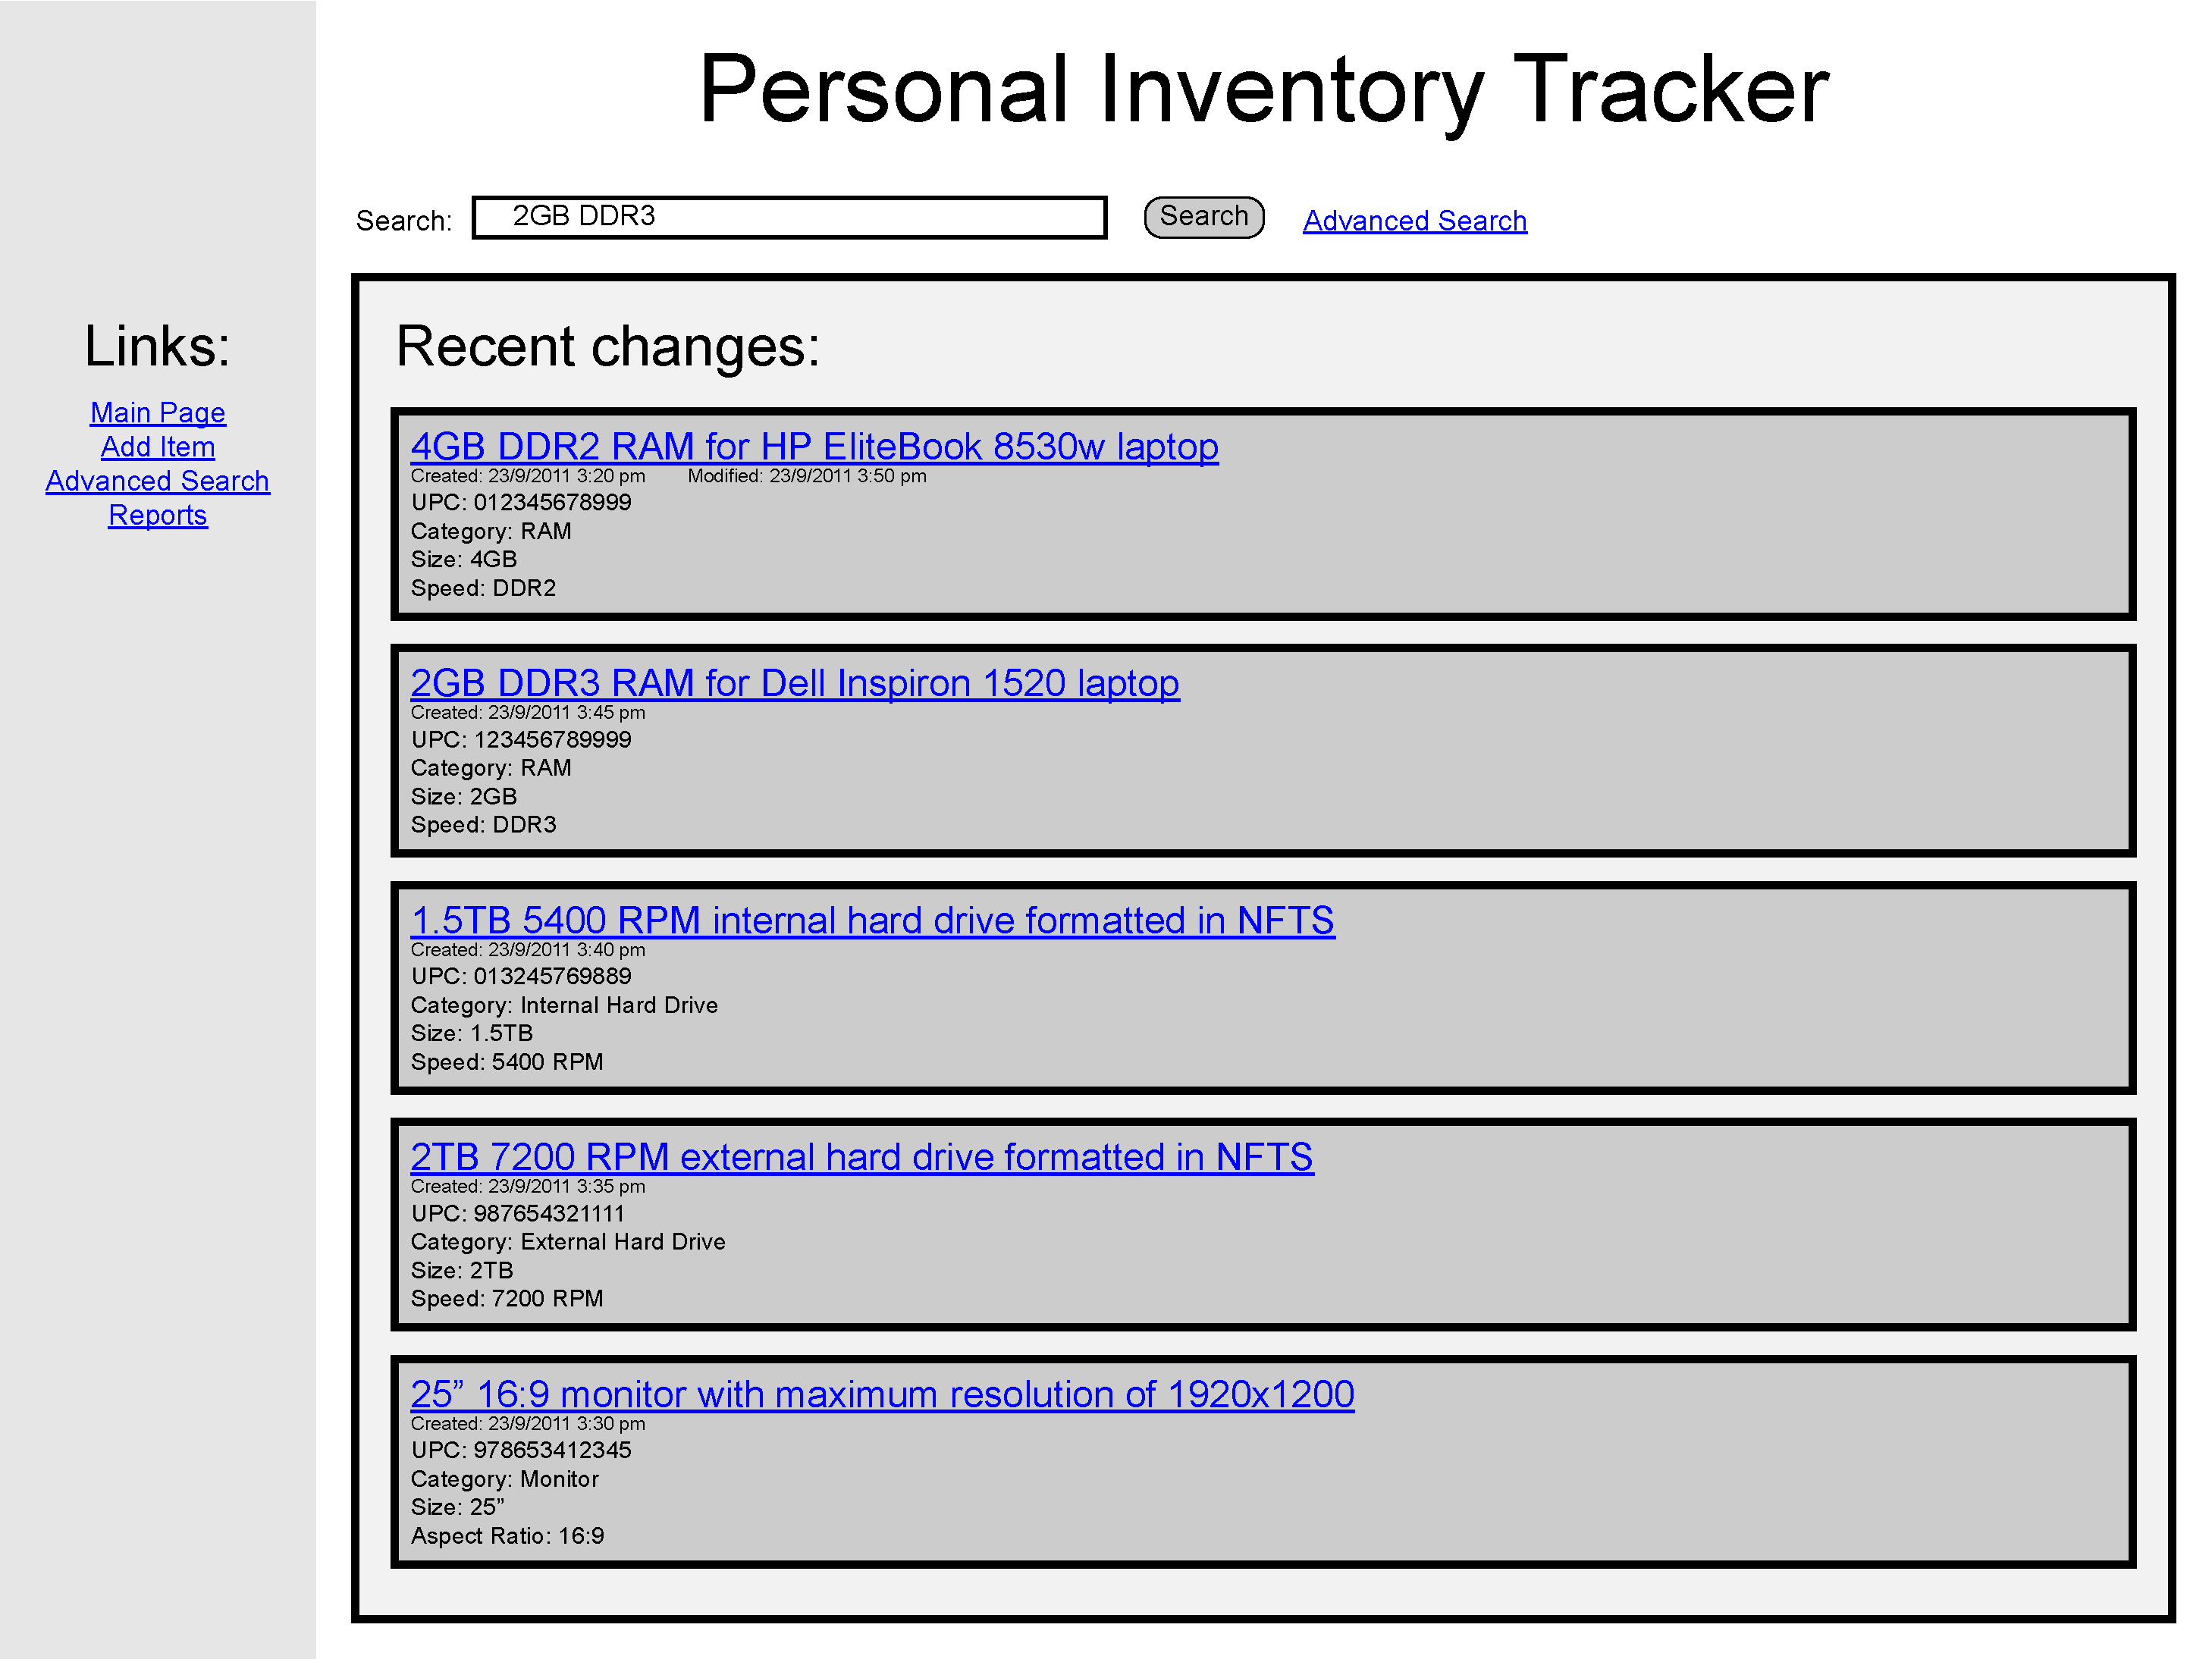
\includegraphics[keepaspectratio, width=4.5in]{basicSearchF0S0.pdf} \\
The main page with a basic search query filled in
\end{tabular}\\
~\\
~\\
\begin{tabular}{ p{4.5in} }
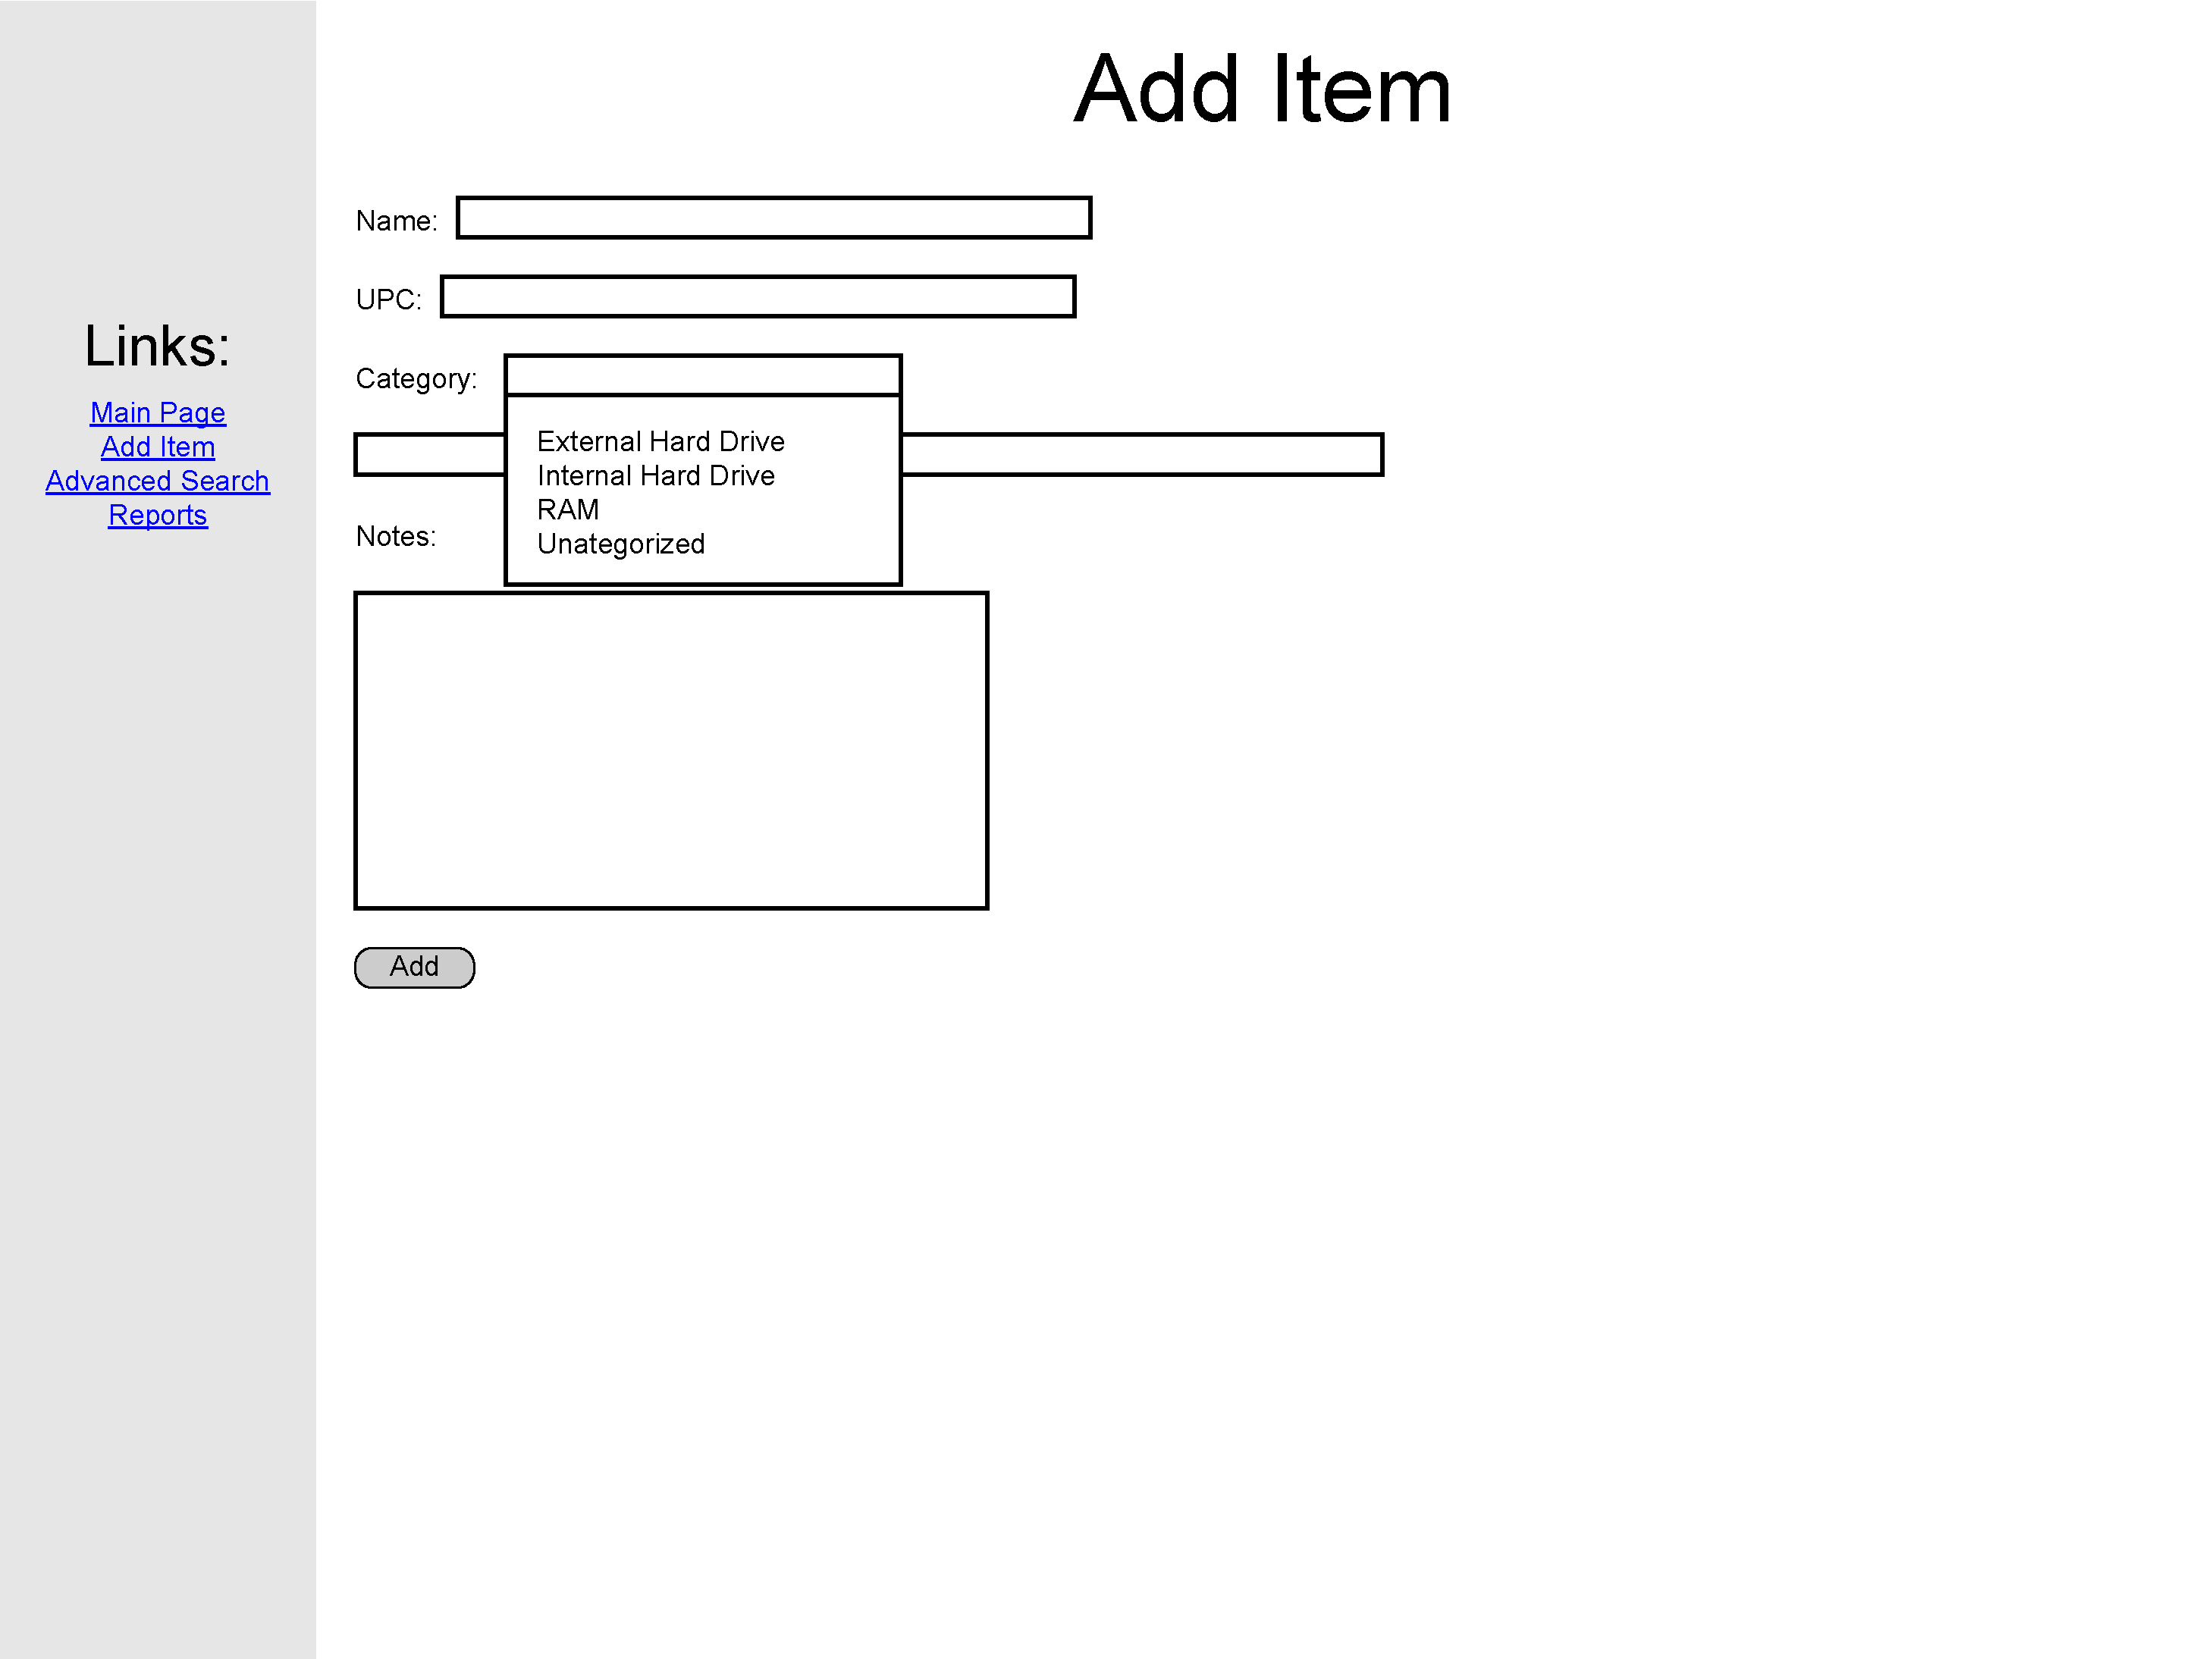
\includegraphics[keepaspectratio, width=4.5in]{addItemF0S1.pdf}\\
The add item page with category autocomplete showing
\end{tabular}\\
~\\
~\\
\begin{tabular}{ p{4.5in} }
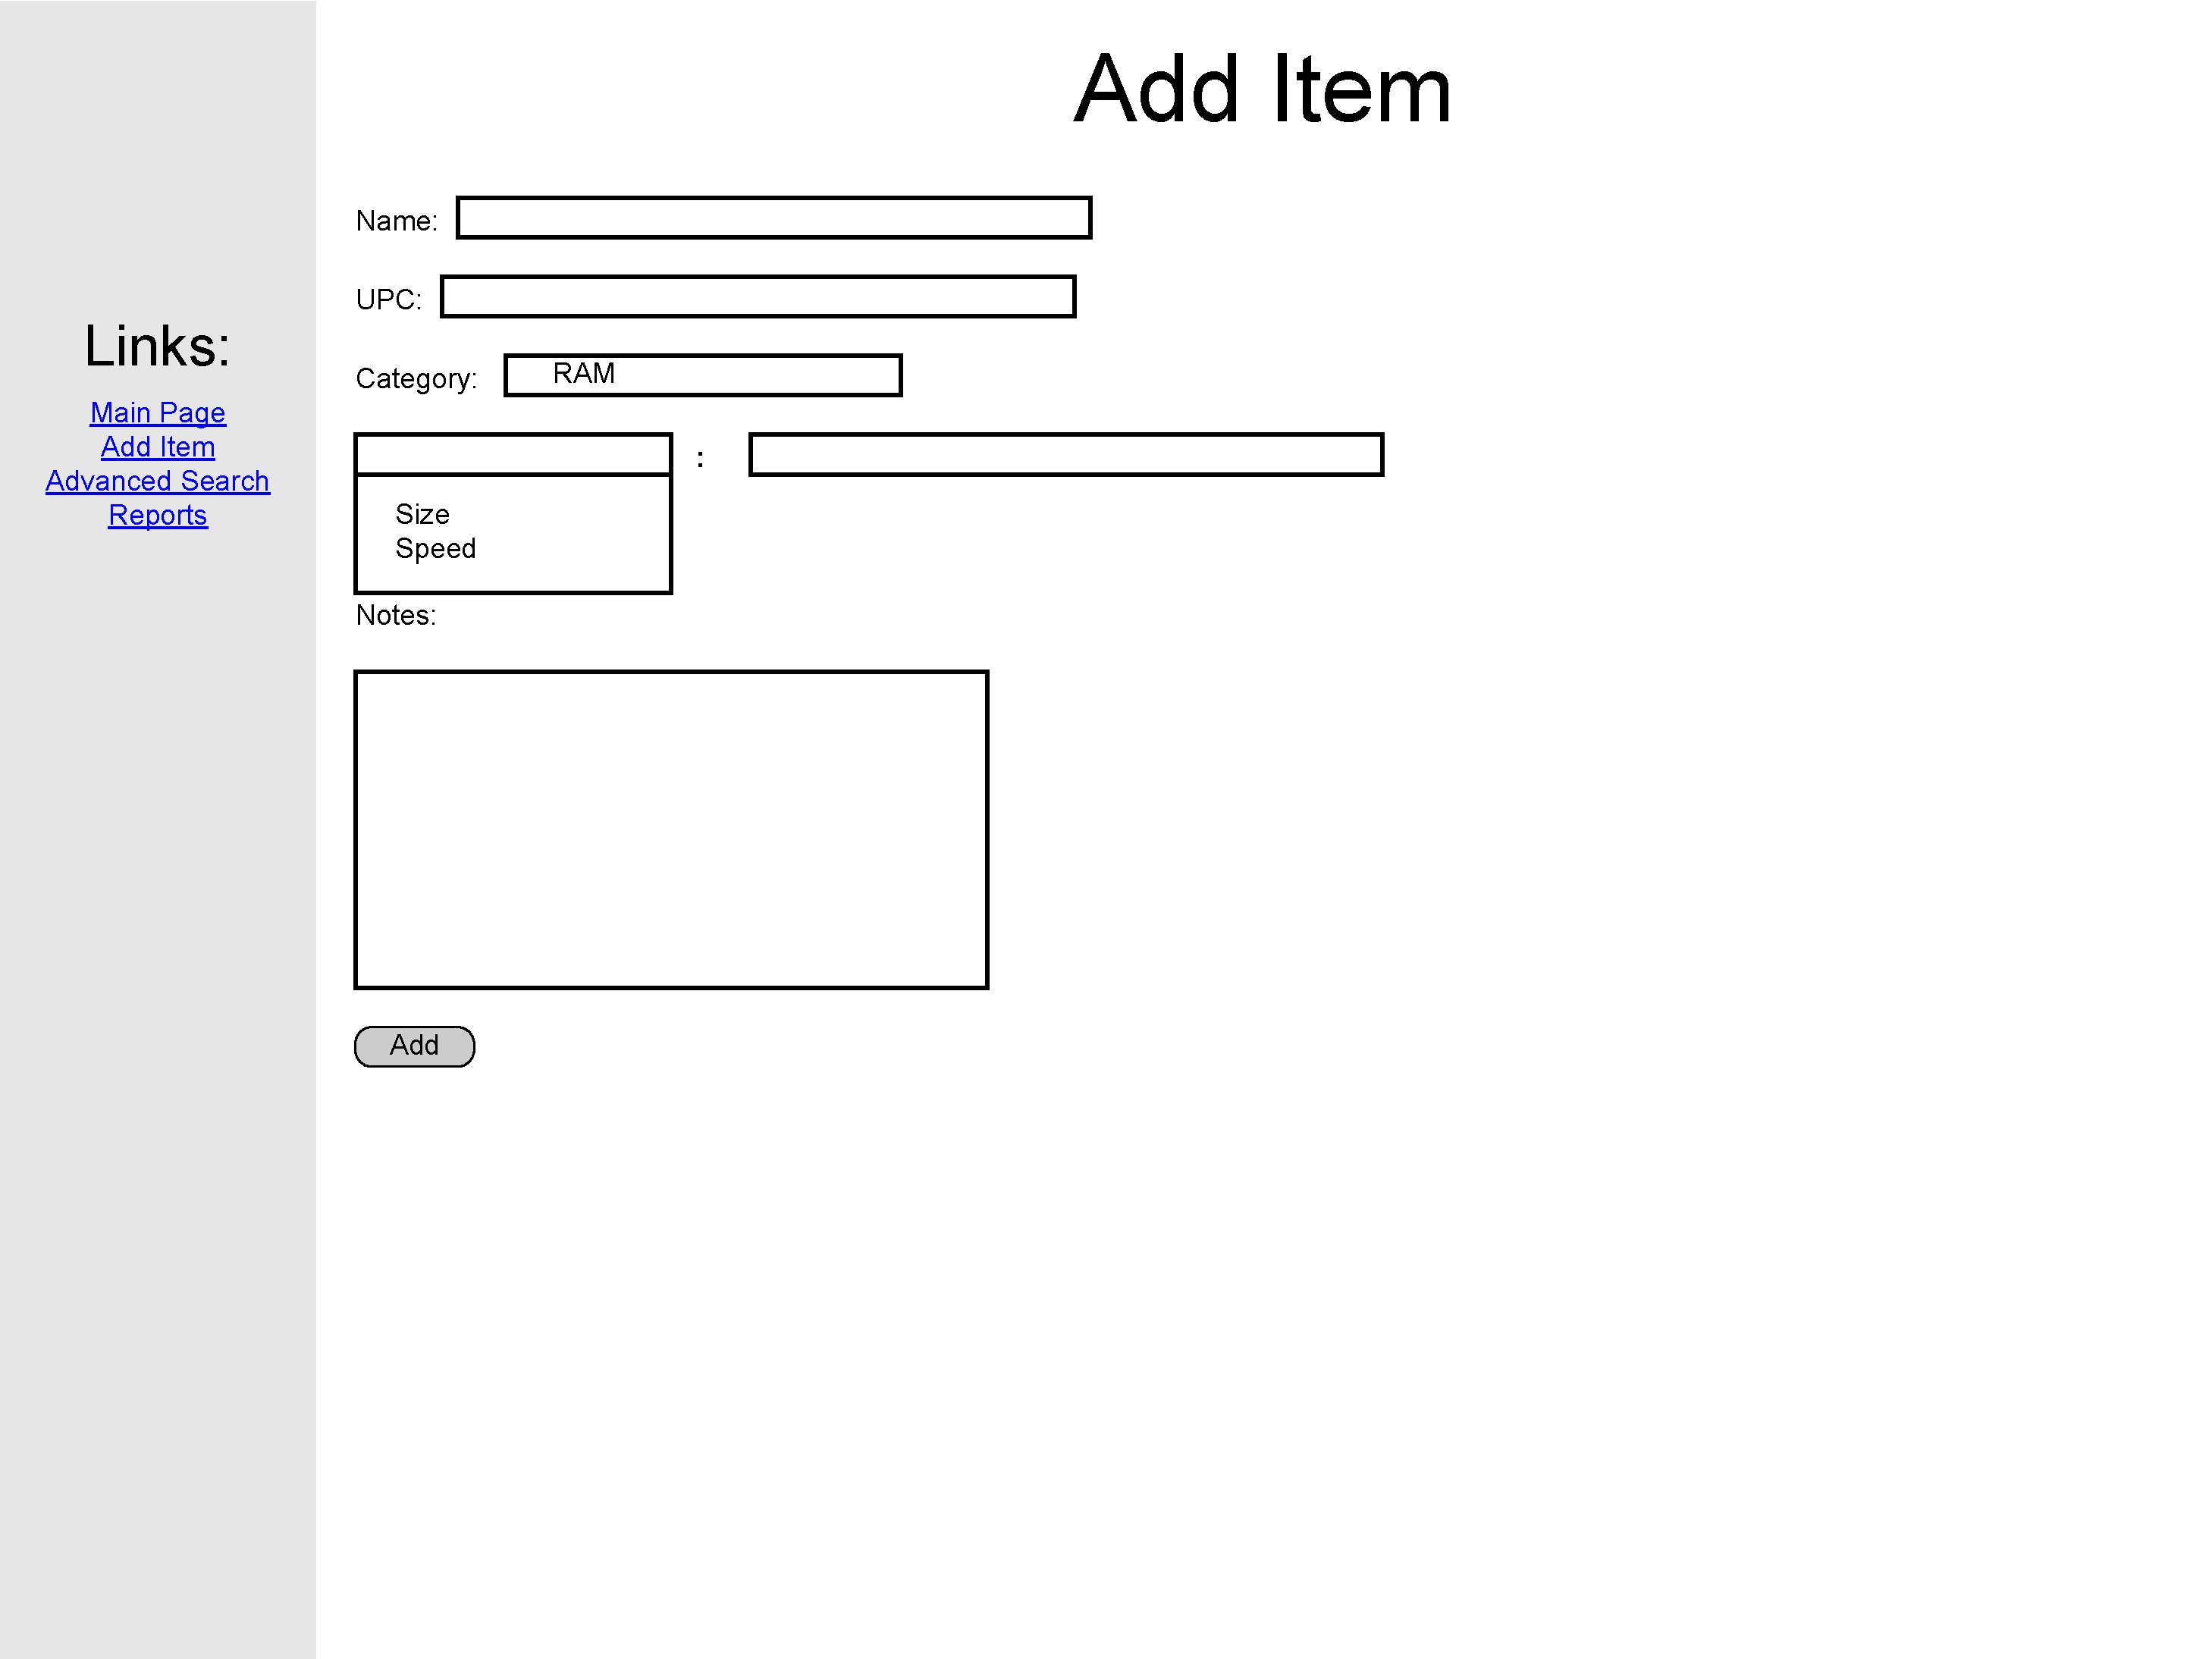
\includegraphics[keepaspectratio, width=4.5in]{addItemF0S2.pdf}  \\
The add item page with category selected and attribute autocomplete showing
\end{tabular}\\
~\\
~\\
\begin{tabular}{ p{4.5in} }
\includegraphics[keepaspectratio, width=4.5in]{addItemF0S3.pdf}\\
The add item page after one attribute key has been selected and another field added
\end{tabular}\\
~\\
~\\
\begin{tabular}{ p{4.5in} }
\includegraphics[keepaspectratio, width=4.5in]{addItemF0S5.pdf}\\
The add item page with data filled in
\end{tabular}\\
~\\
~\\
\begin{tabular}{ p{4.5in} }
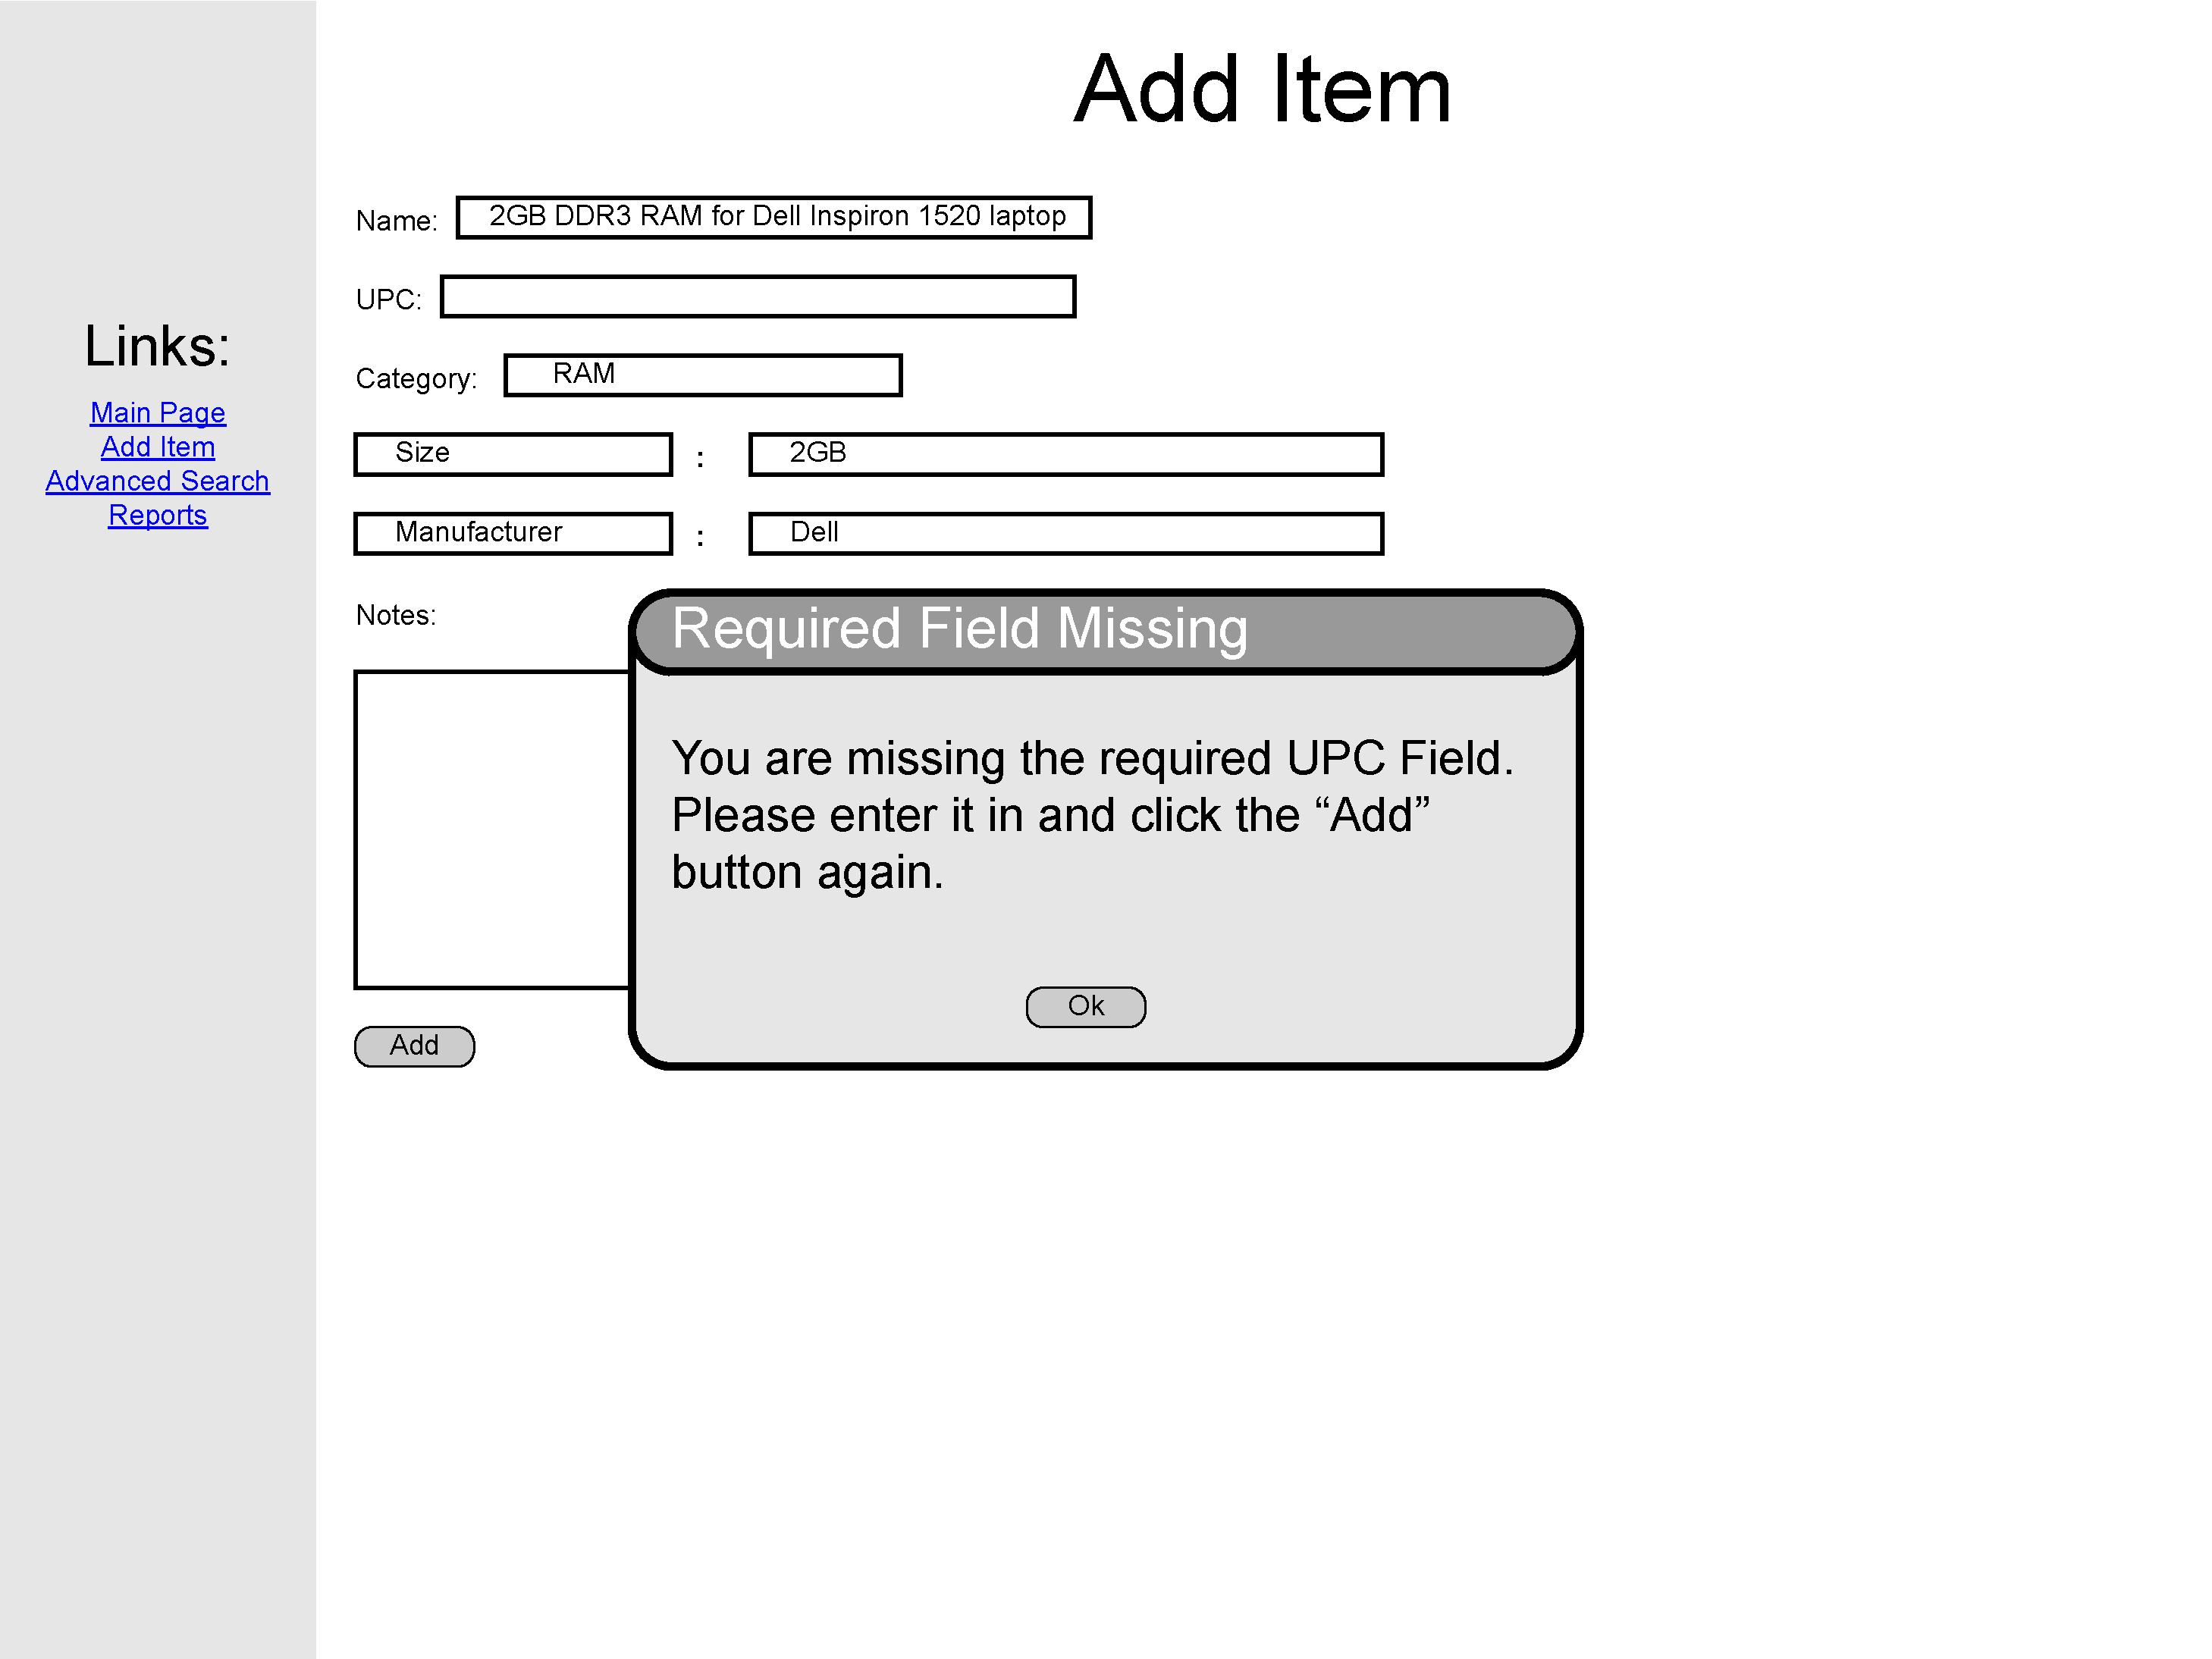
\includegraphics[keepaspectratio, width=4.5in]{addItemF1S5.pdf} \\
Popup message informing the user that the required UPC field is missing
\end{tabular}\\
~\\
~\\
\begin{tabular}{ p{4.5in} }
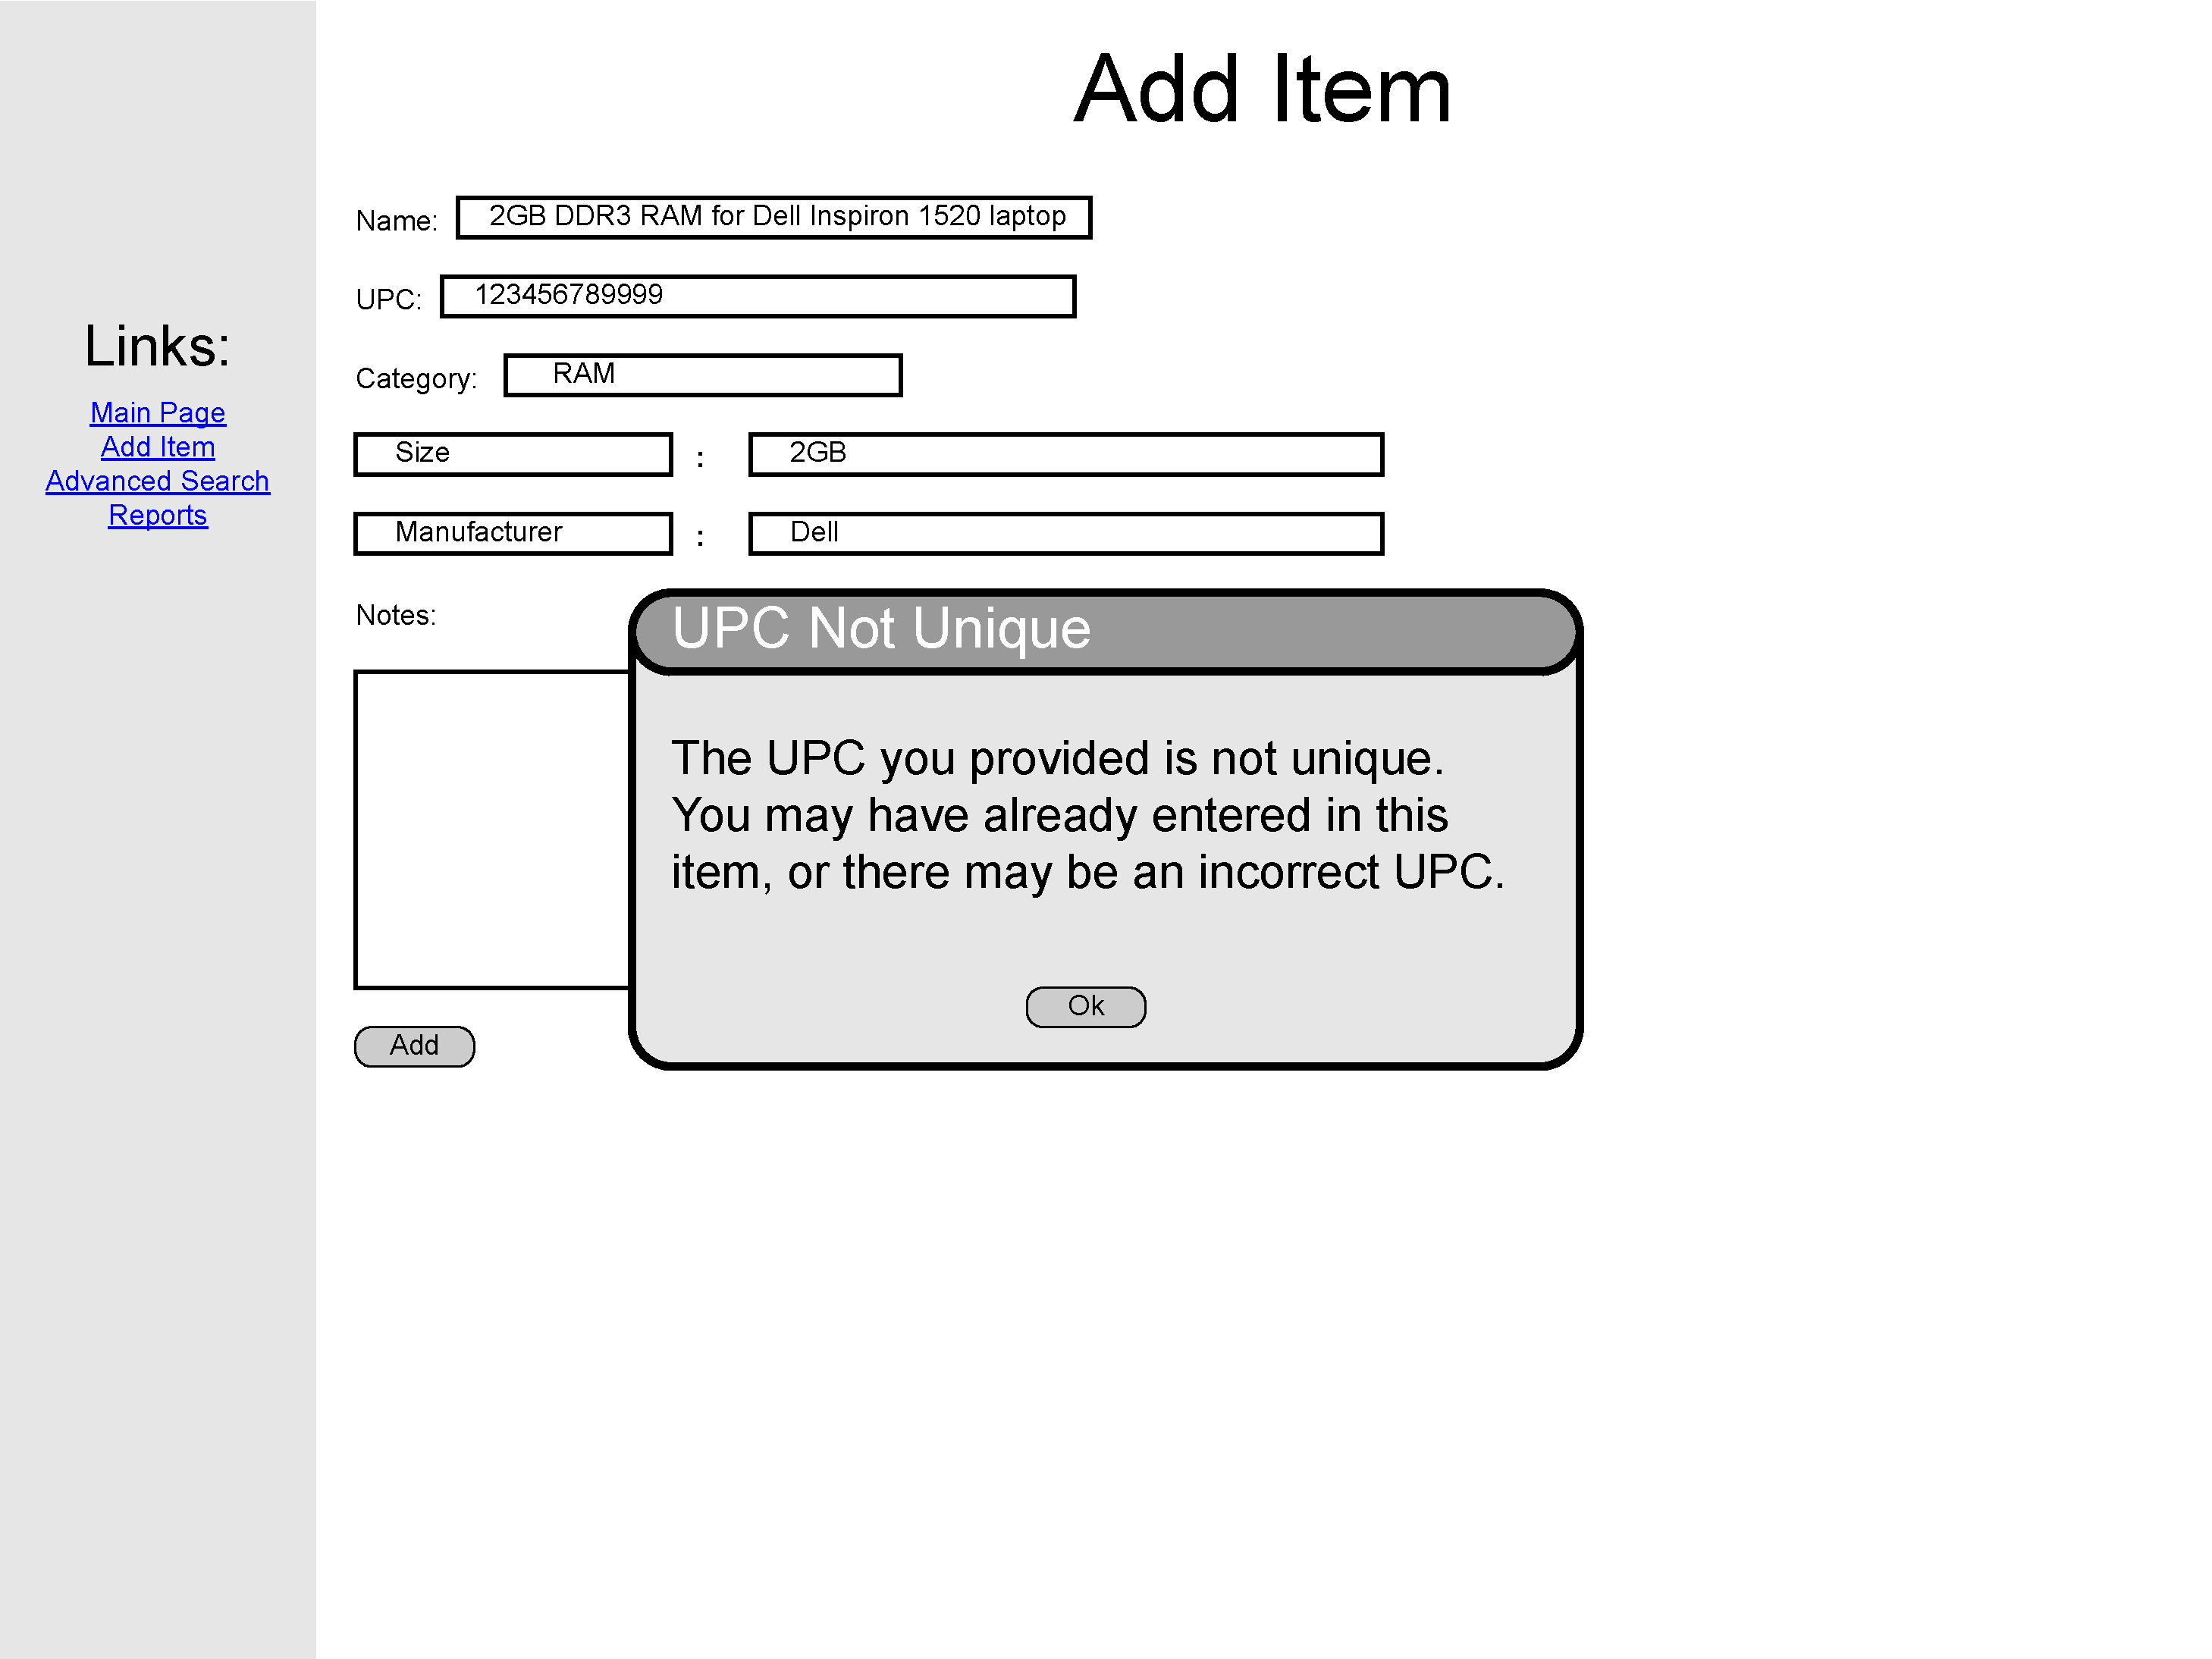
\includegraphics[keepaspectratio, width=4.5in]{addItemF2S5.pdf} \\
Popup message informing the user that the UPC entered has been previously entered
\end{tabular}
~\\
~\\
\begin{tabular}{ p{4.5in} }
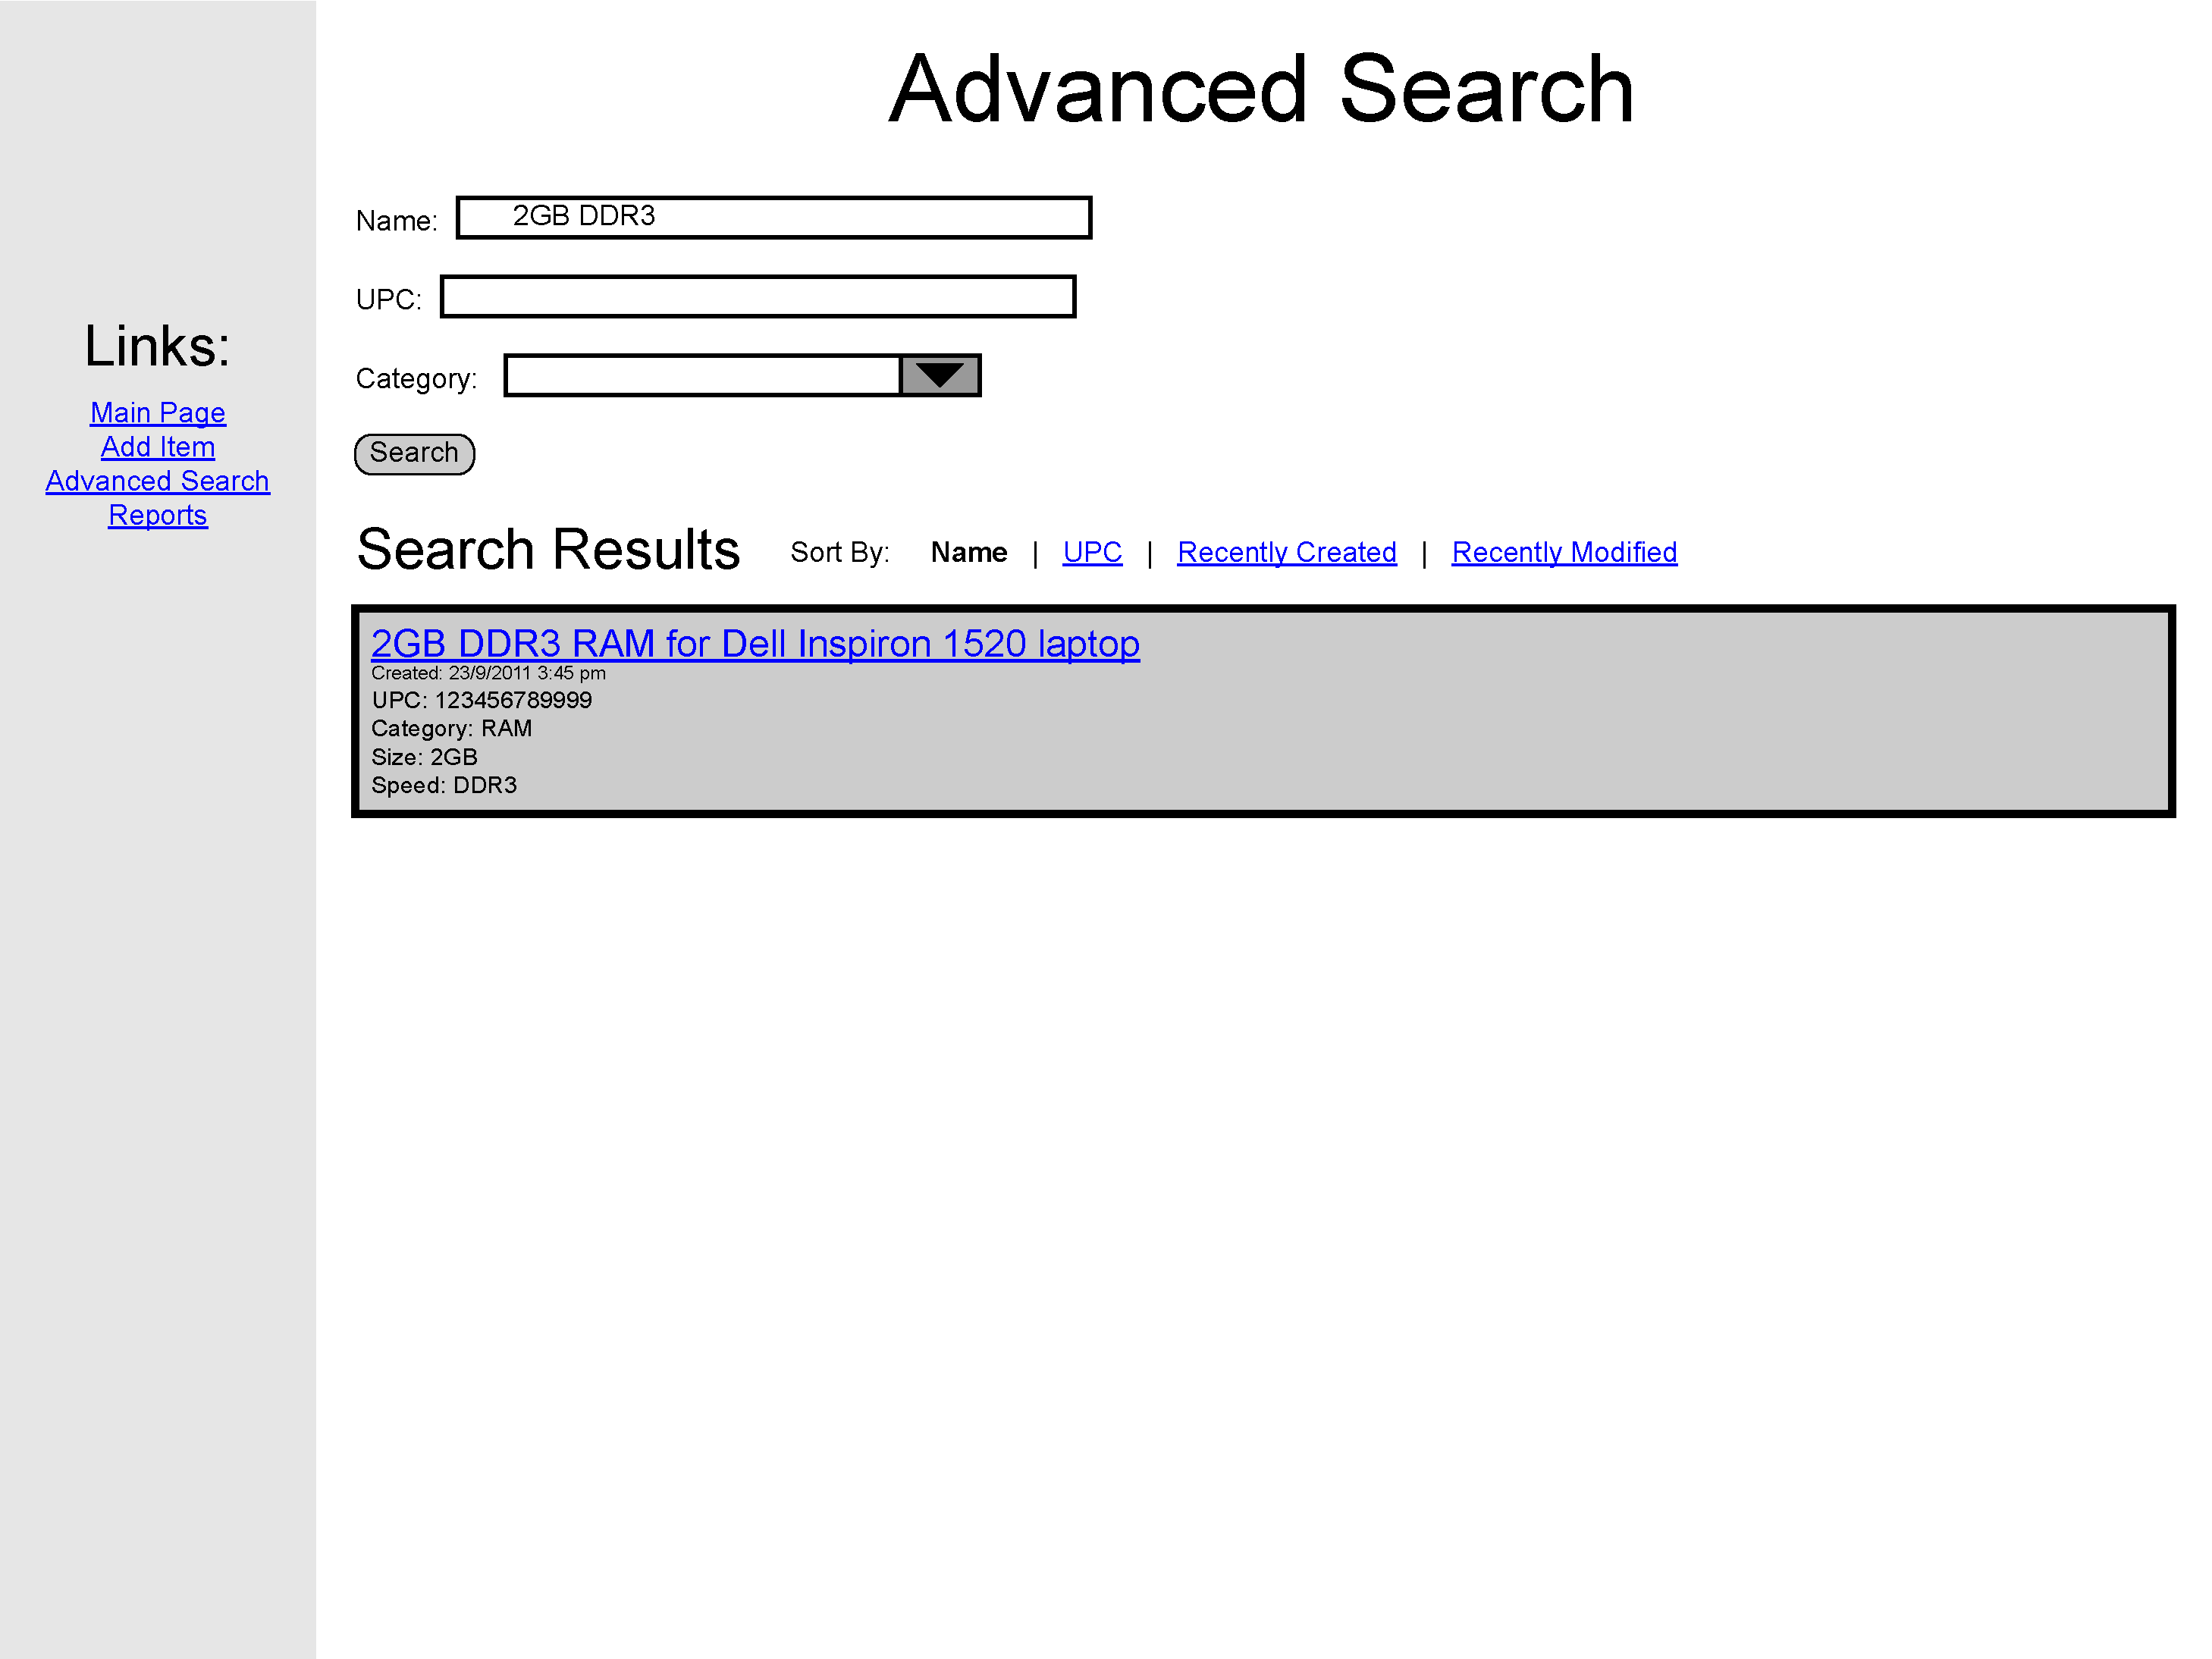
\includegraphics[keepaspectratio, width=4.5in]{basicSearchF0S1.pdf} \\
The results of the basic search
\end{tabular}\\
~\\
~\\
\begin{tabular}{ p{4.5in} }
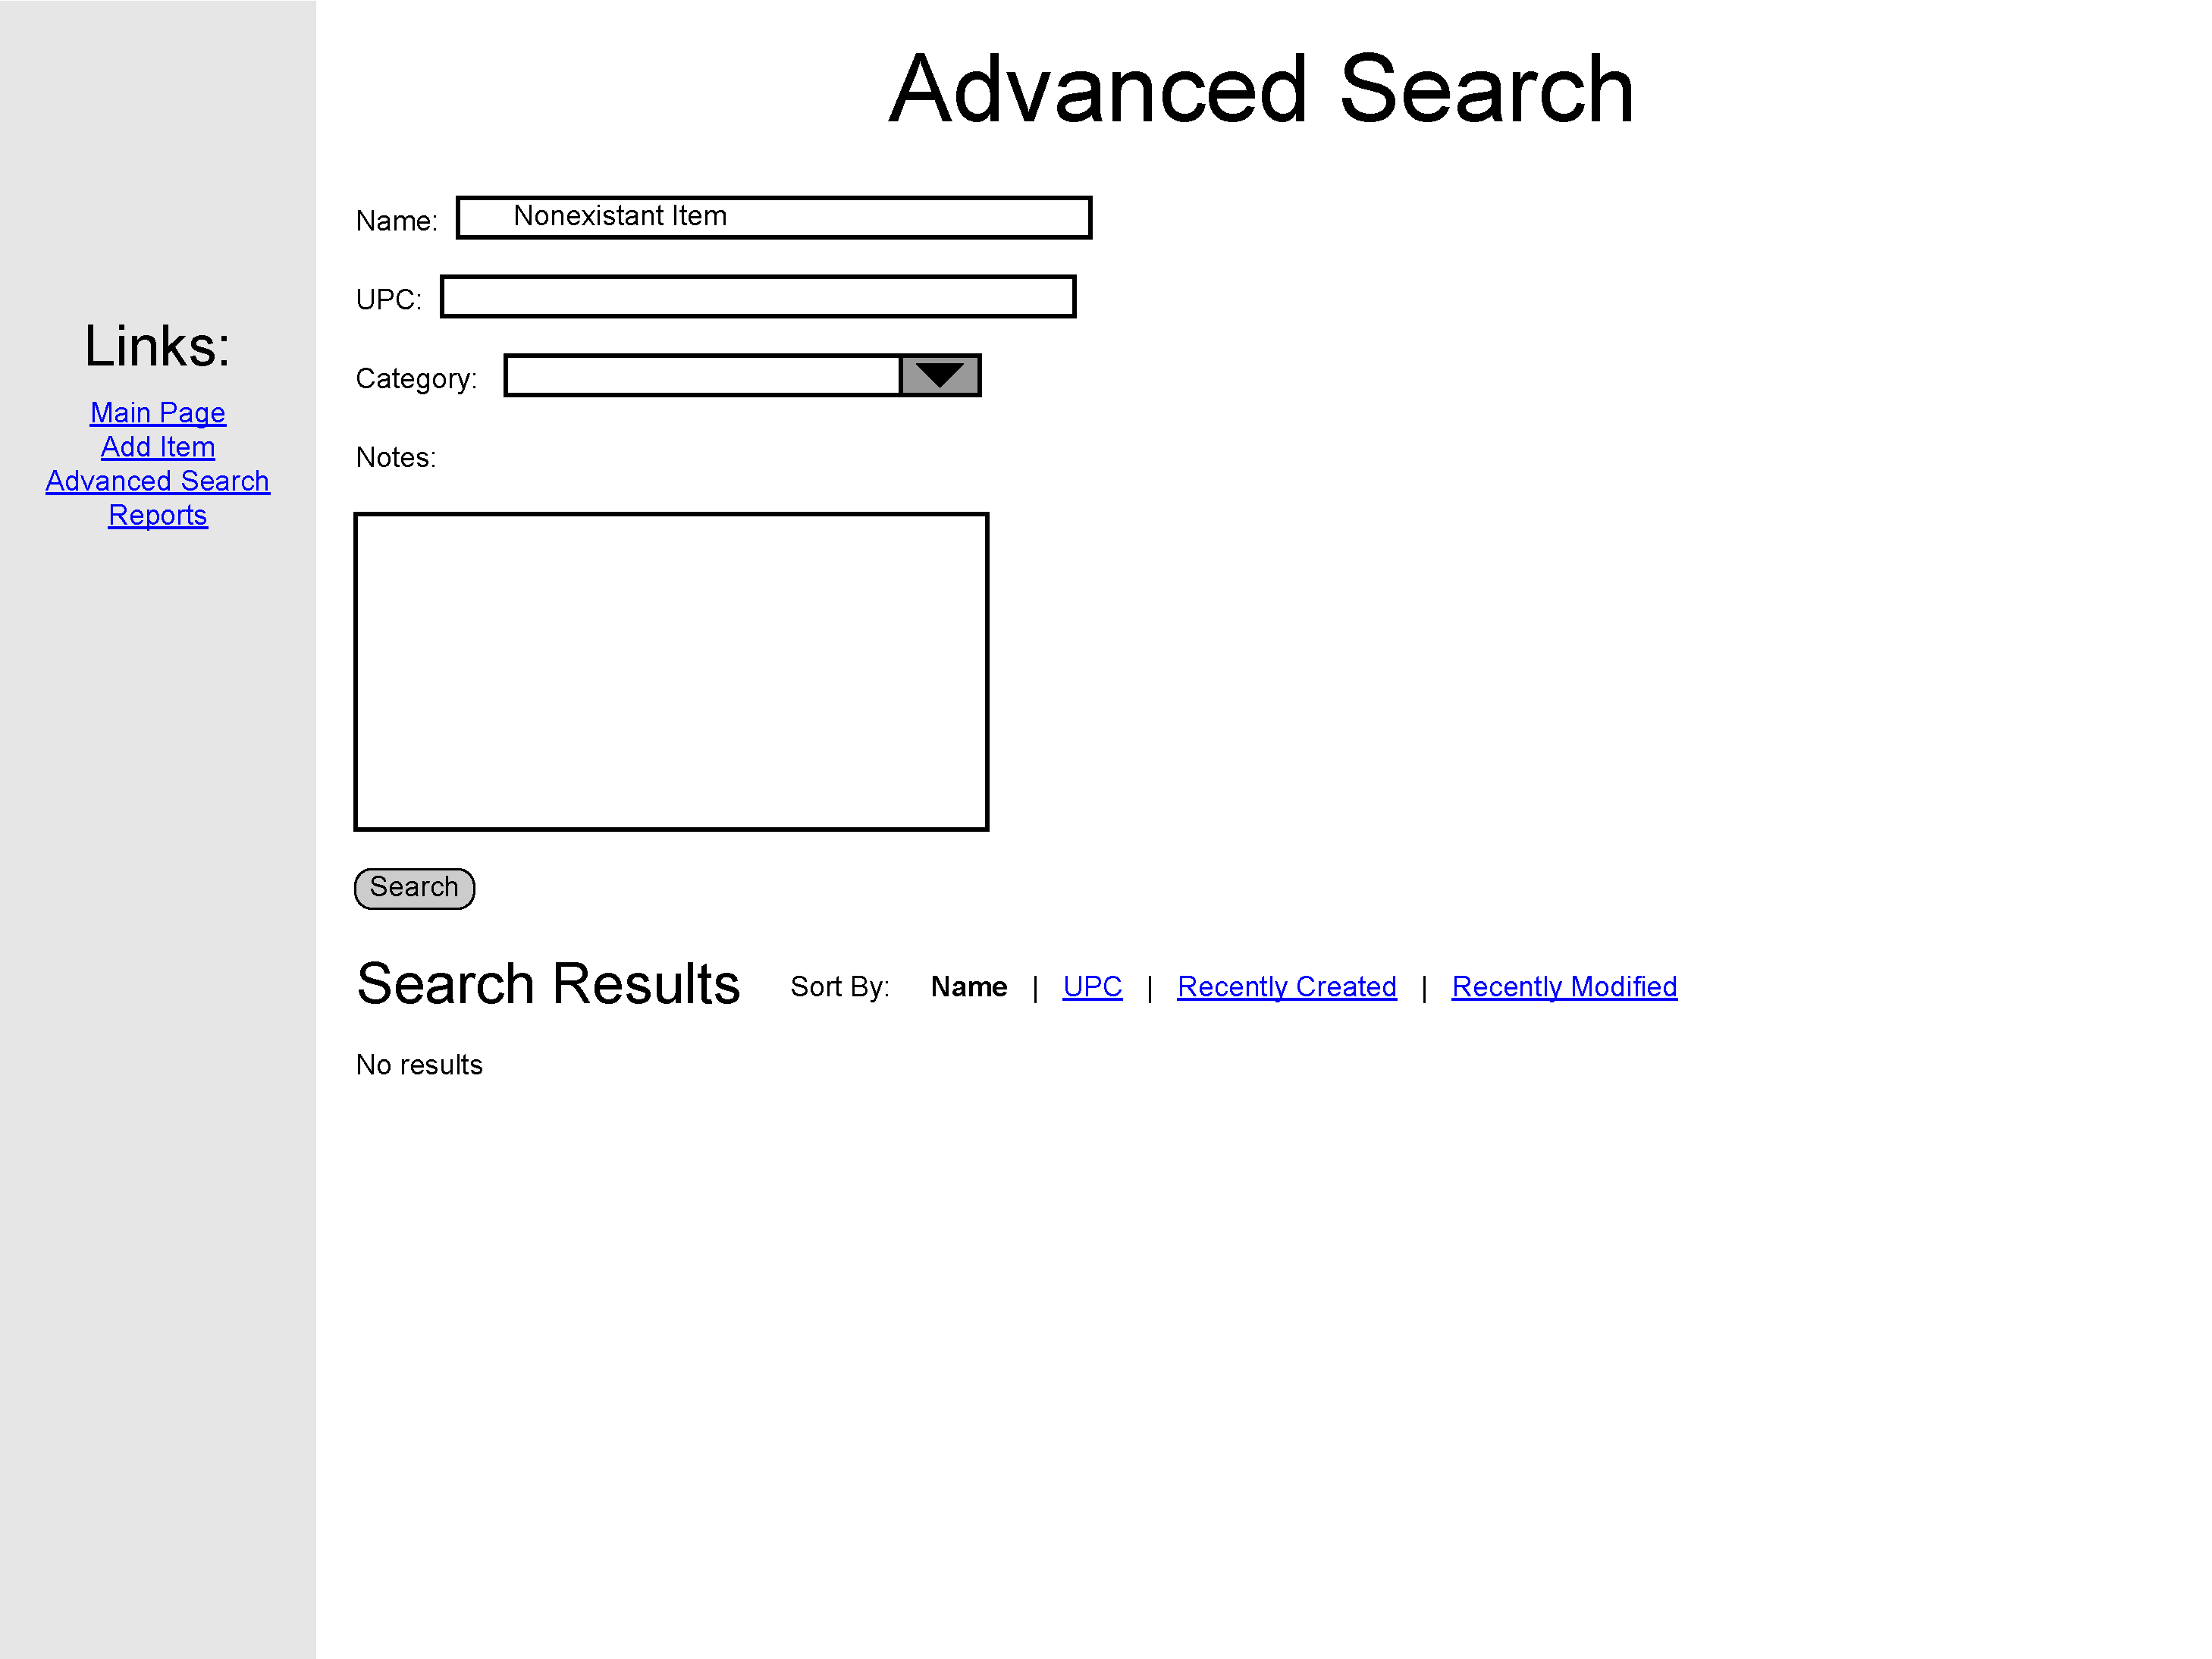
\includegraphics[keepaspectratio, width=4.5in]{basicSearchF2S1.pdf} \\
The results of the basic search when there are no matching entries
\end{tabular}
~\\
~\\
\begin{tabular}{ p{4.5in} }
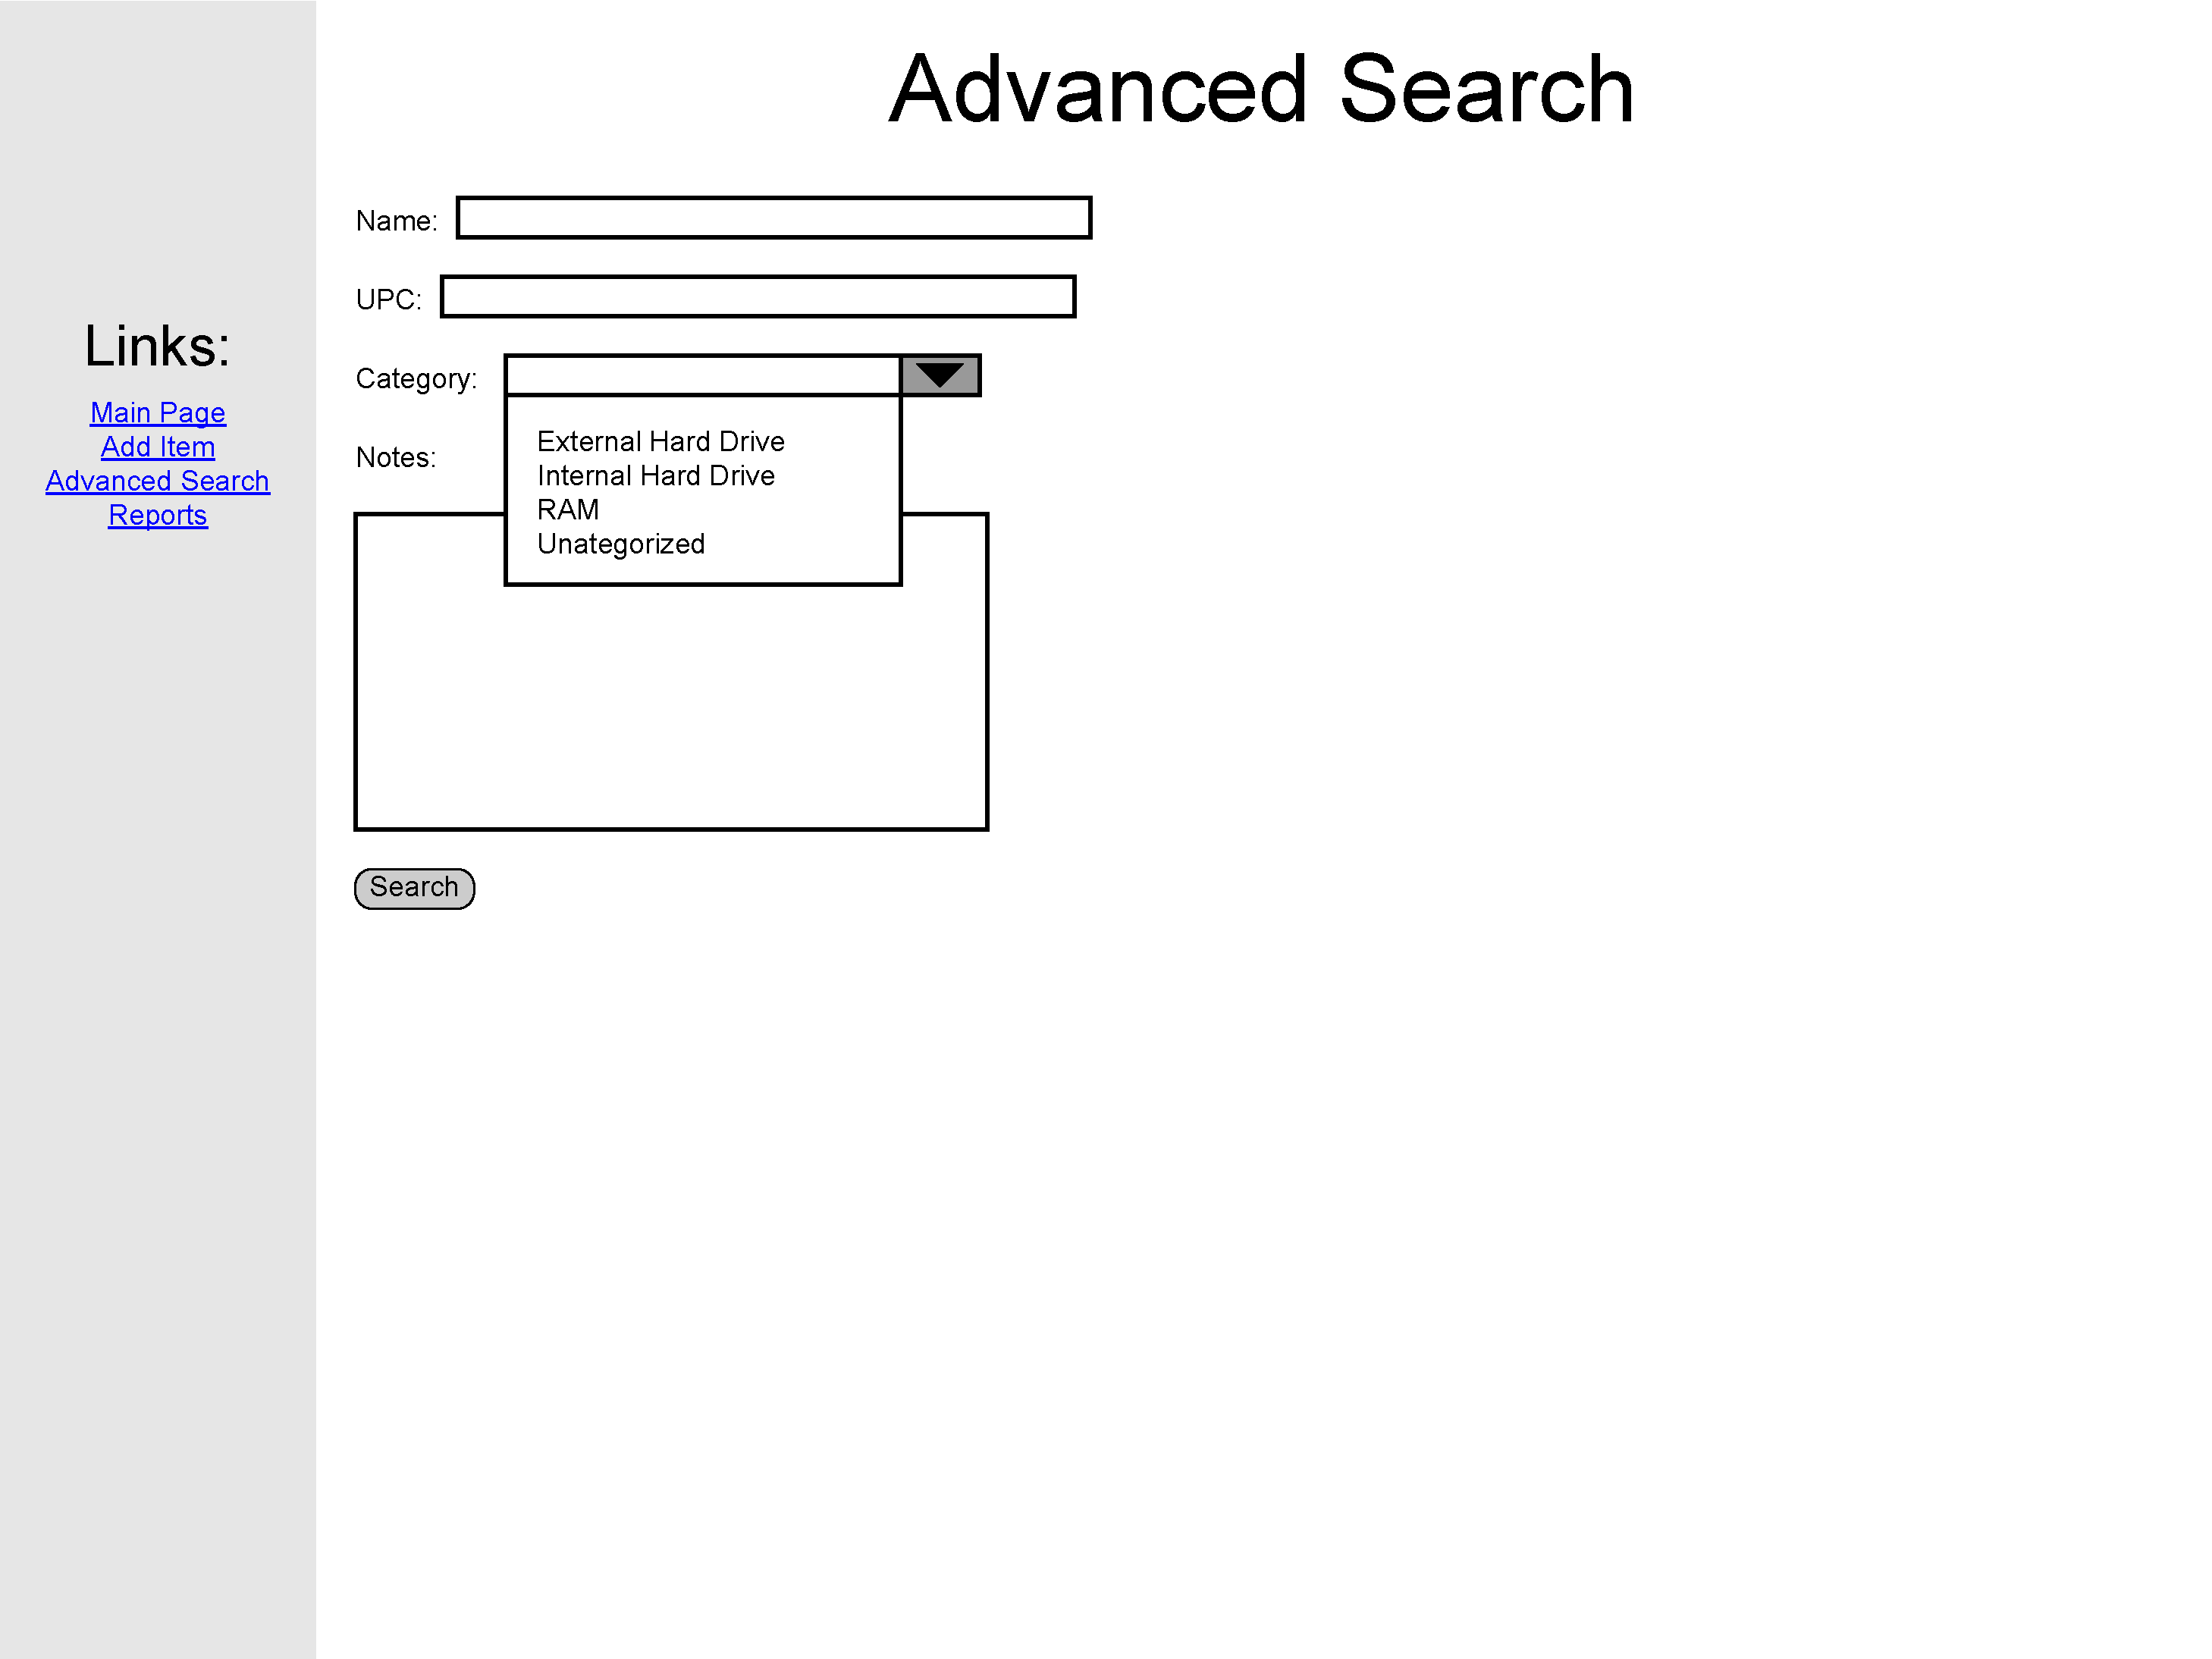
\includegraphics[keepaspectratio, width=4.5in]{advancedSearchF0S1.pdf} \\
The advanced search page with the category dropdown expanded
\end{tabular}\\
~\\
~\\
\begin{tabular}{ p{4.5in} }
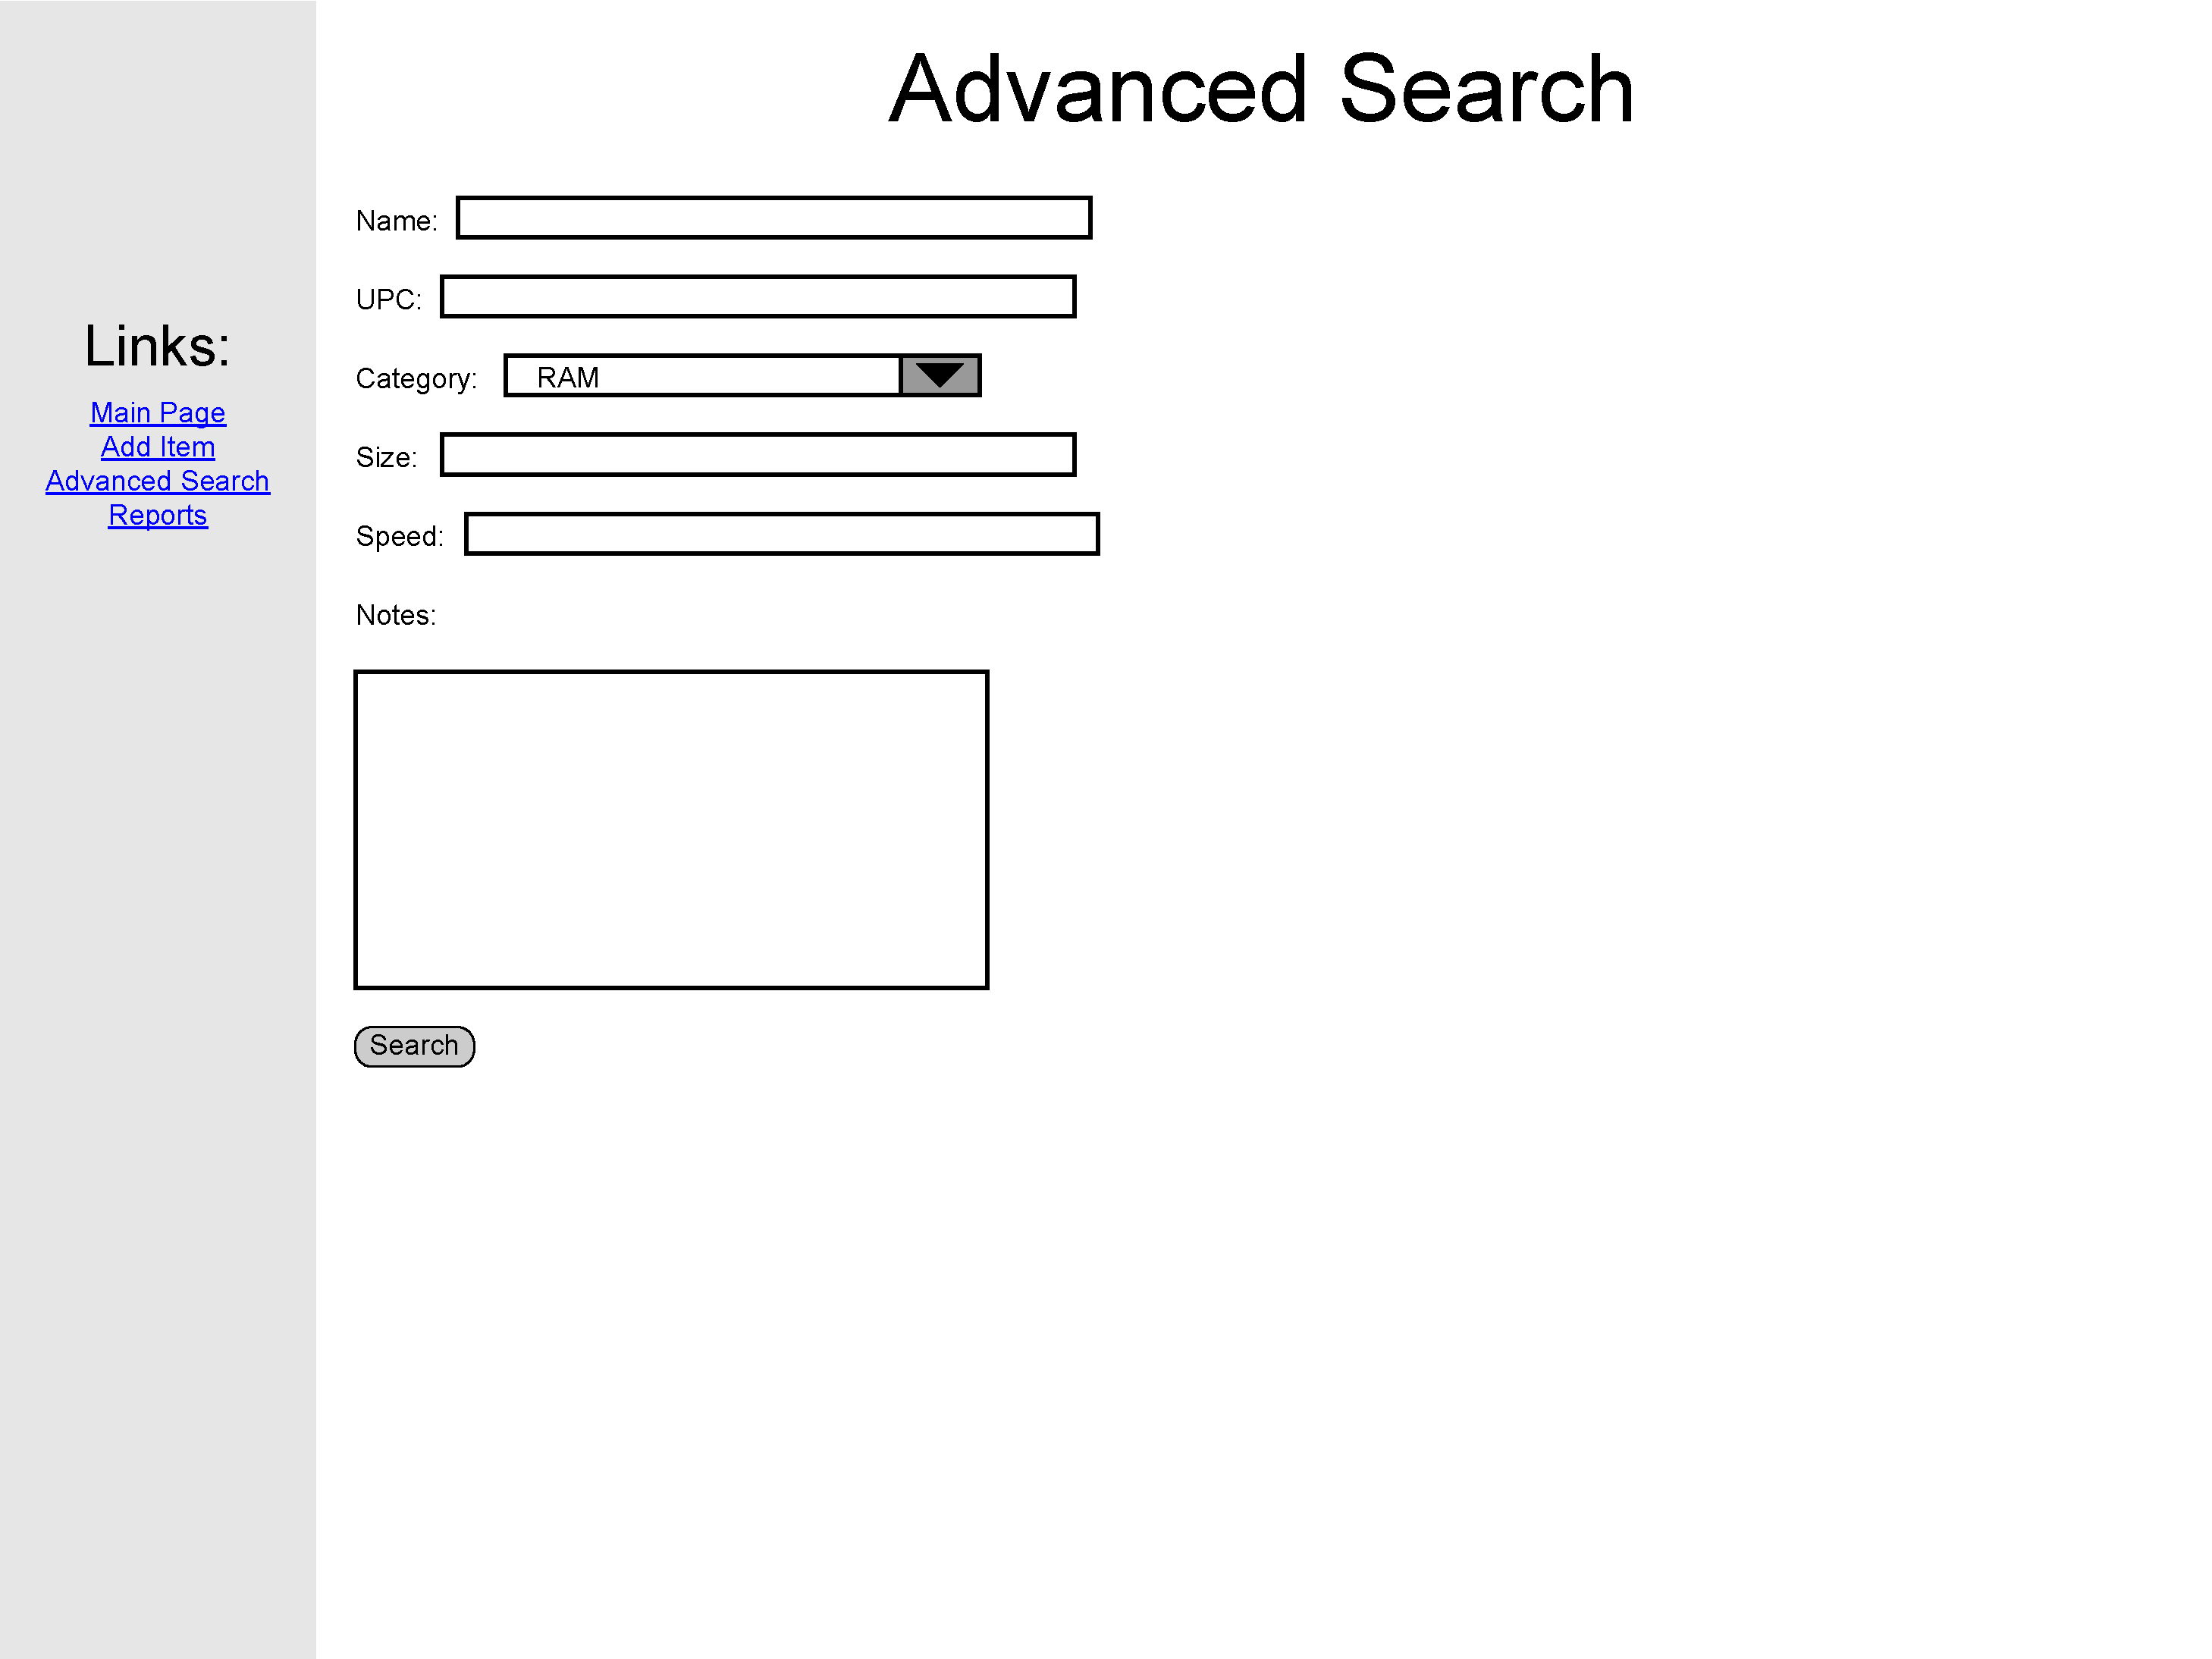
\includegraphics[keepaspectratio, width=4.5in]{advancedSearchF0S2.pdf} \\
The advanced search page with a category selected
\end{tabular}\\
~\\
~\\
\begin{tabular}{ p{4.5in} }
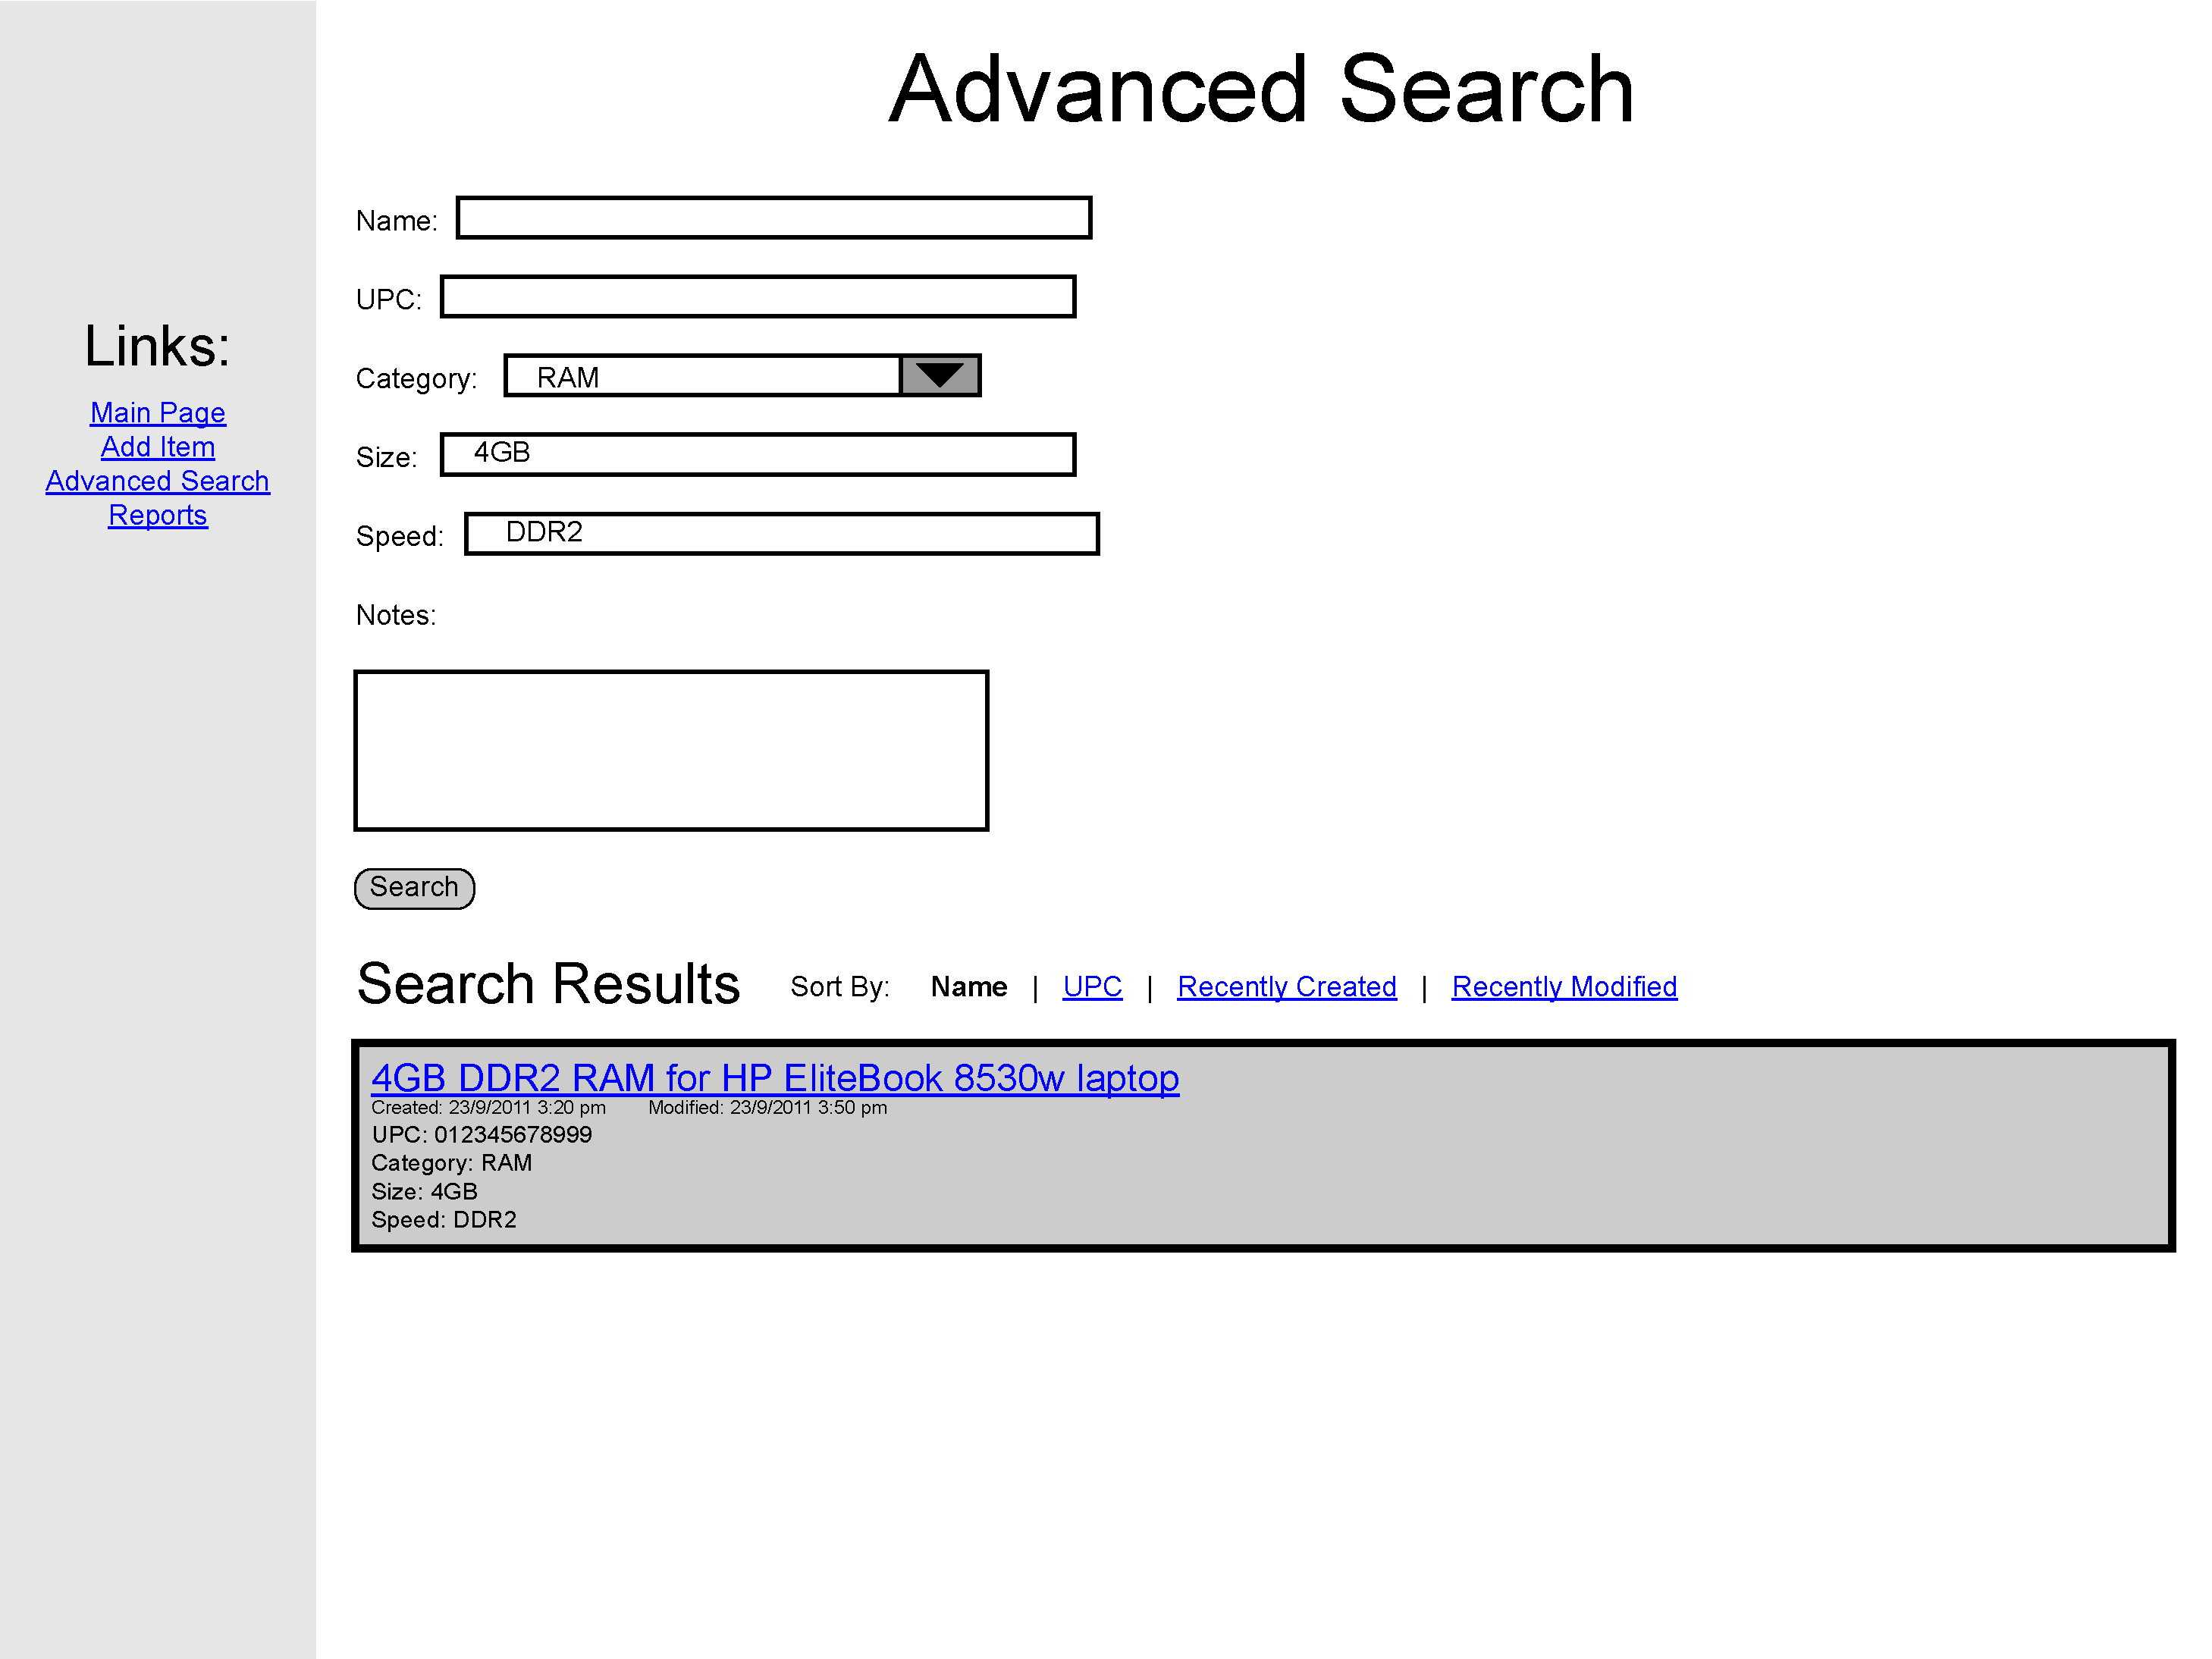
\includegraphics[keepaspectratio, width=4.5in]{advancedSearchF0S3.pdf} \\
The advanced search page with results showing
\end{tabular}\\
~\\
~\\
\begin{tabular}{ p{4.5in} }
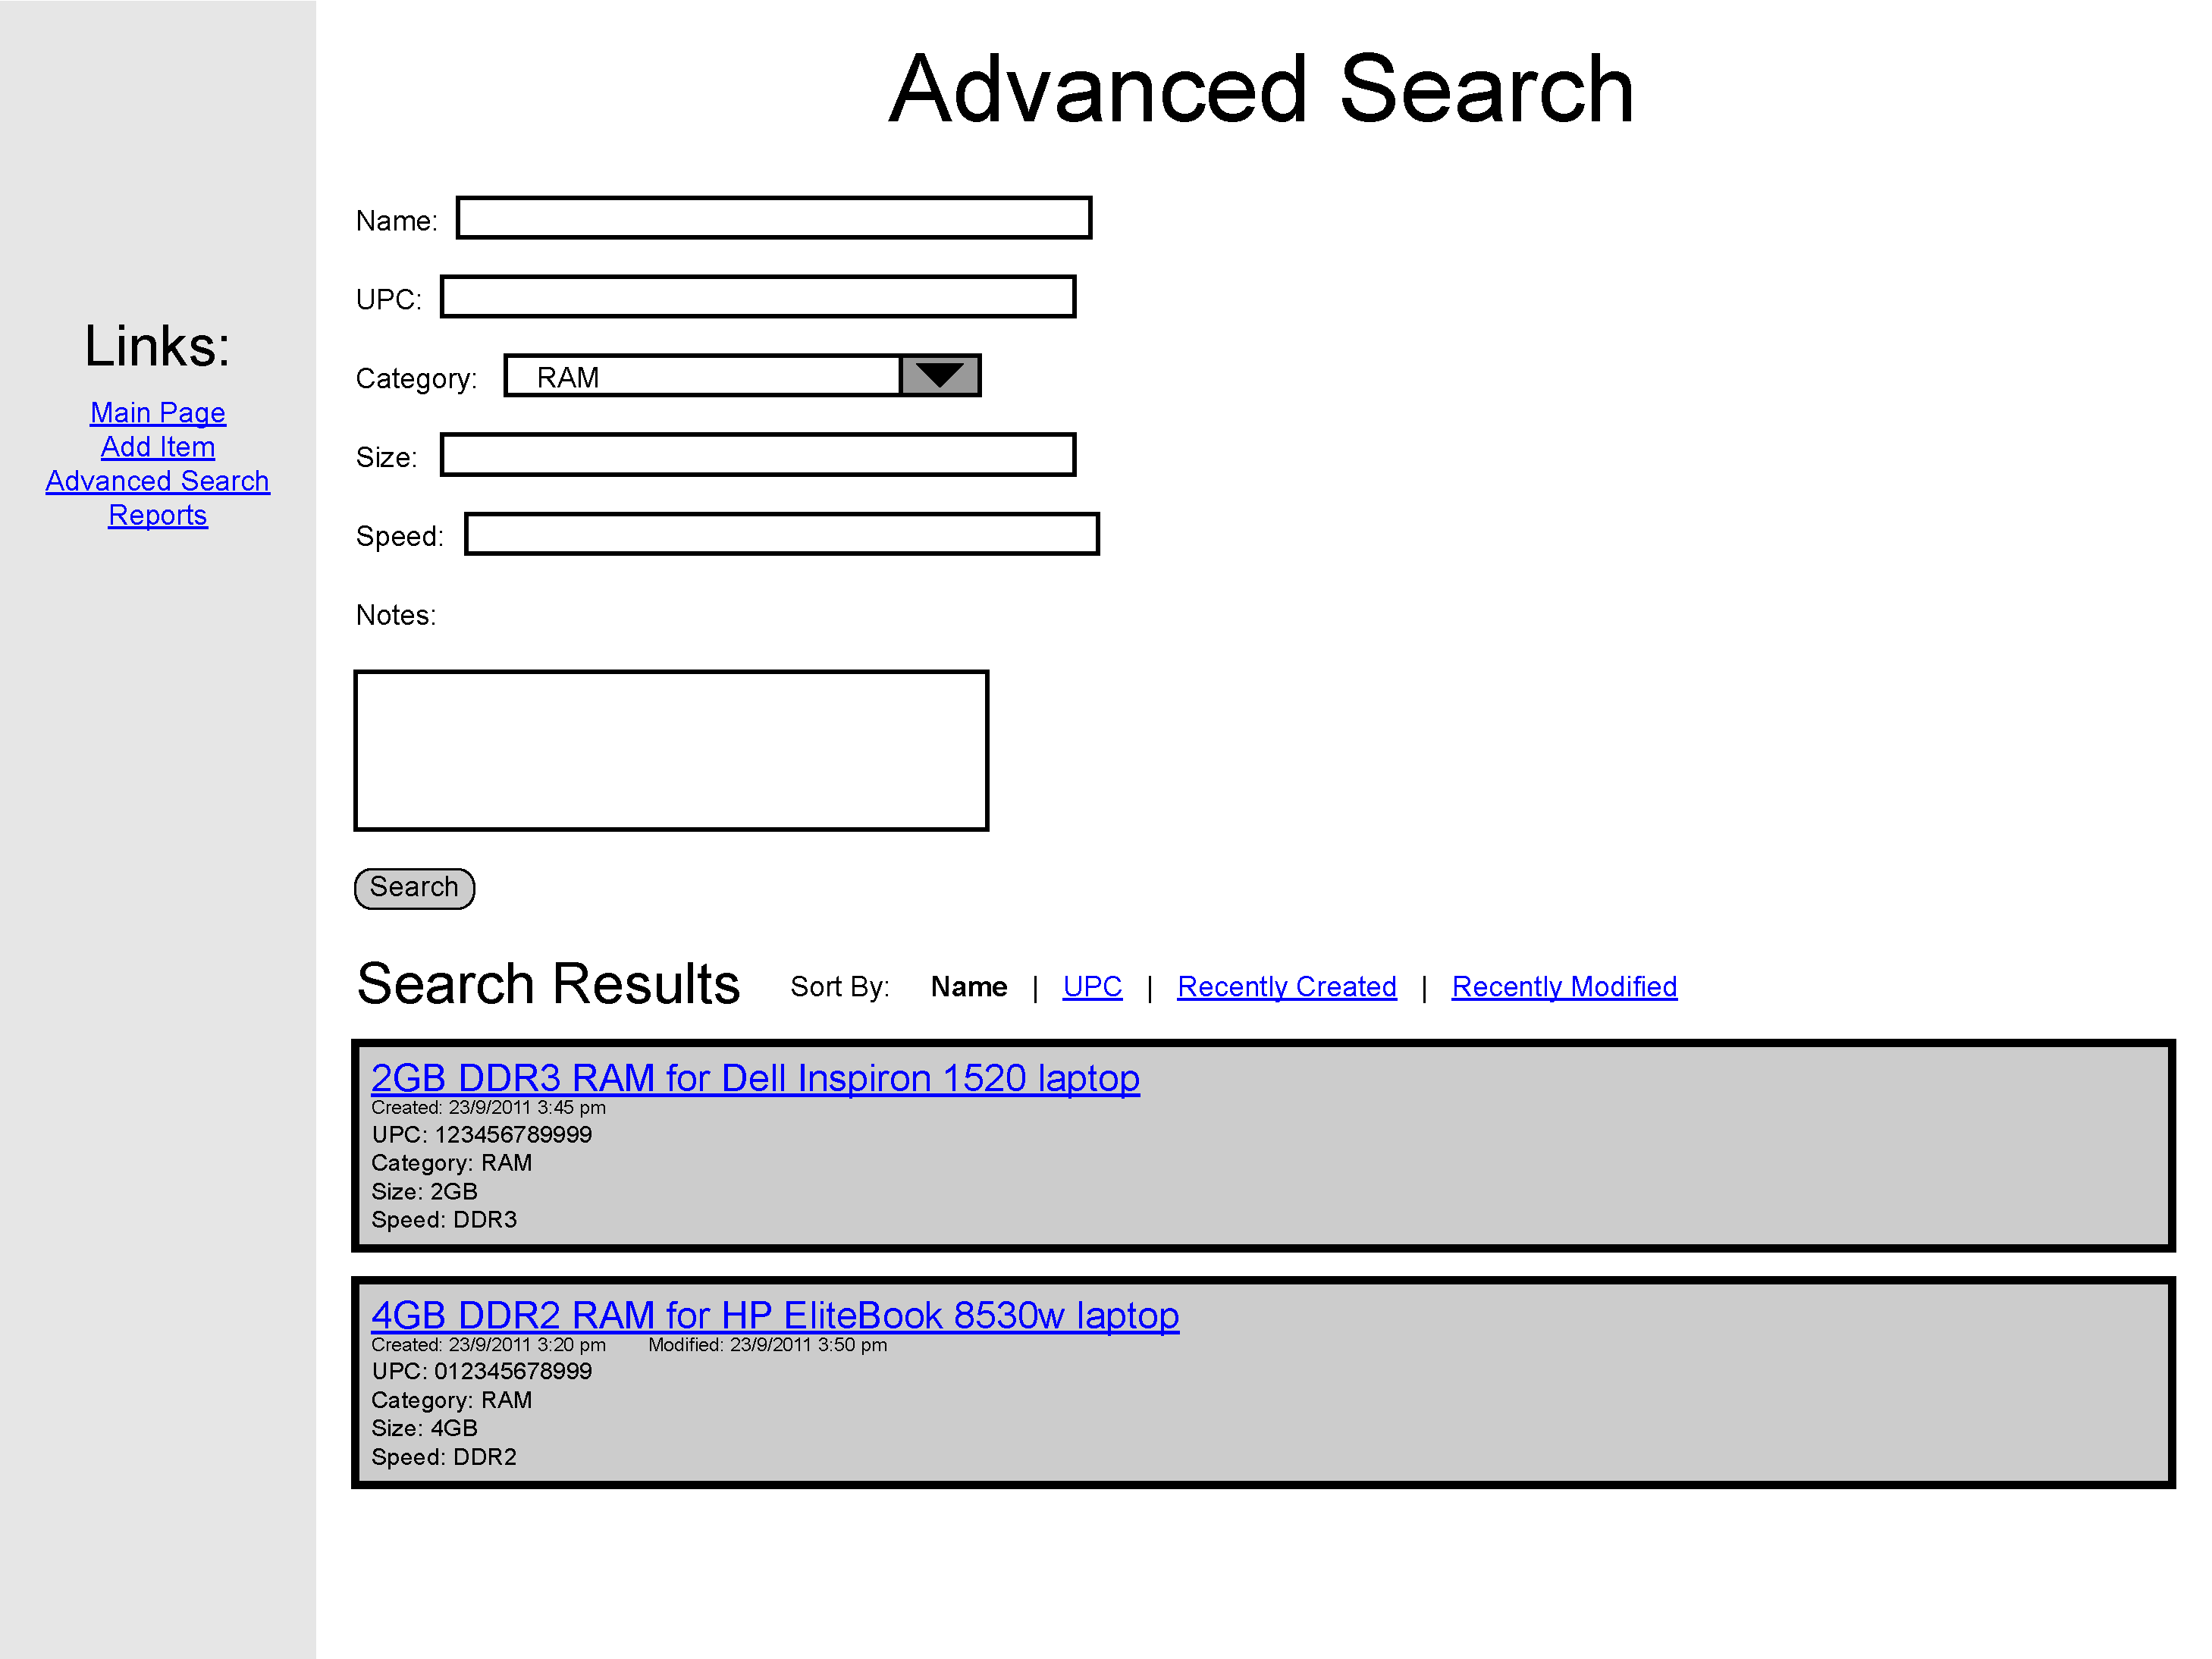
\includegraphics[keepaspectratio, width=4.5in]{sortResultsF0S0.pdf} \\
The advanced search page with results sorted by the default of Name
\end{tabular}\\
~\\
~\\
\begin{tabular}{ p{4.5in} }
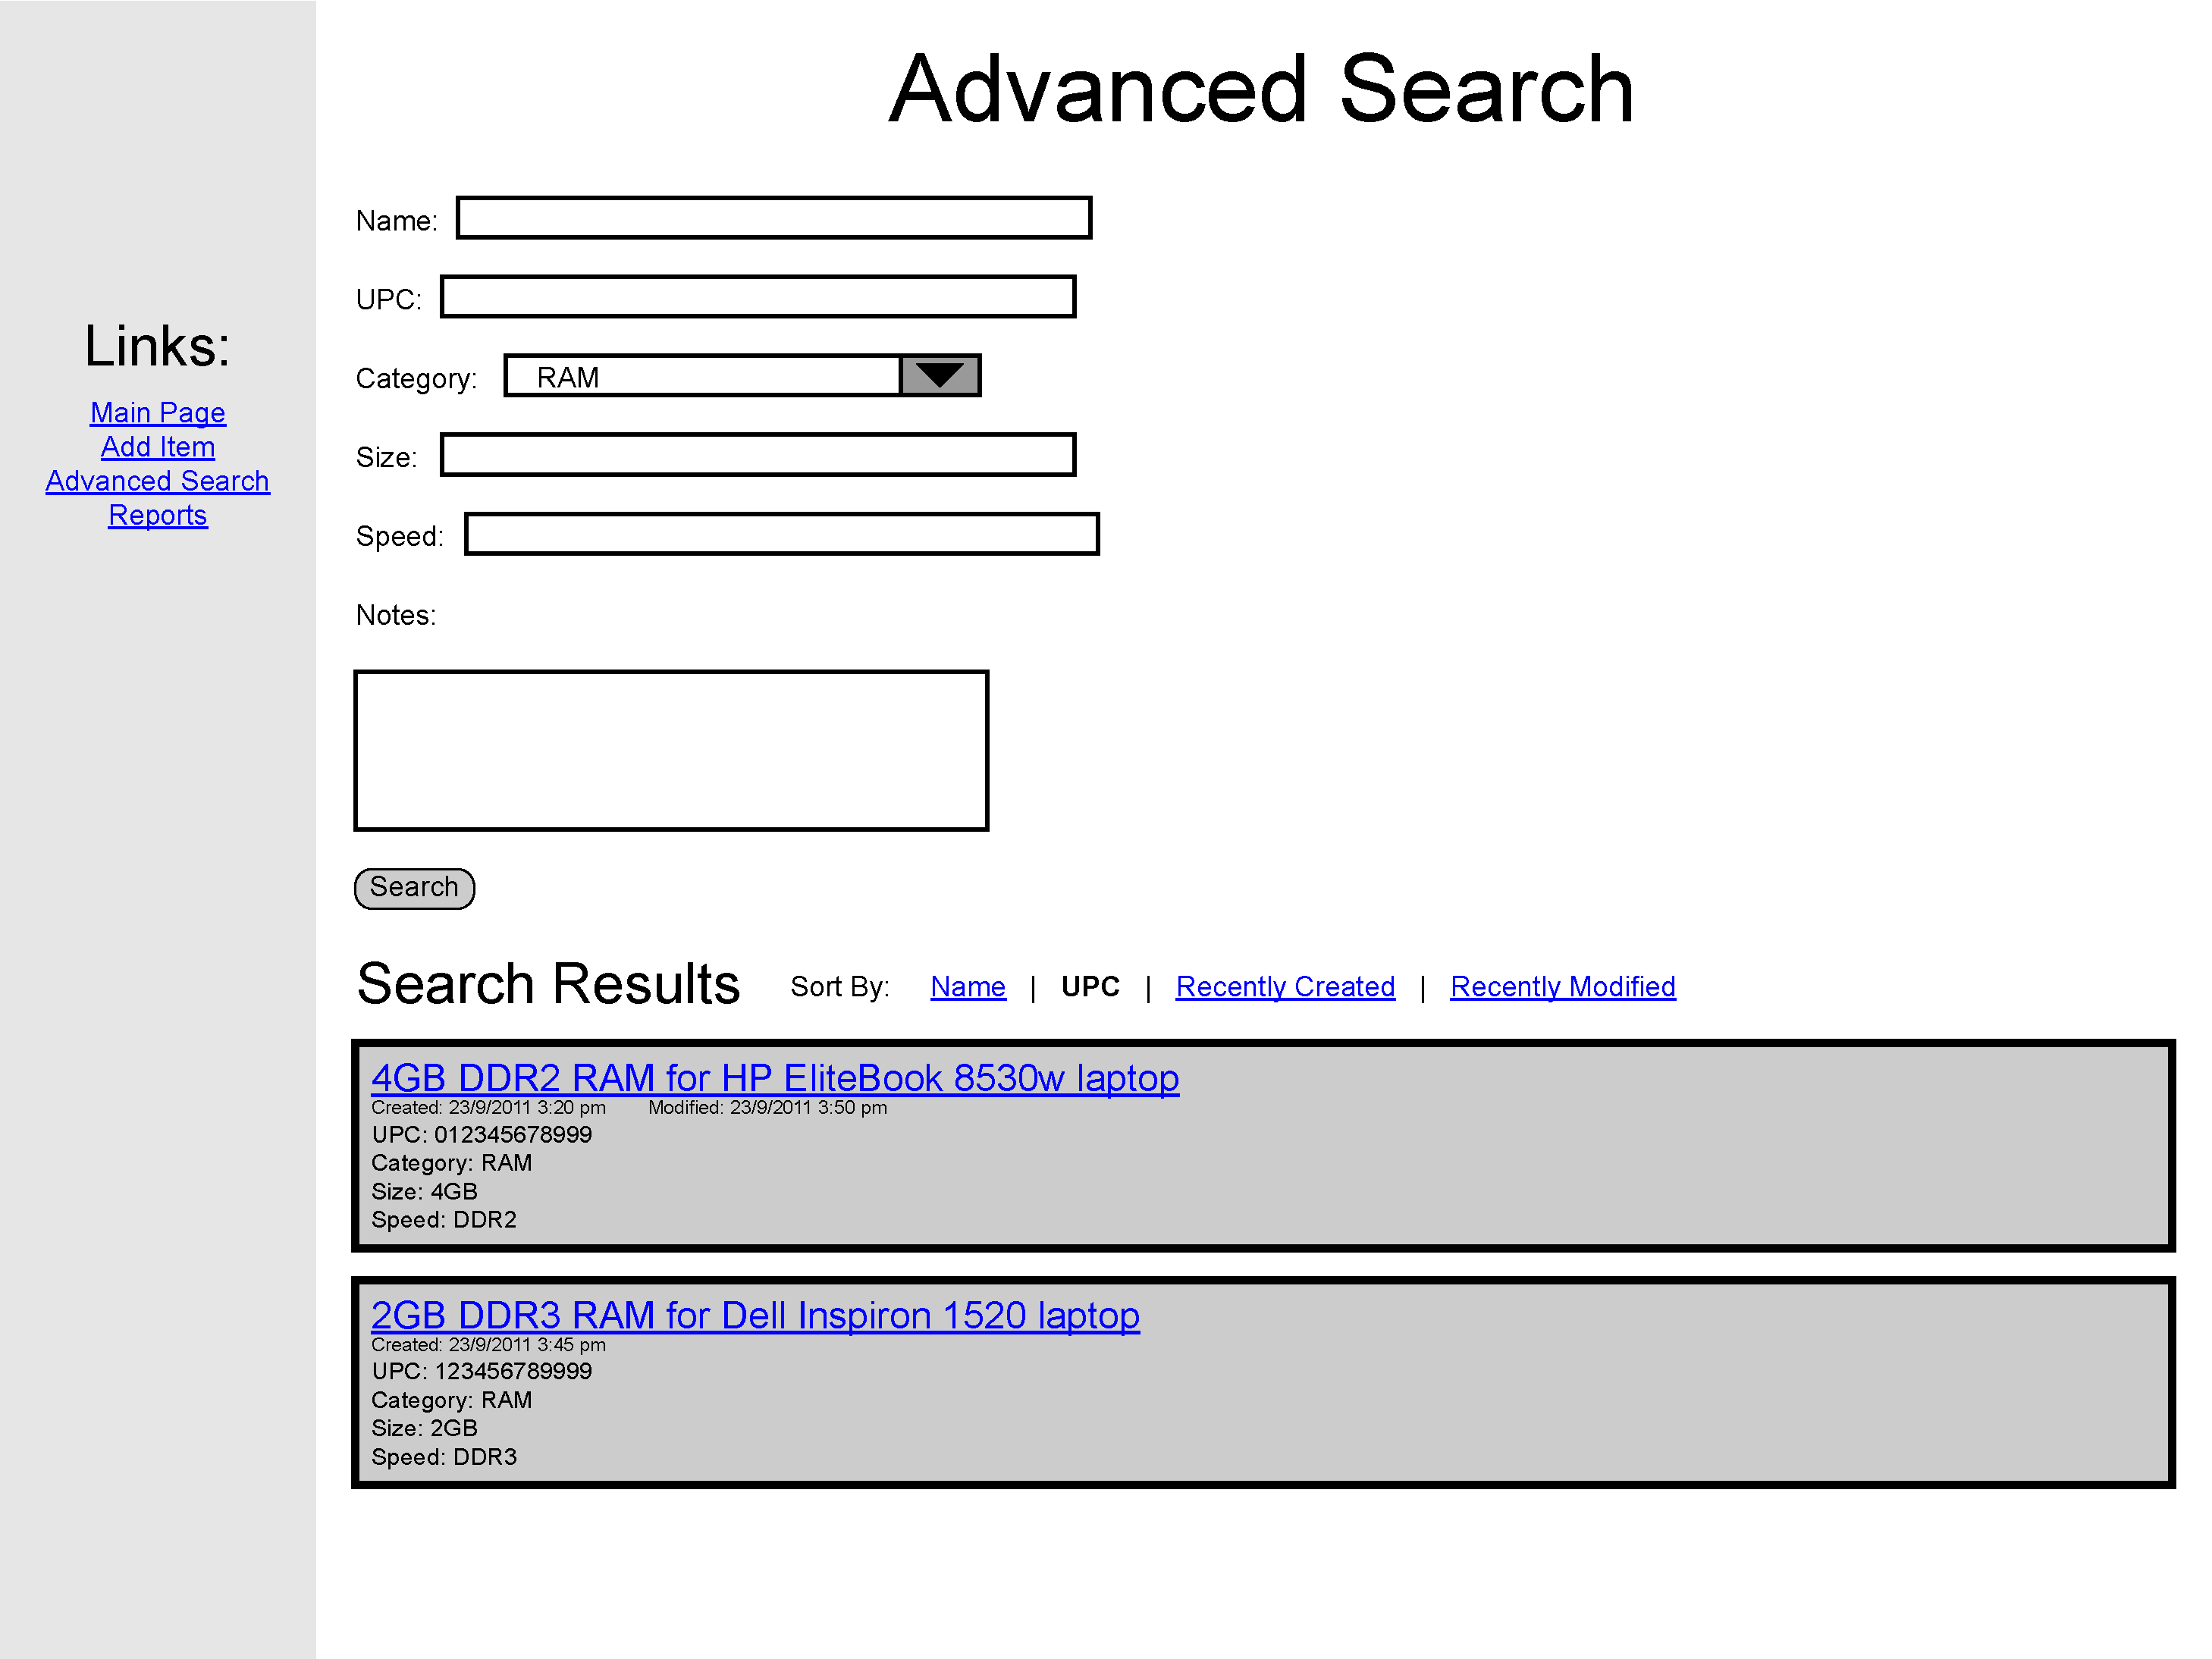
\includegraphics[keepaspectratio, width=4.5in]{sortResultsF0S1.pdf} \\
The advanced search page with results sorted by the user's choice of UPC
\end{tabular}\\
~\\
~\\
\begin{tabular}{ p{4.5in} }
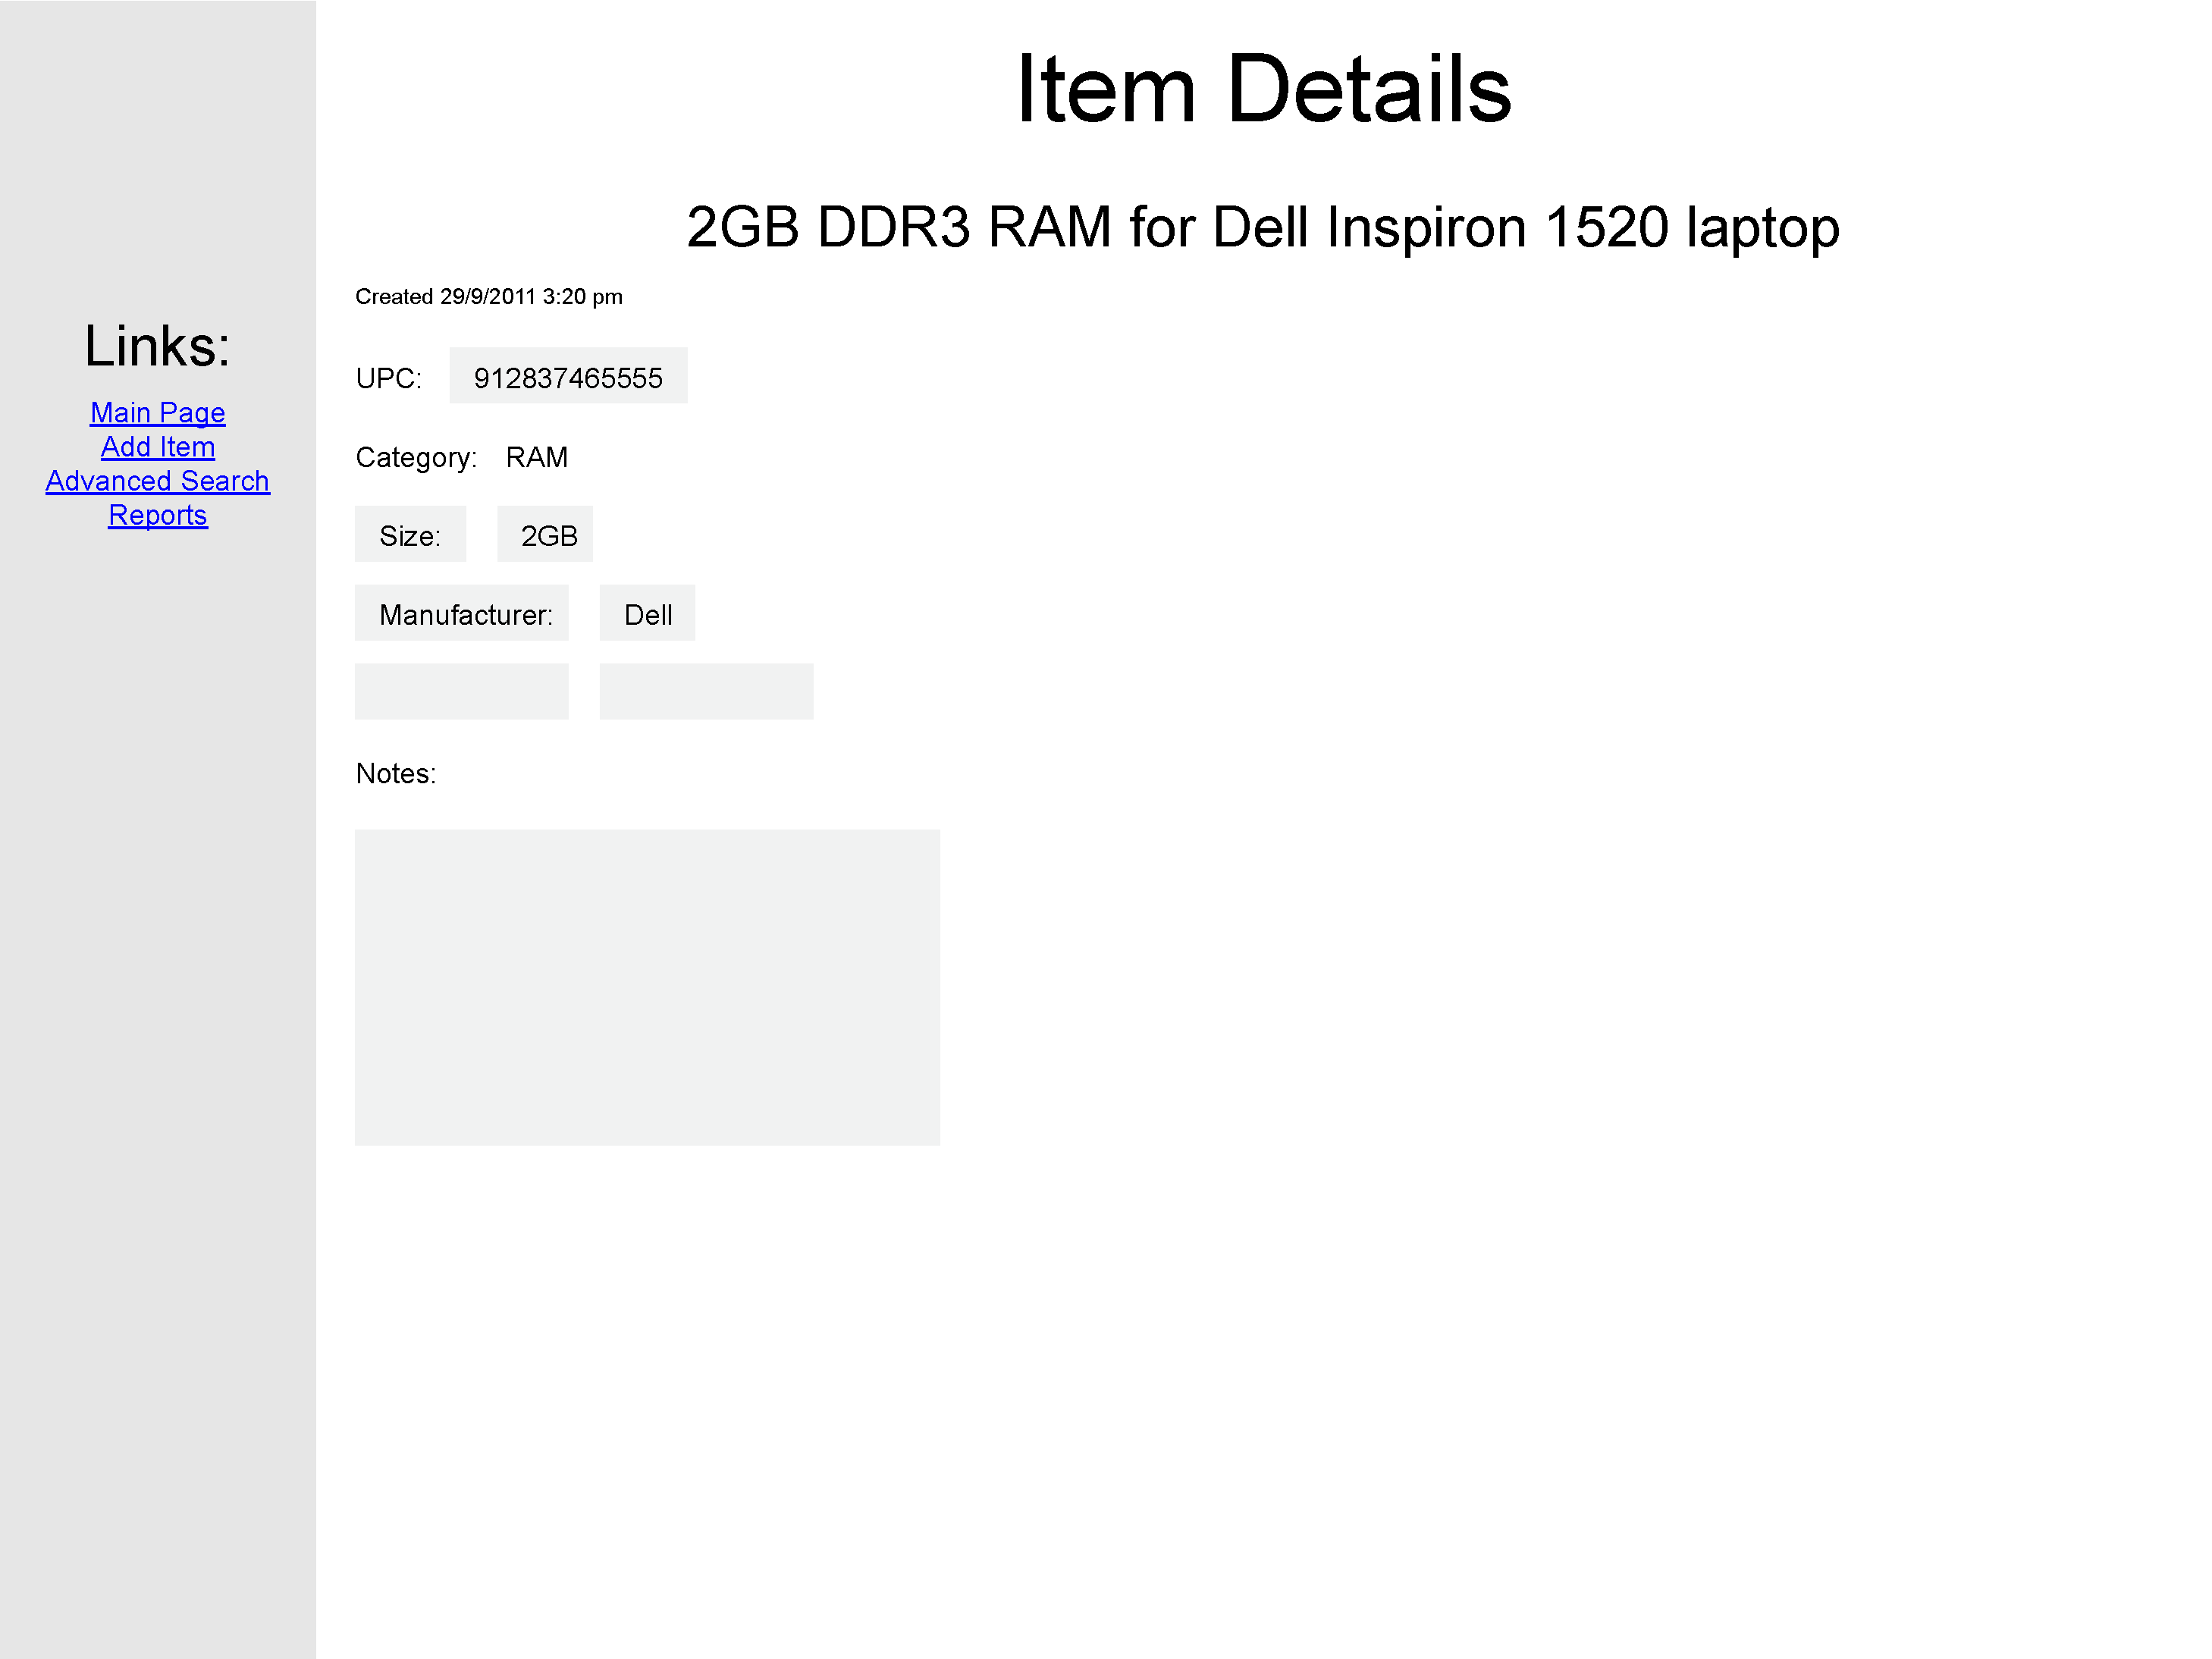
\includegraphics[keepaspectratio, width=4.5in]{viewDetailsF0S1.pdf} \\
The item details page in its initial state
\end{tabular}\\
~\\
~\\
\begin{tabular}{ p{4.5in} }
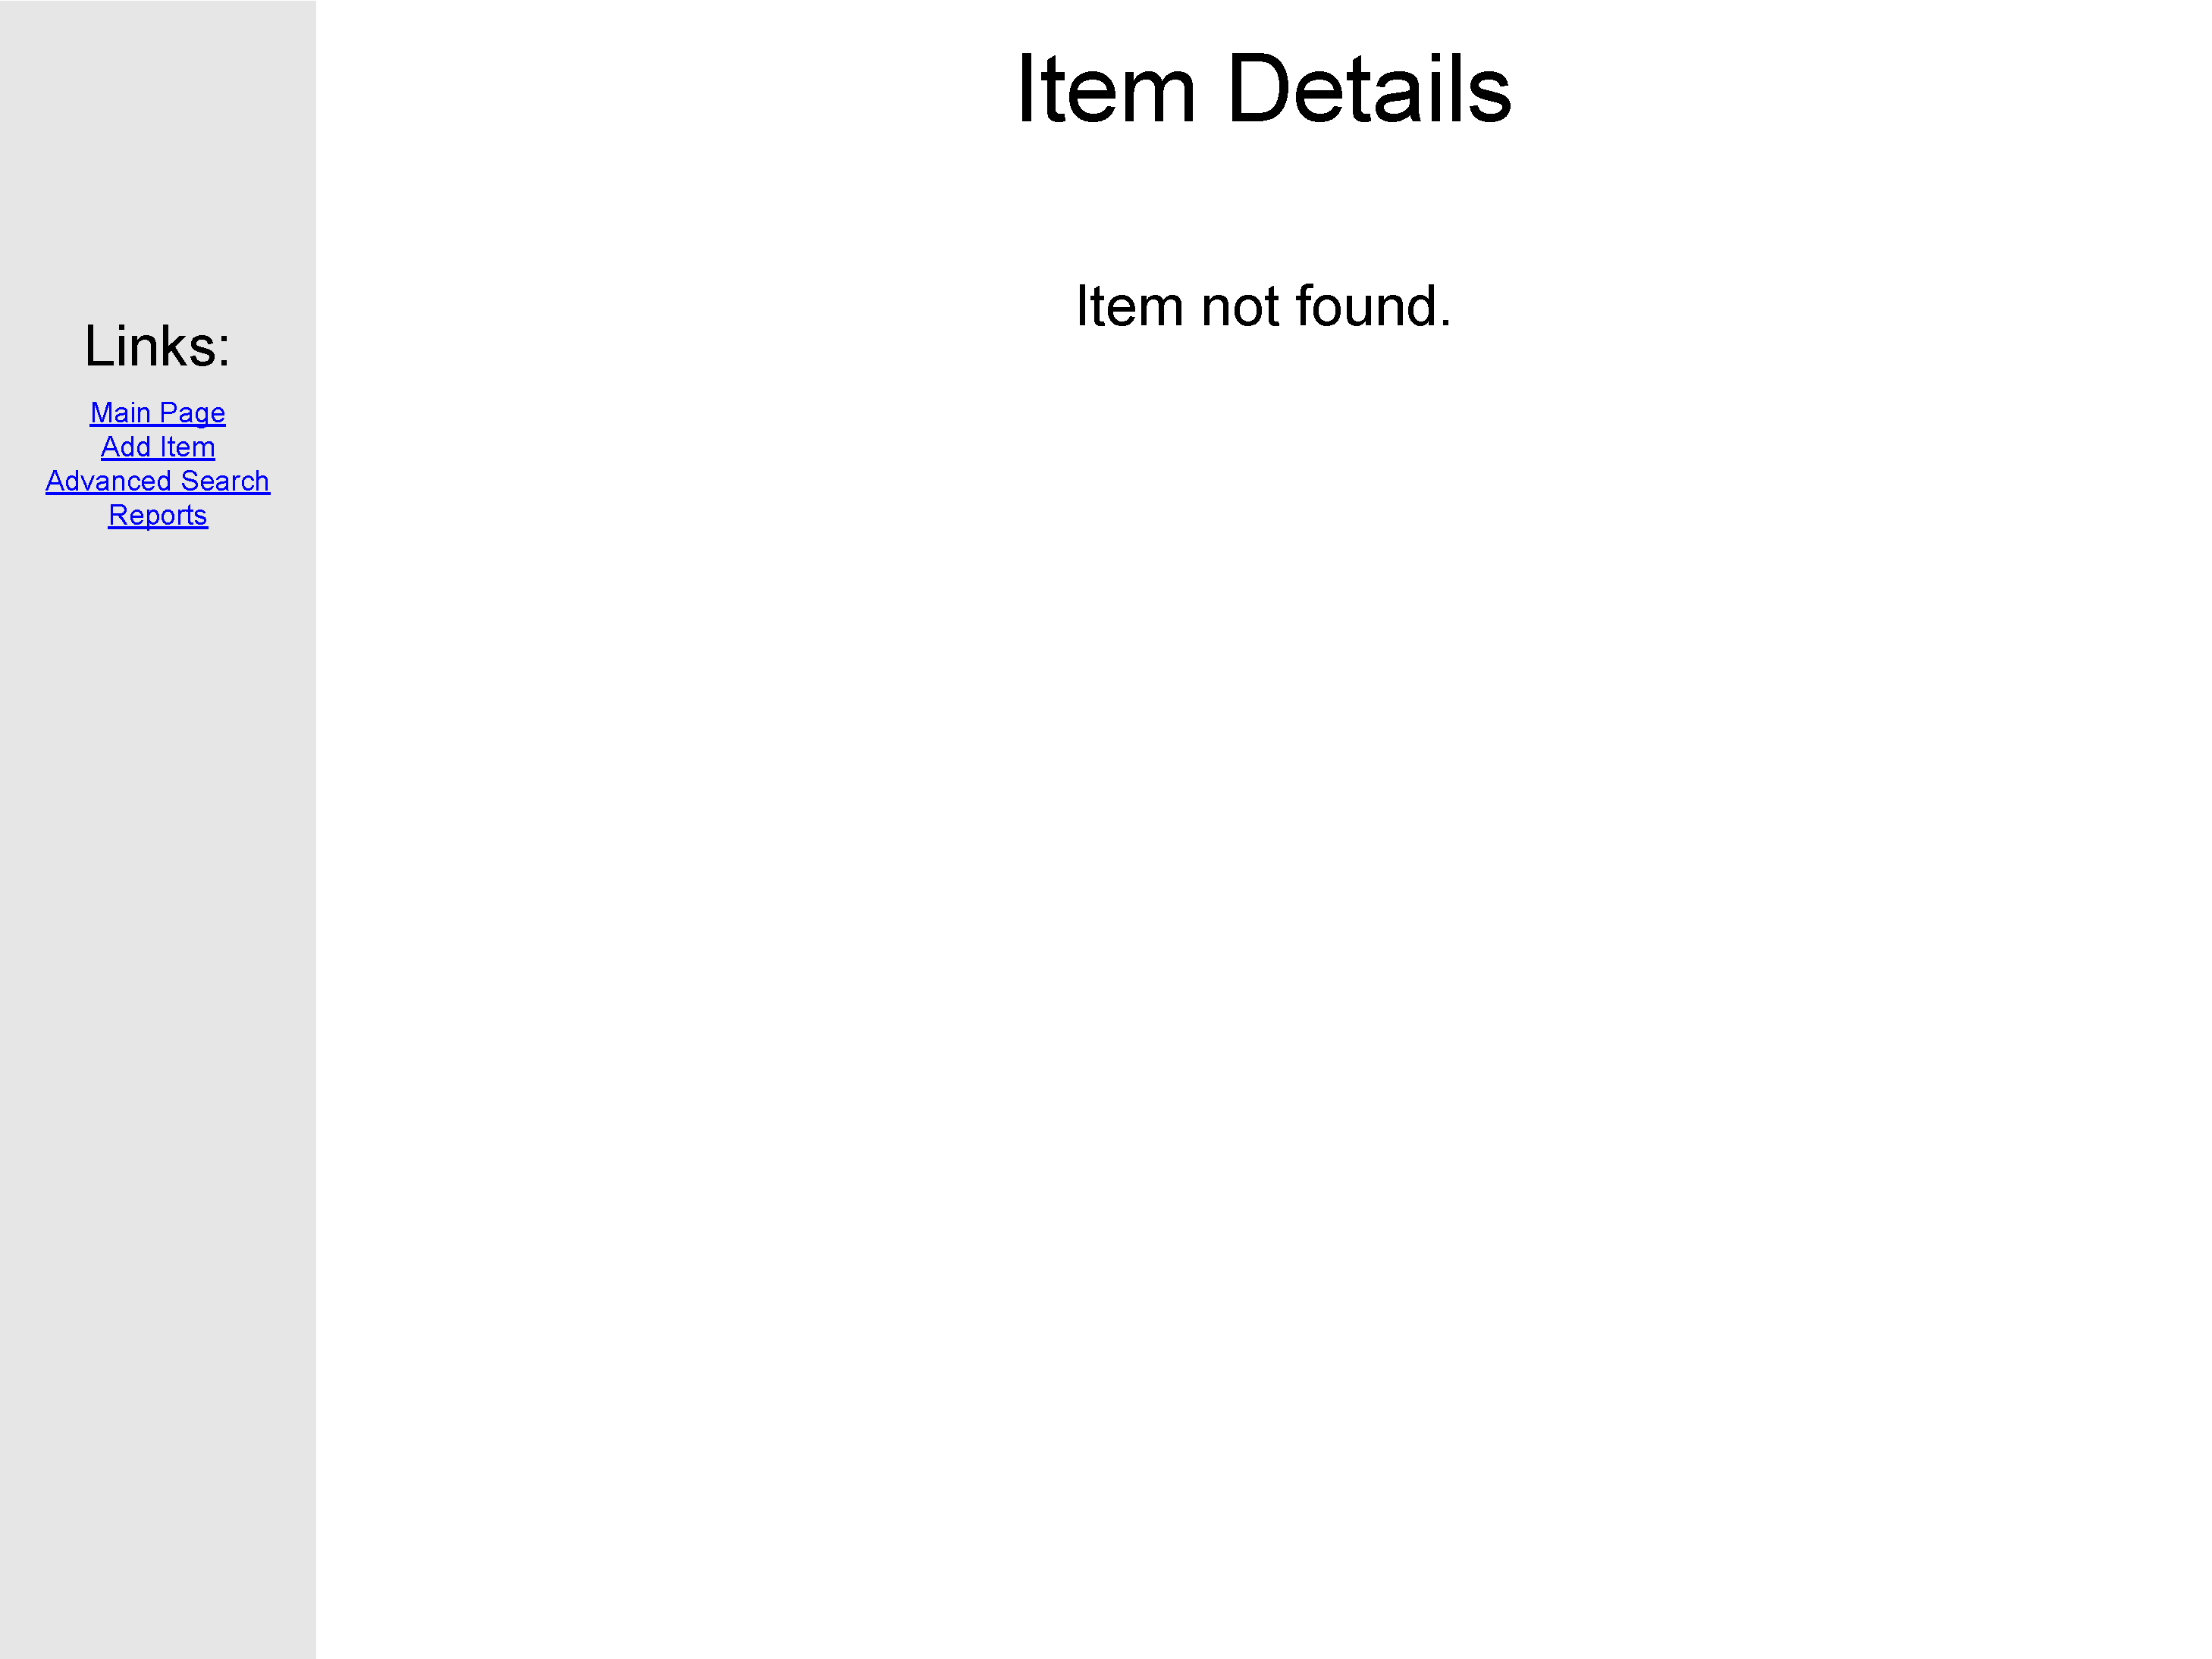
\includegraphics[keepaspectratio, width=4.5in]{viewDetailsF1S1.pdf} \\
The item details page for an item that could not be found.
\end{tabular}\\
~\\
~\\
\begin{tabular}{ p{4.5in} }
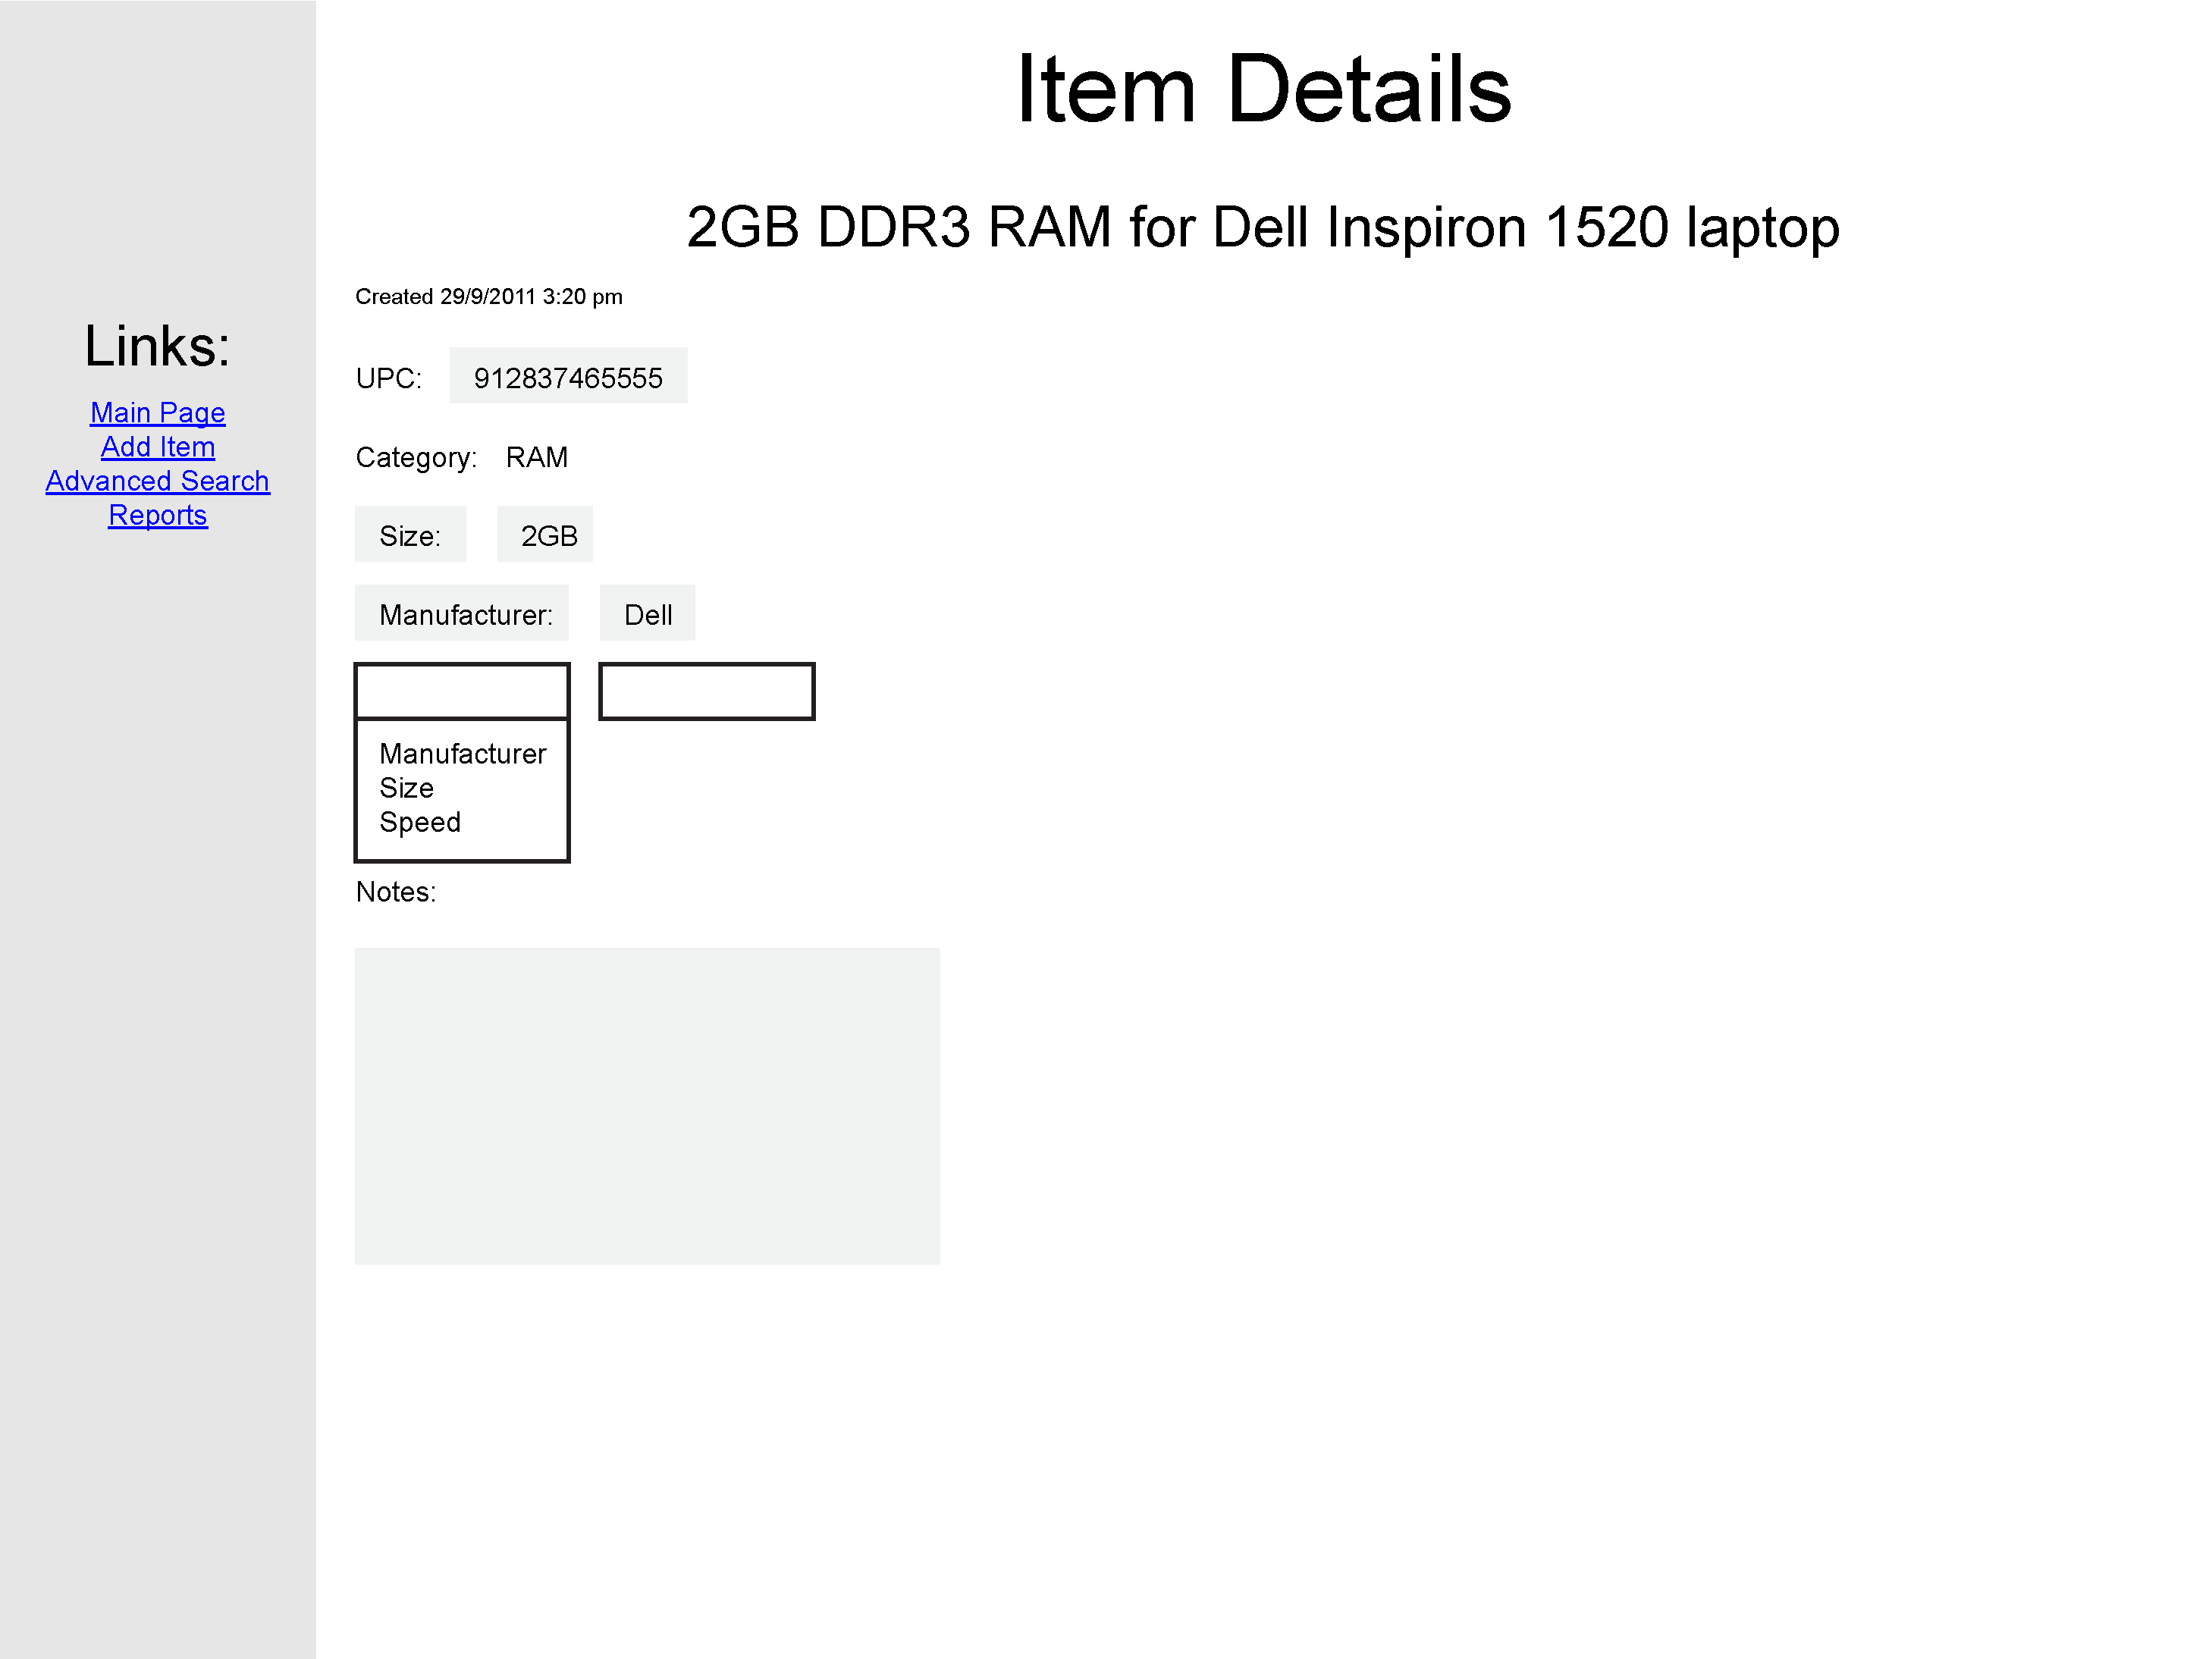
\includegraphics[keepaspectratio, width=4.5in]{modifyDetailsF0S1.pdf} \\
The item details page after the user has clicked on the empty attribute key field and caused the element to be replaced with a autocomplete text field
\end{tabular}\\
~\\
~\\
\begin{tabular}{ p{4.5in} }
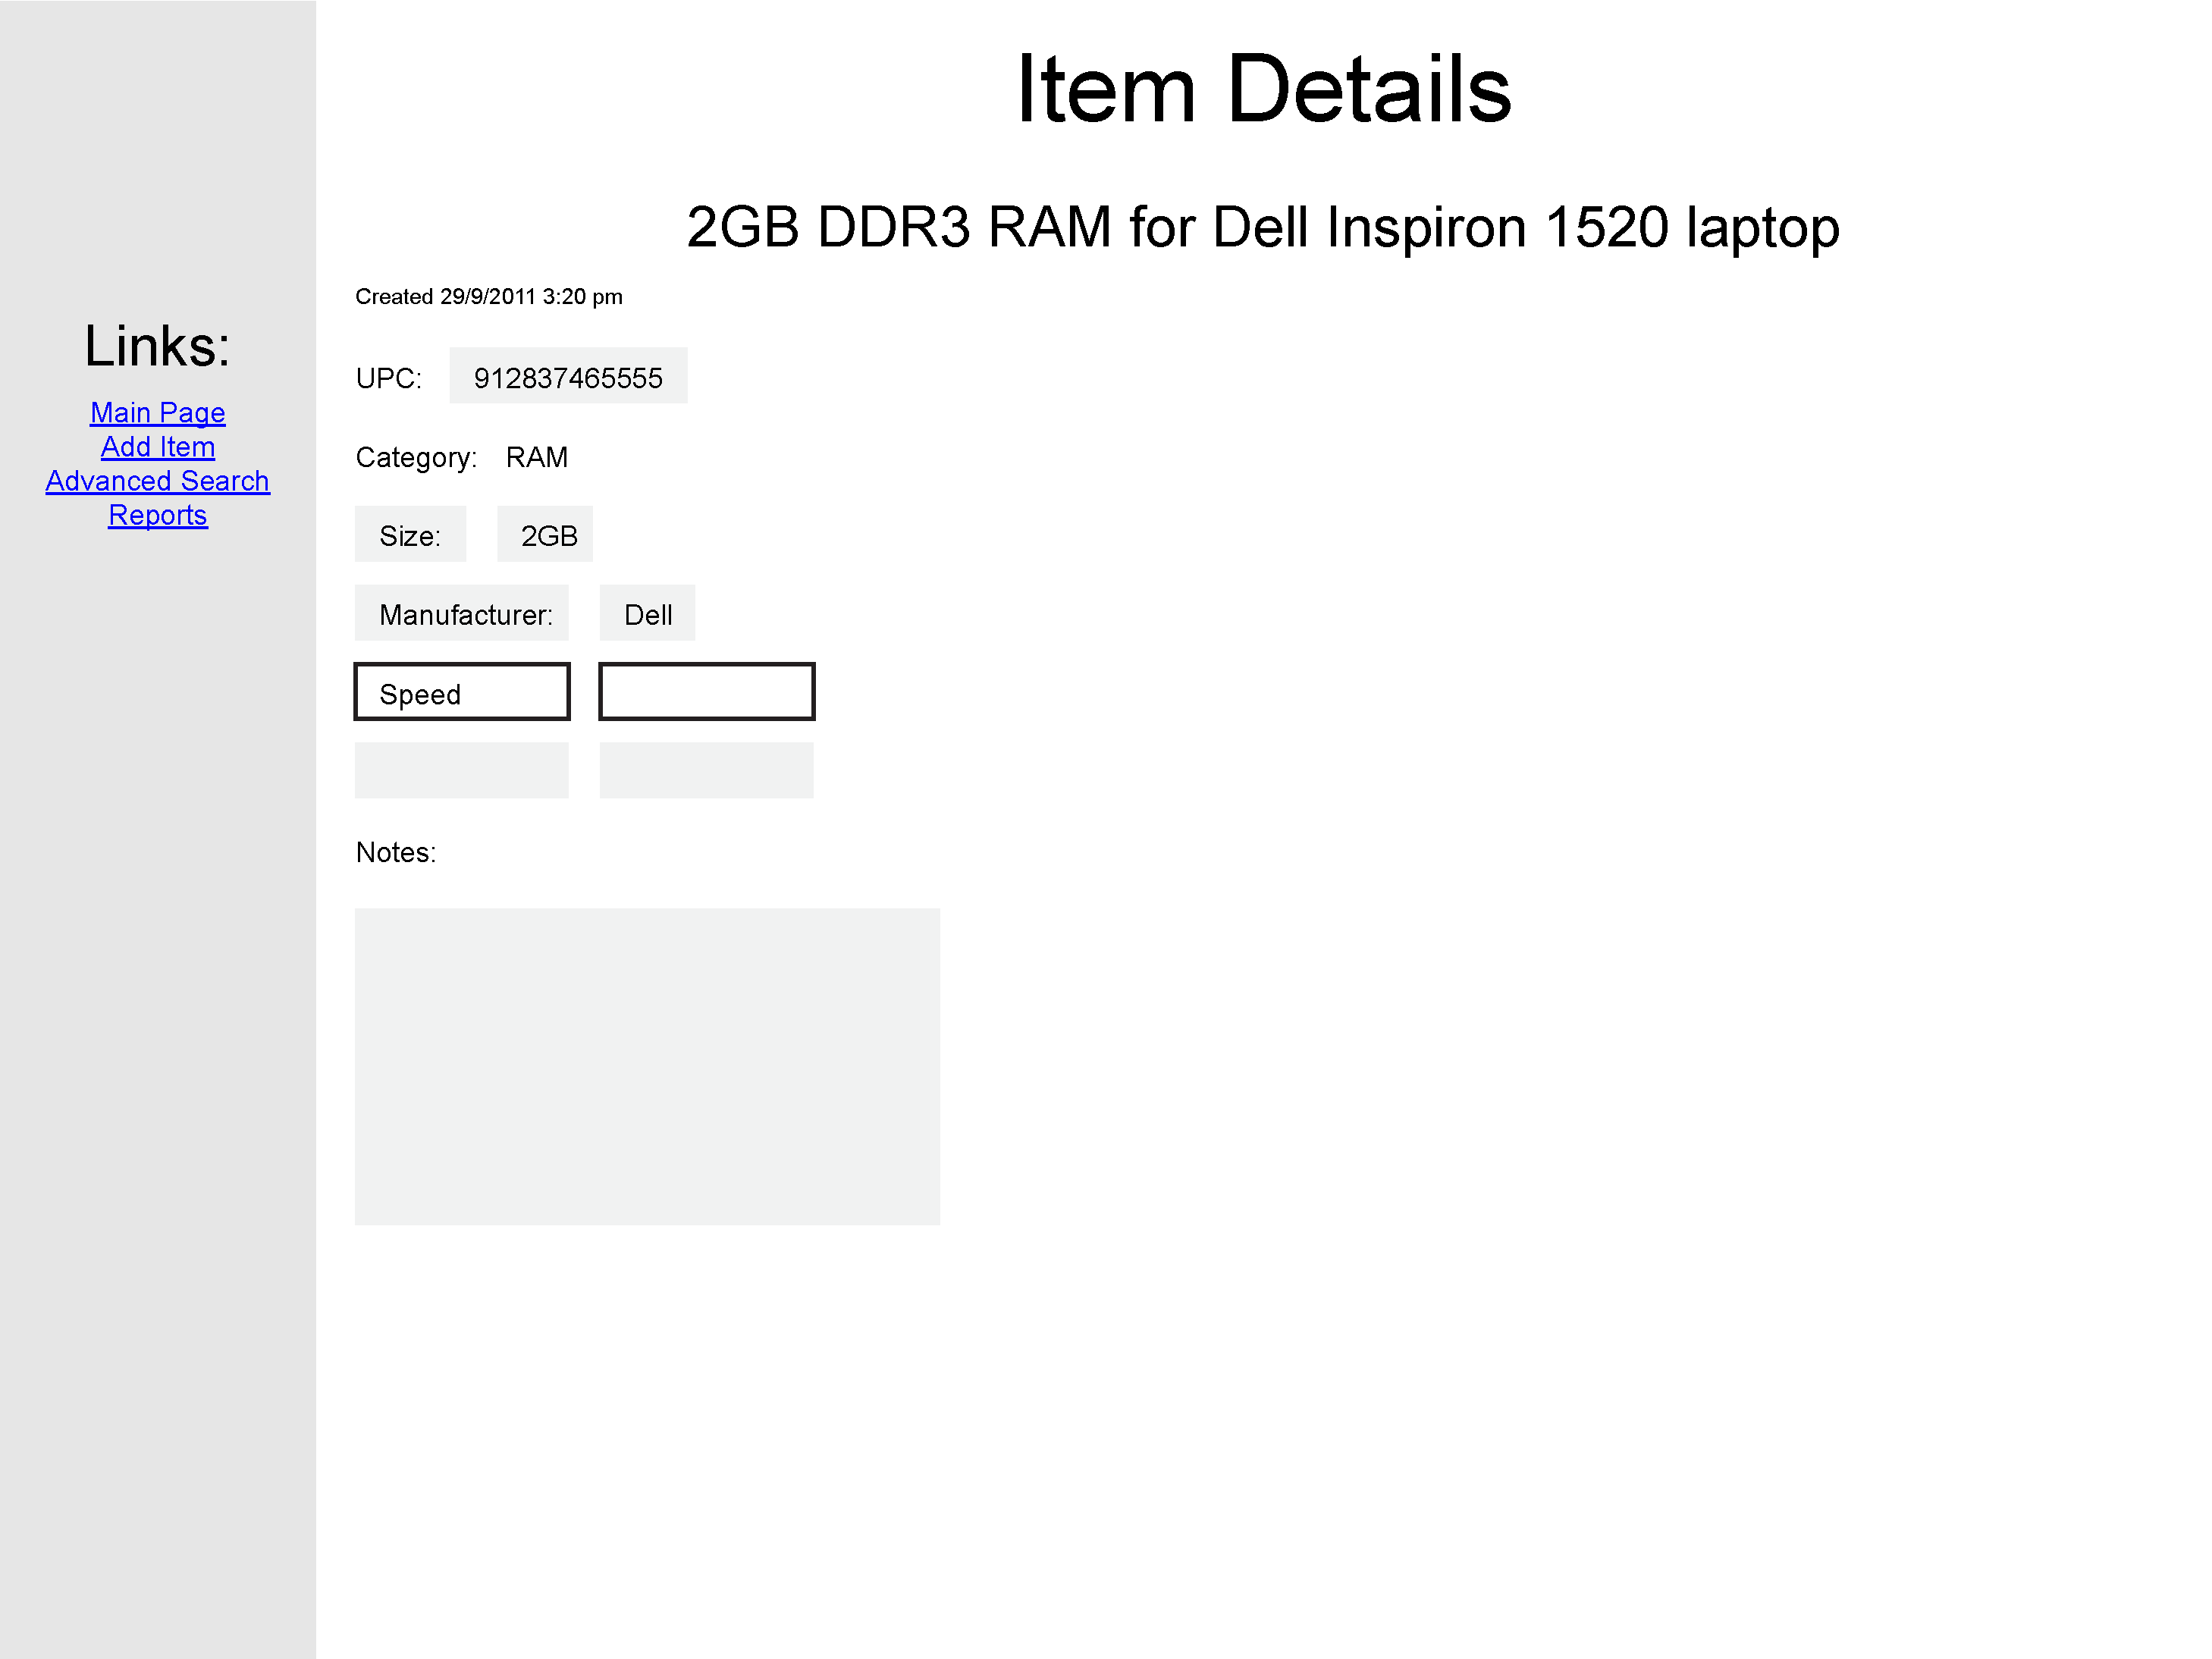
\includegraphics[keepaspectratio, width=4.5in]{modifyDetailsF0S2.pdf} \\
The item details page after a attribute key has been selected
\end{tabular}\\
~\\
~\\
\begin{tabular}{ p{4.5in} }
\includegraphics[keepaspectratio, width=4.5in]{modifyDetailsF0S3.pdf} \\
The item details page after the attribute key and value have been entered
\end{tabular}\\
~\\
~\\
\begin{tabular}{ p{4.5in} }
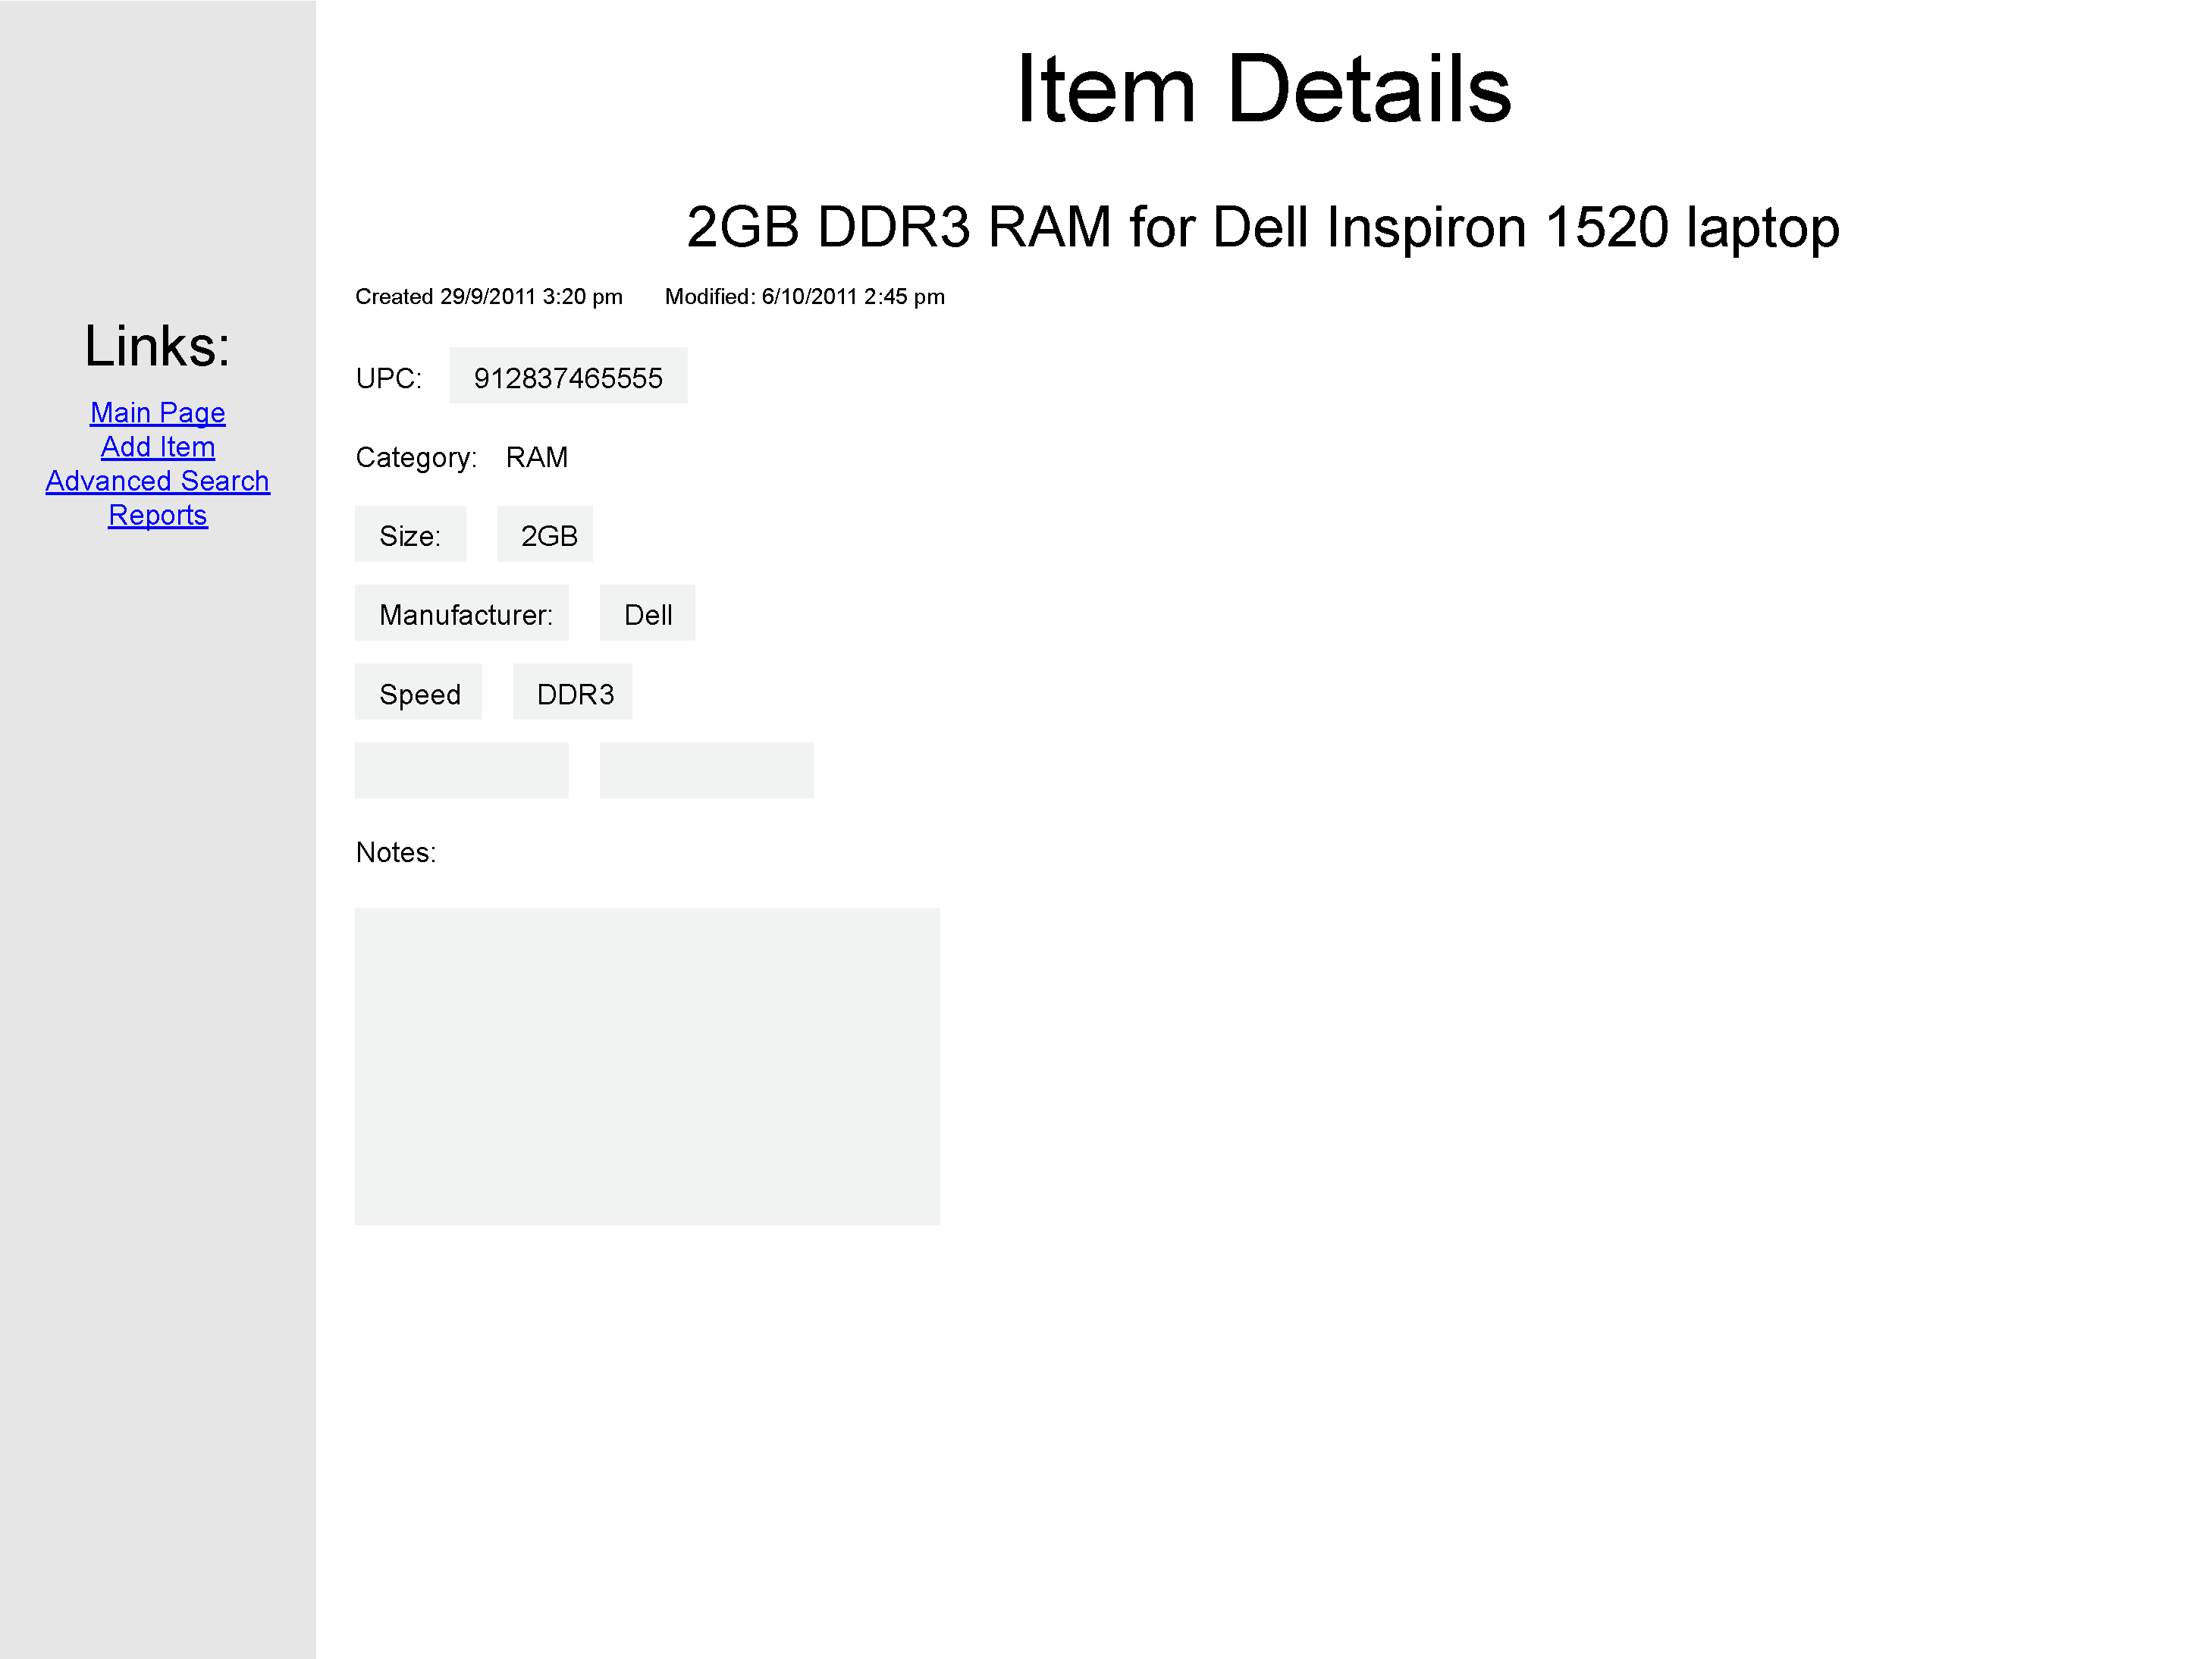
\includegraphics[keepaspectratio, width=4.5in]{modifyDetailsF0S4.pdf} \\
The item details page after the user has deselected the fields
\end{tabular}\\
~\\
~\\
\begin{tabular}{ p{4.5in} }
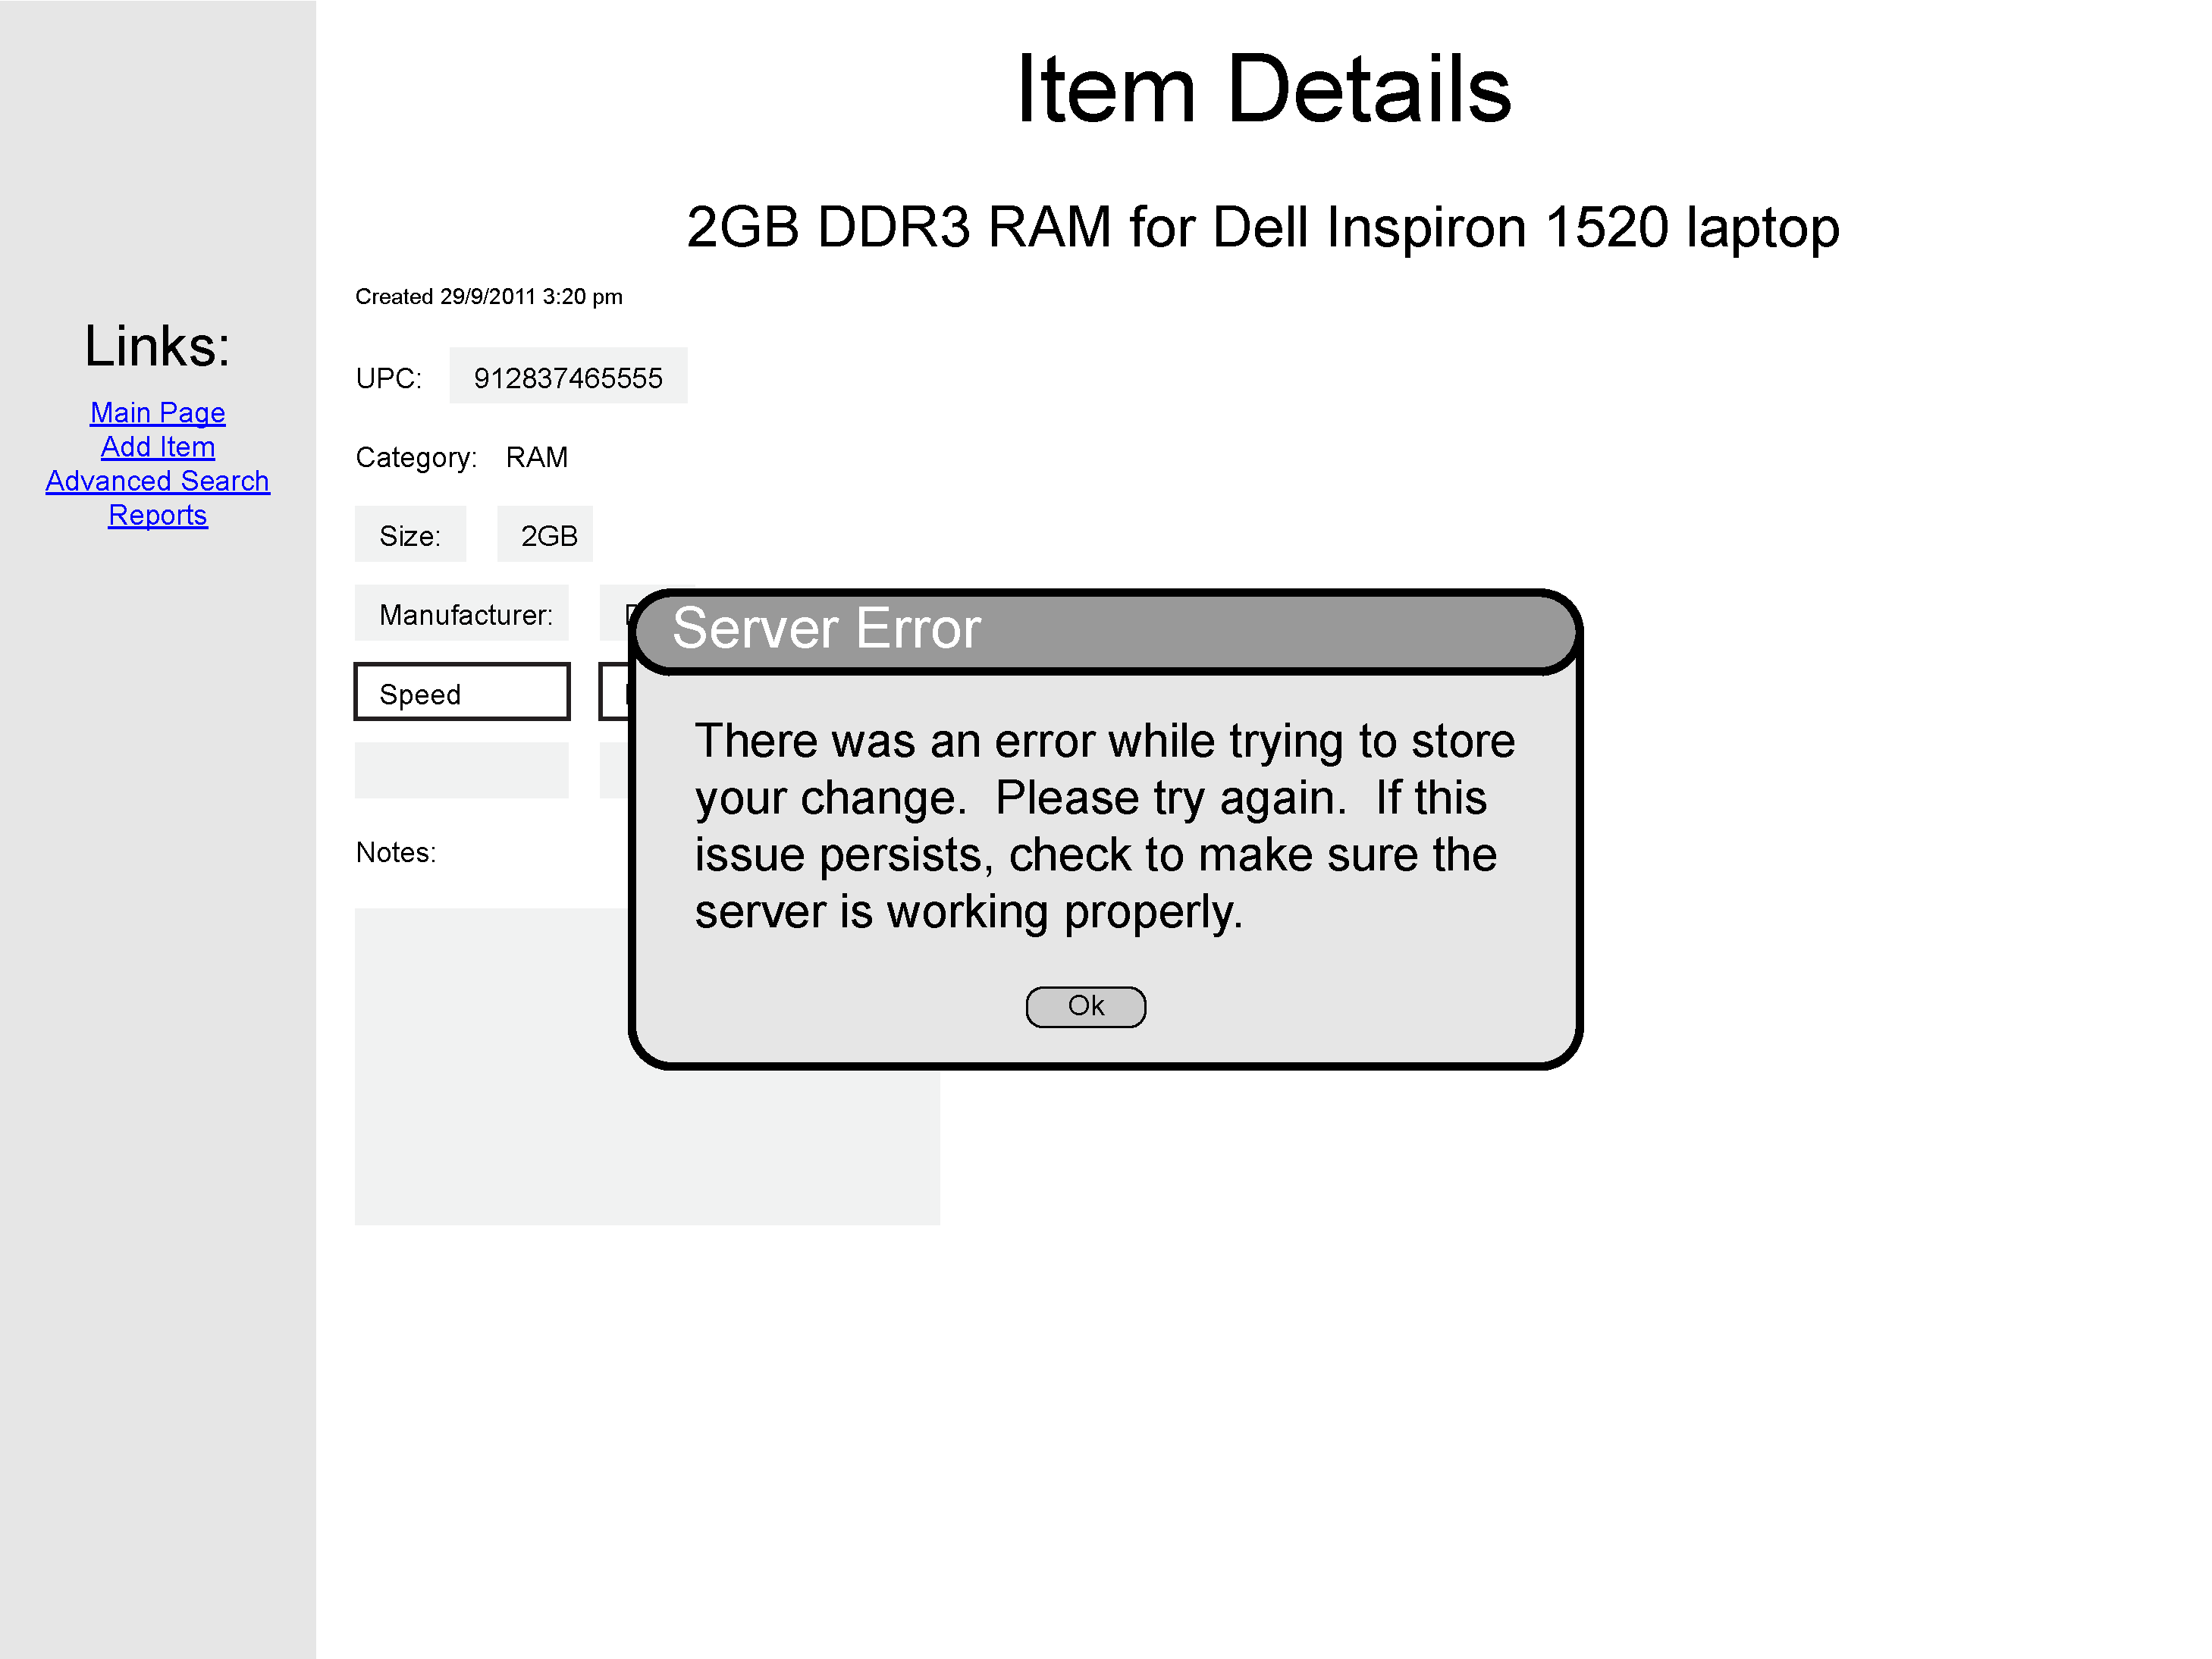
\includegraphics[keepaspectratio, width=4.5in]{modifyDetailsF1S4.pdf} \\
The item details page after the user has deselected the fields and the server has returned with an error
\end{tabular}\\
~\\
~\\
\begin{tabular}{ p{4.5in} }
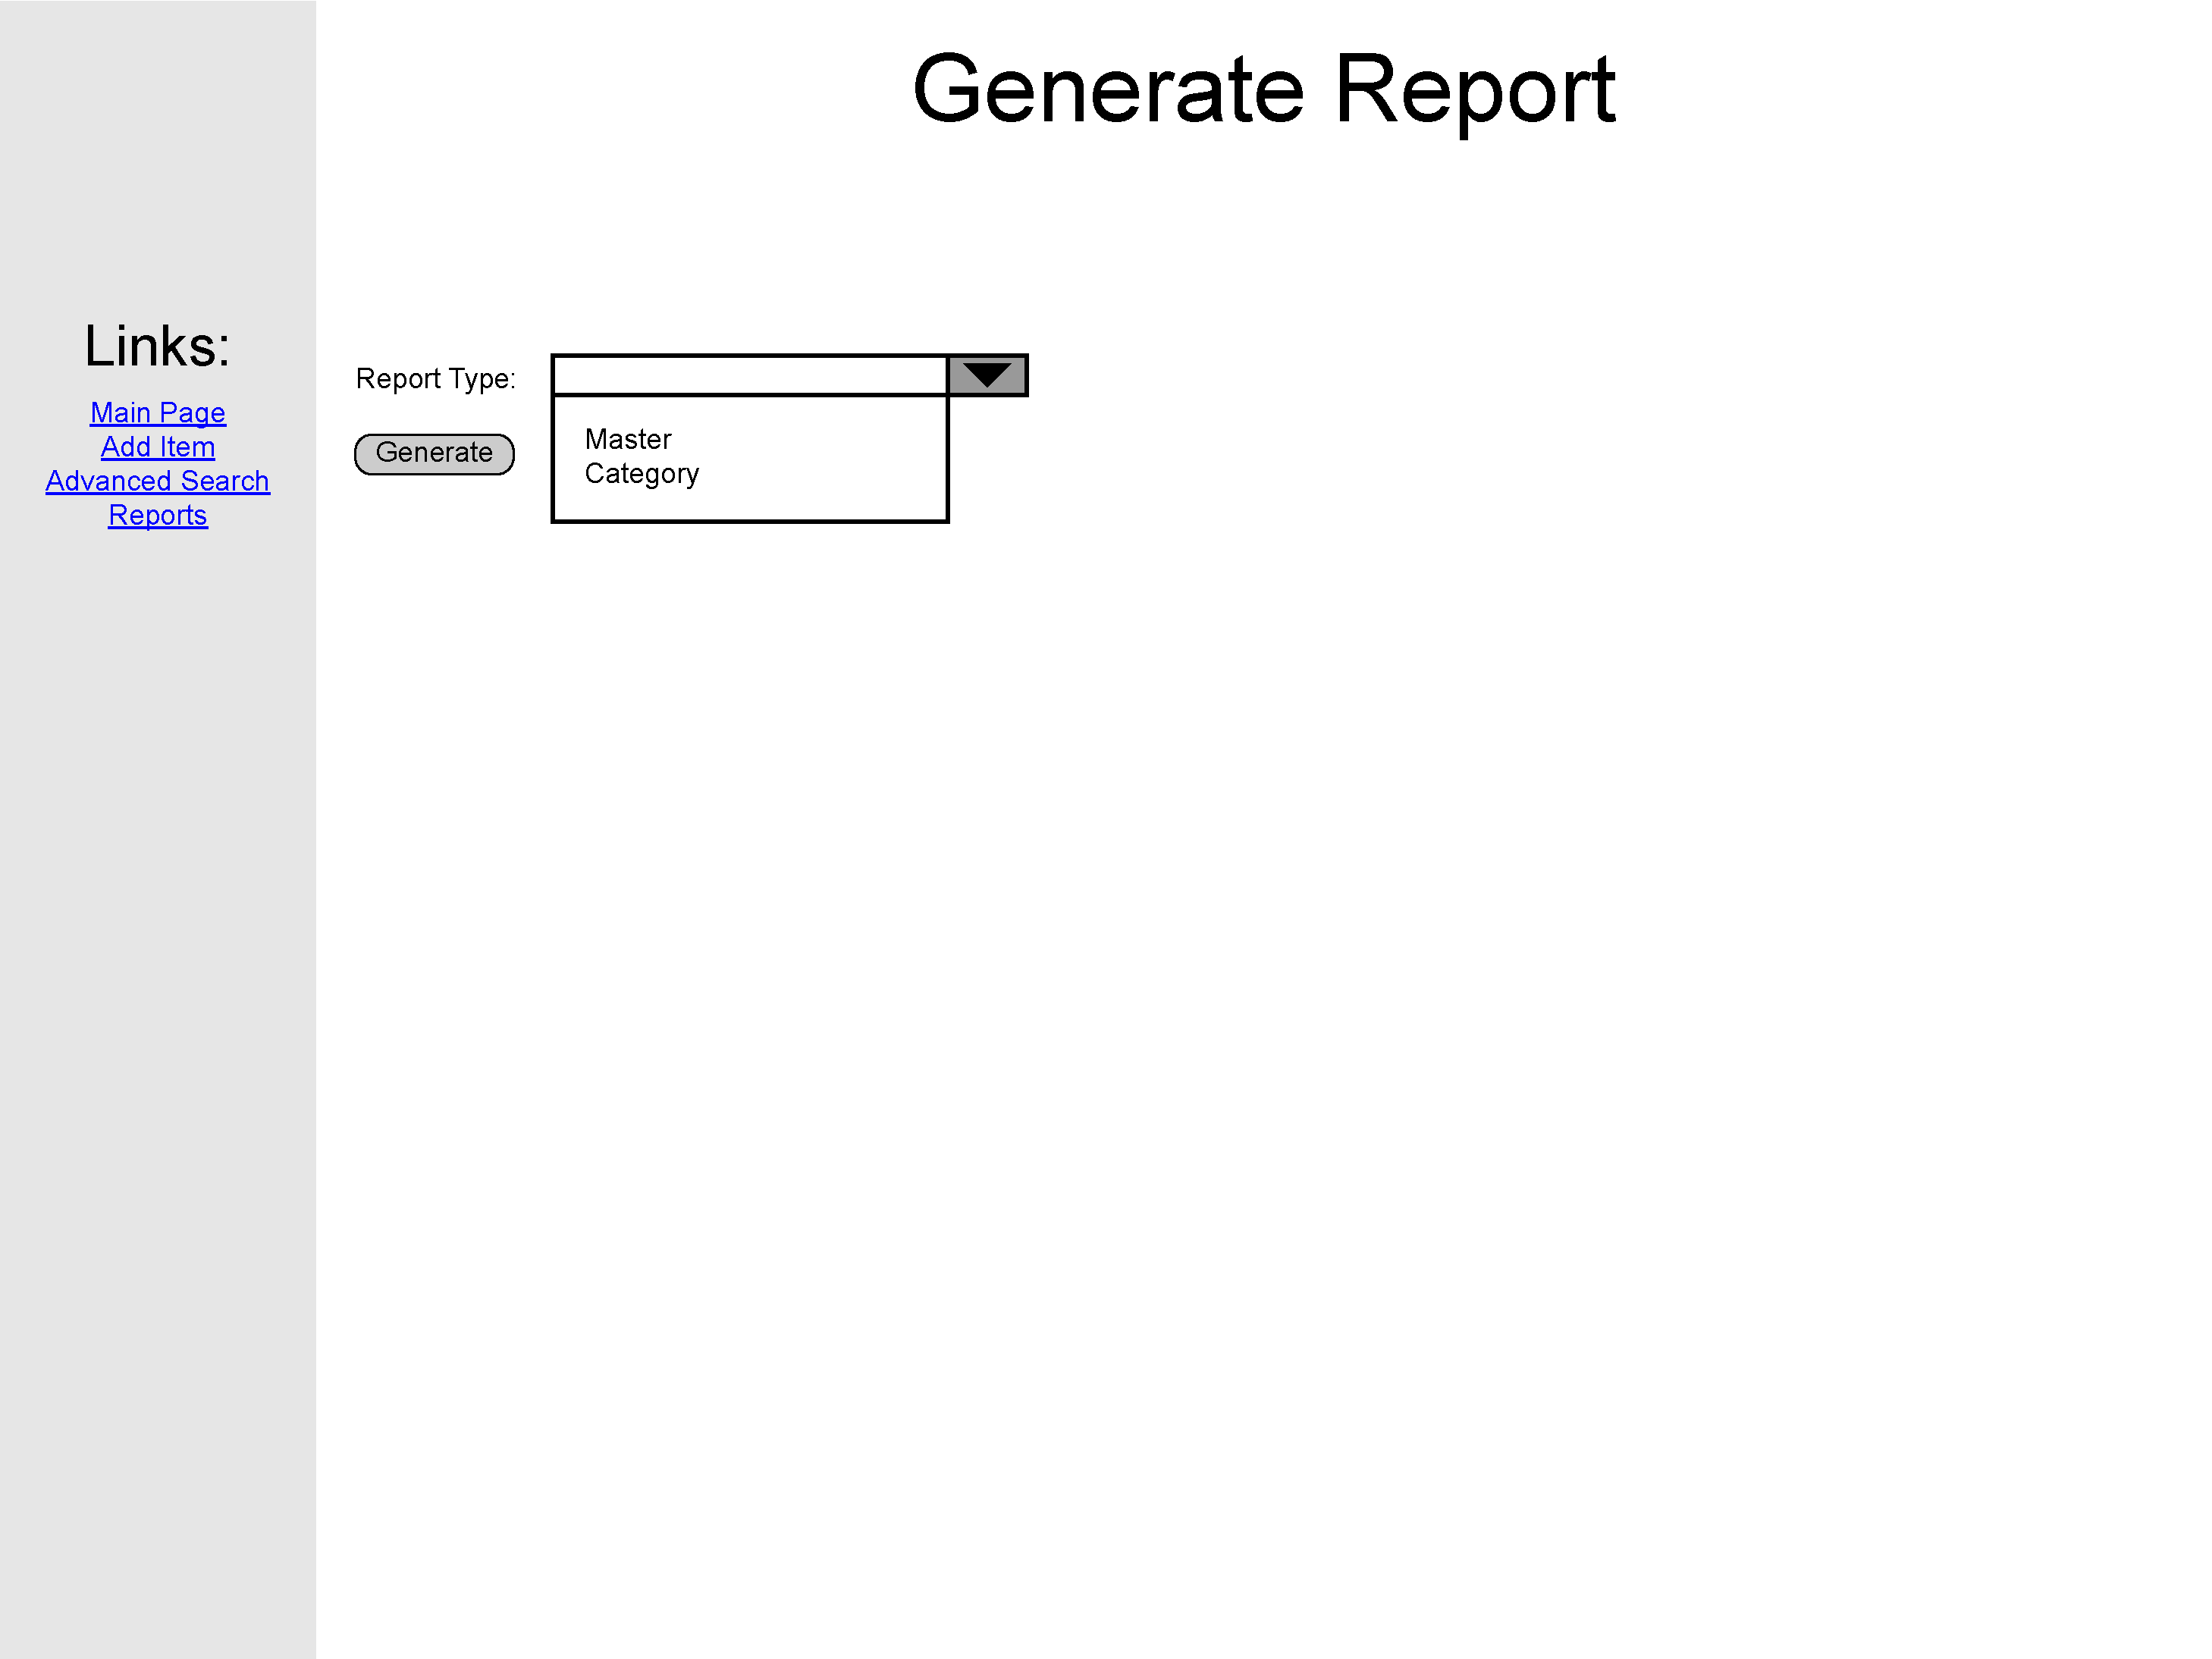
\includegraphics[keepaspectratio, width=4.5in]{generateReportF0S1.pdf} \\
The generate report page before a report type has been selected
\end{tabular}\\
~\\
~\\
\begin{tabular}{ p{4.5in} }
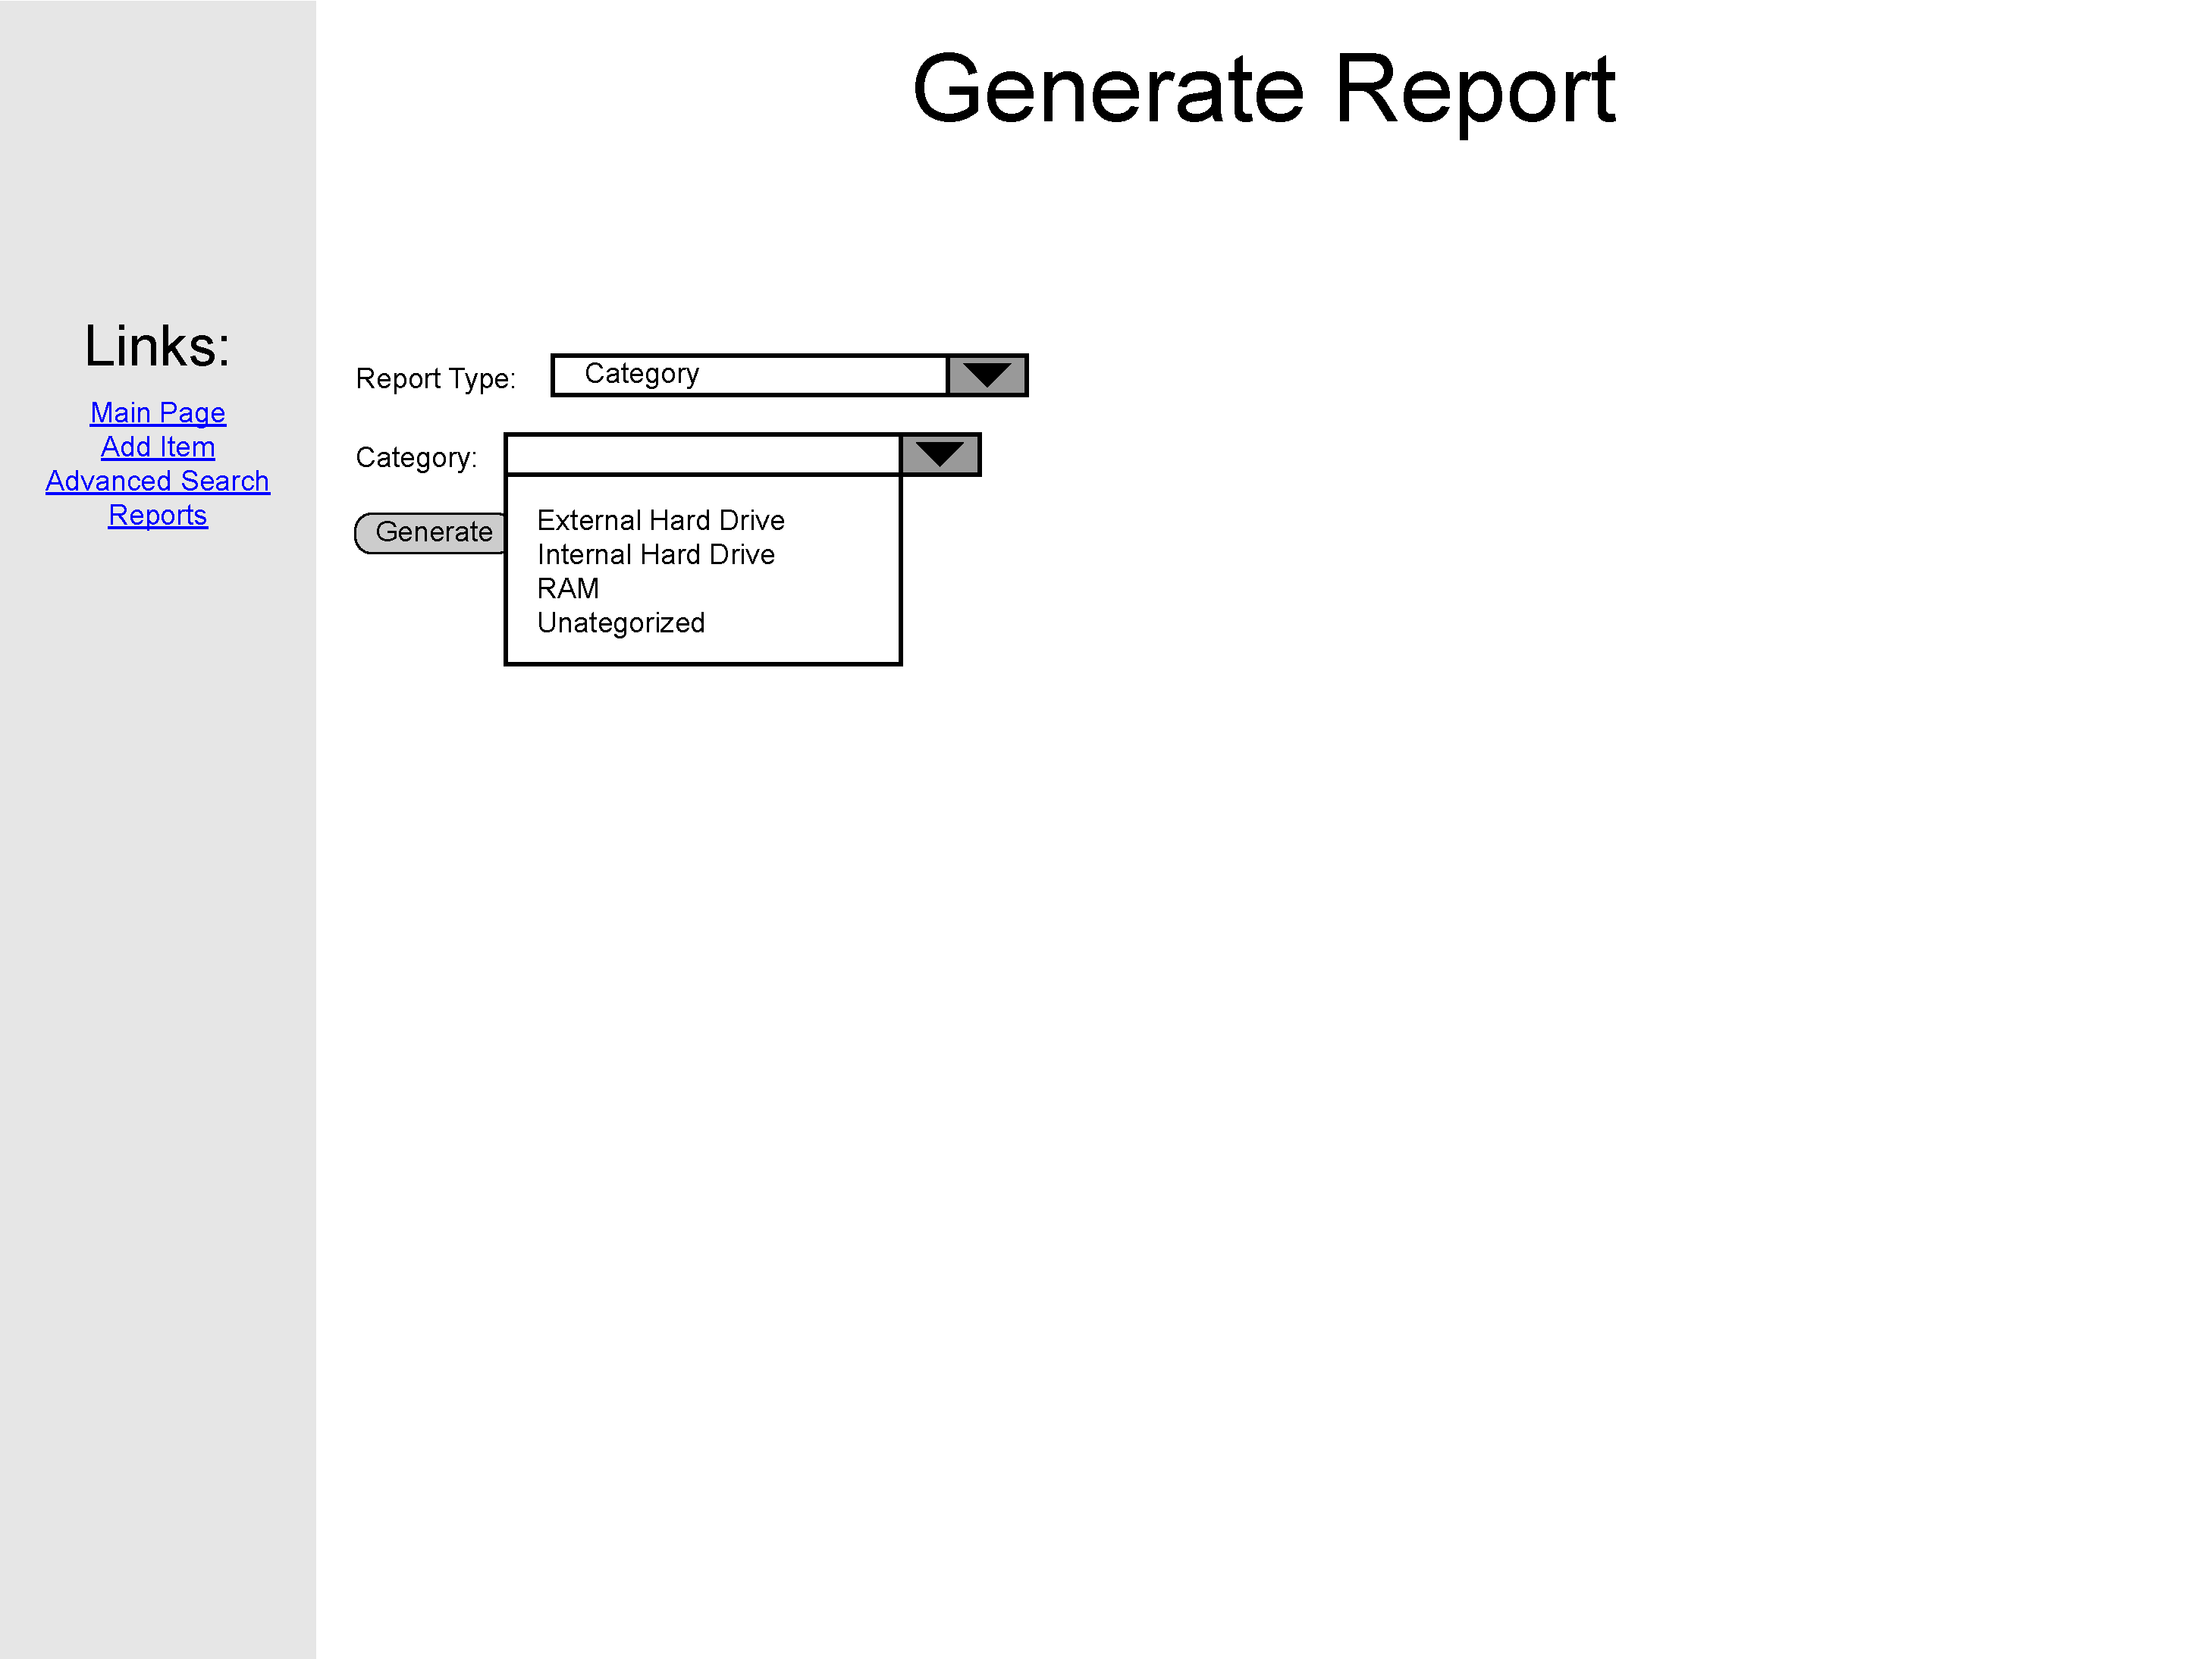
\includegraphics[keepaspectratio, width=4.5in]{generateReportF0S2.pdf} \\
The generate report page after the report type category has been selected, but before a category has been selected
\end{tabular}\\
~\\
~\\
\begin{tabular}{ p{4.5in} }
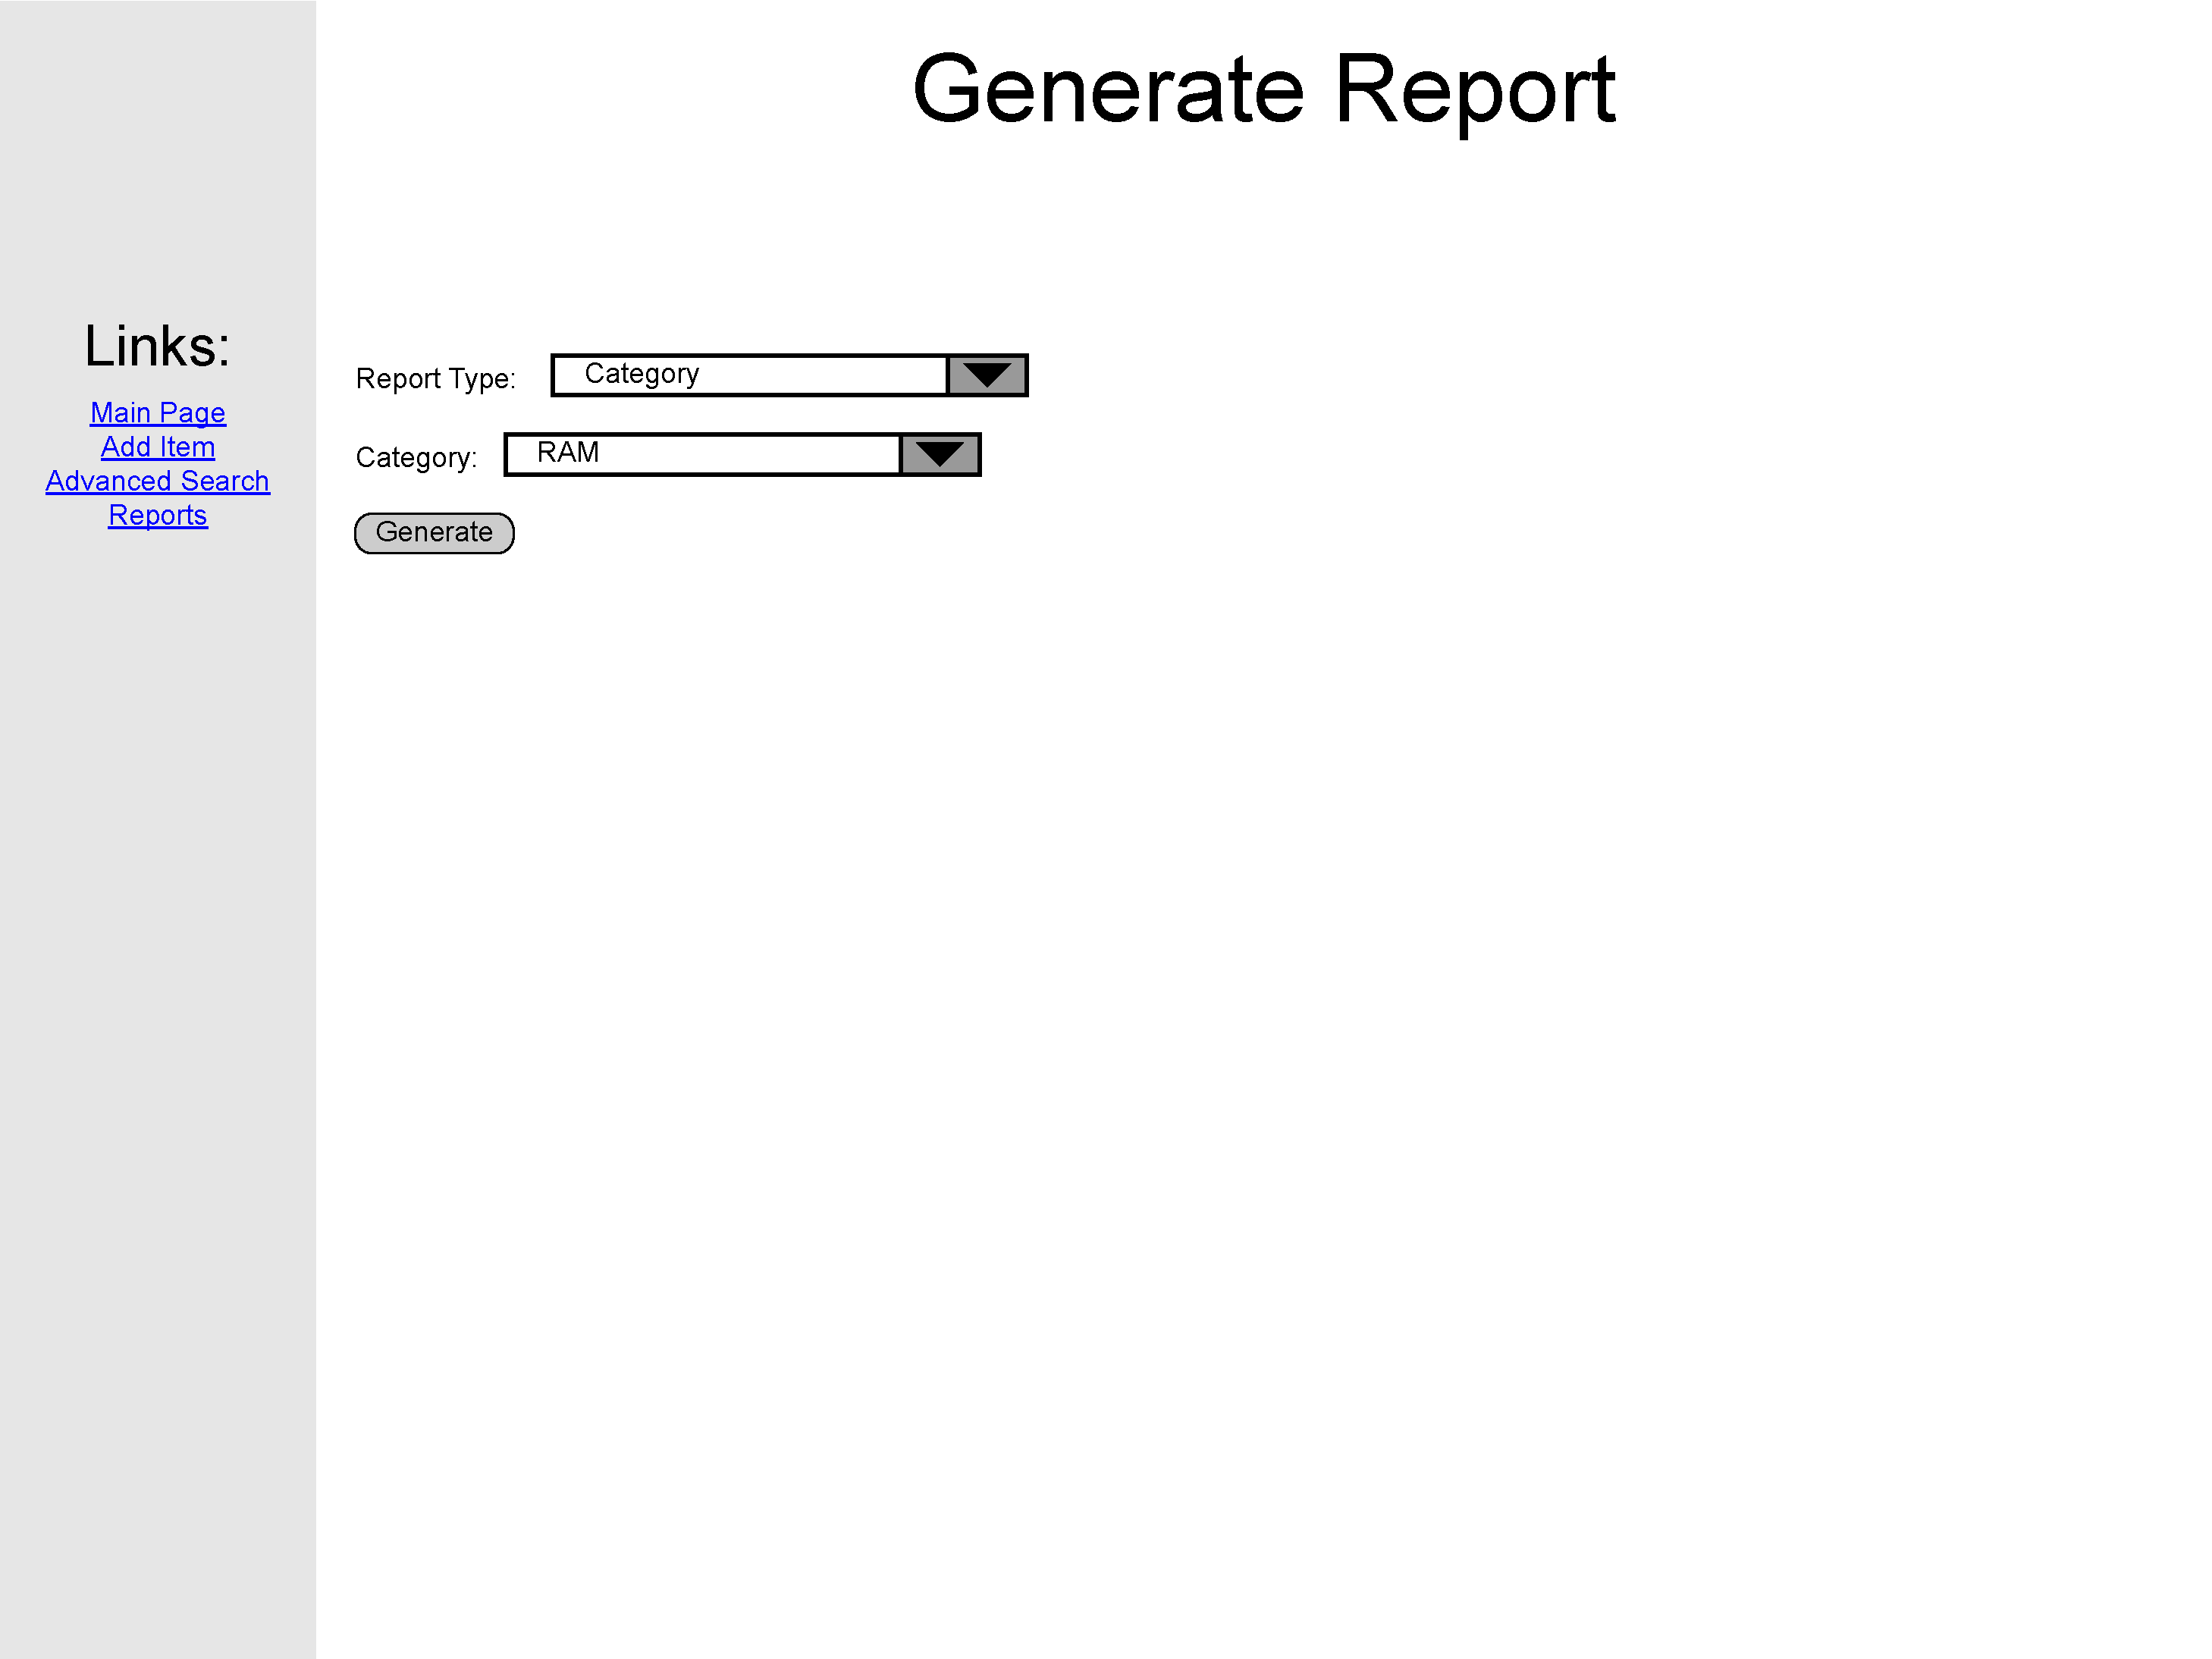
\includegraphics[keepaspectratio, width=4.5in]{generateReportF0S3.pdf} \\
The generate report page after the category of RAM has been selected
\end{tabular}\\
~\\
~\\
\begin{tabular}{ p{4.5in} }
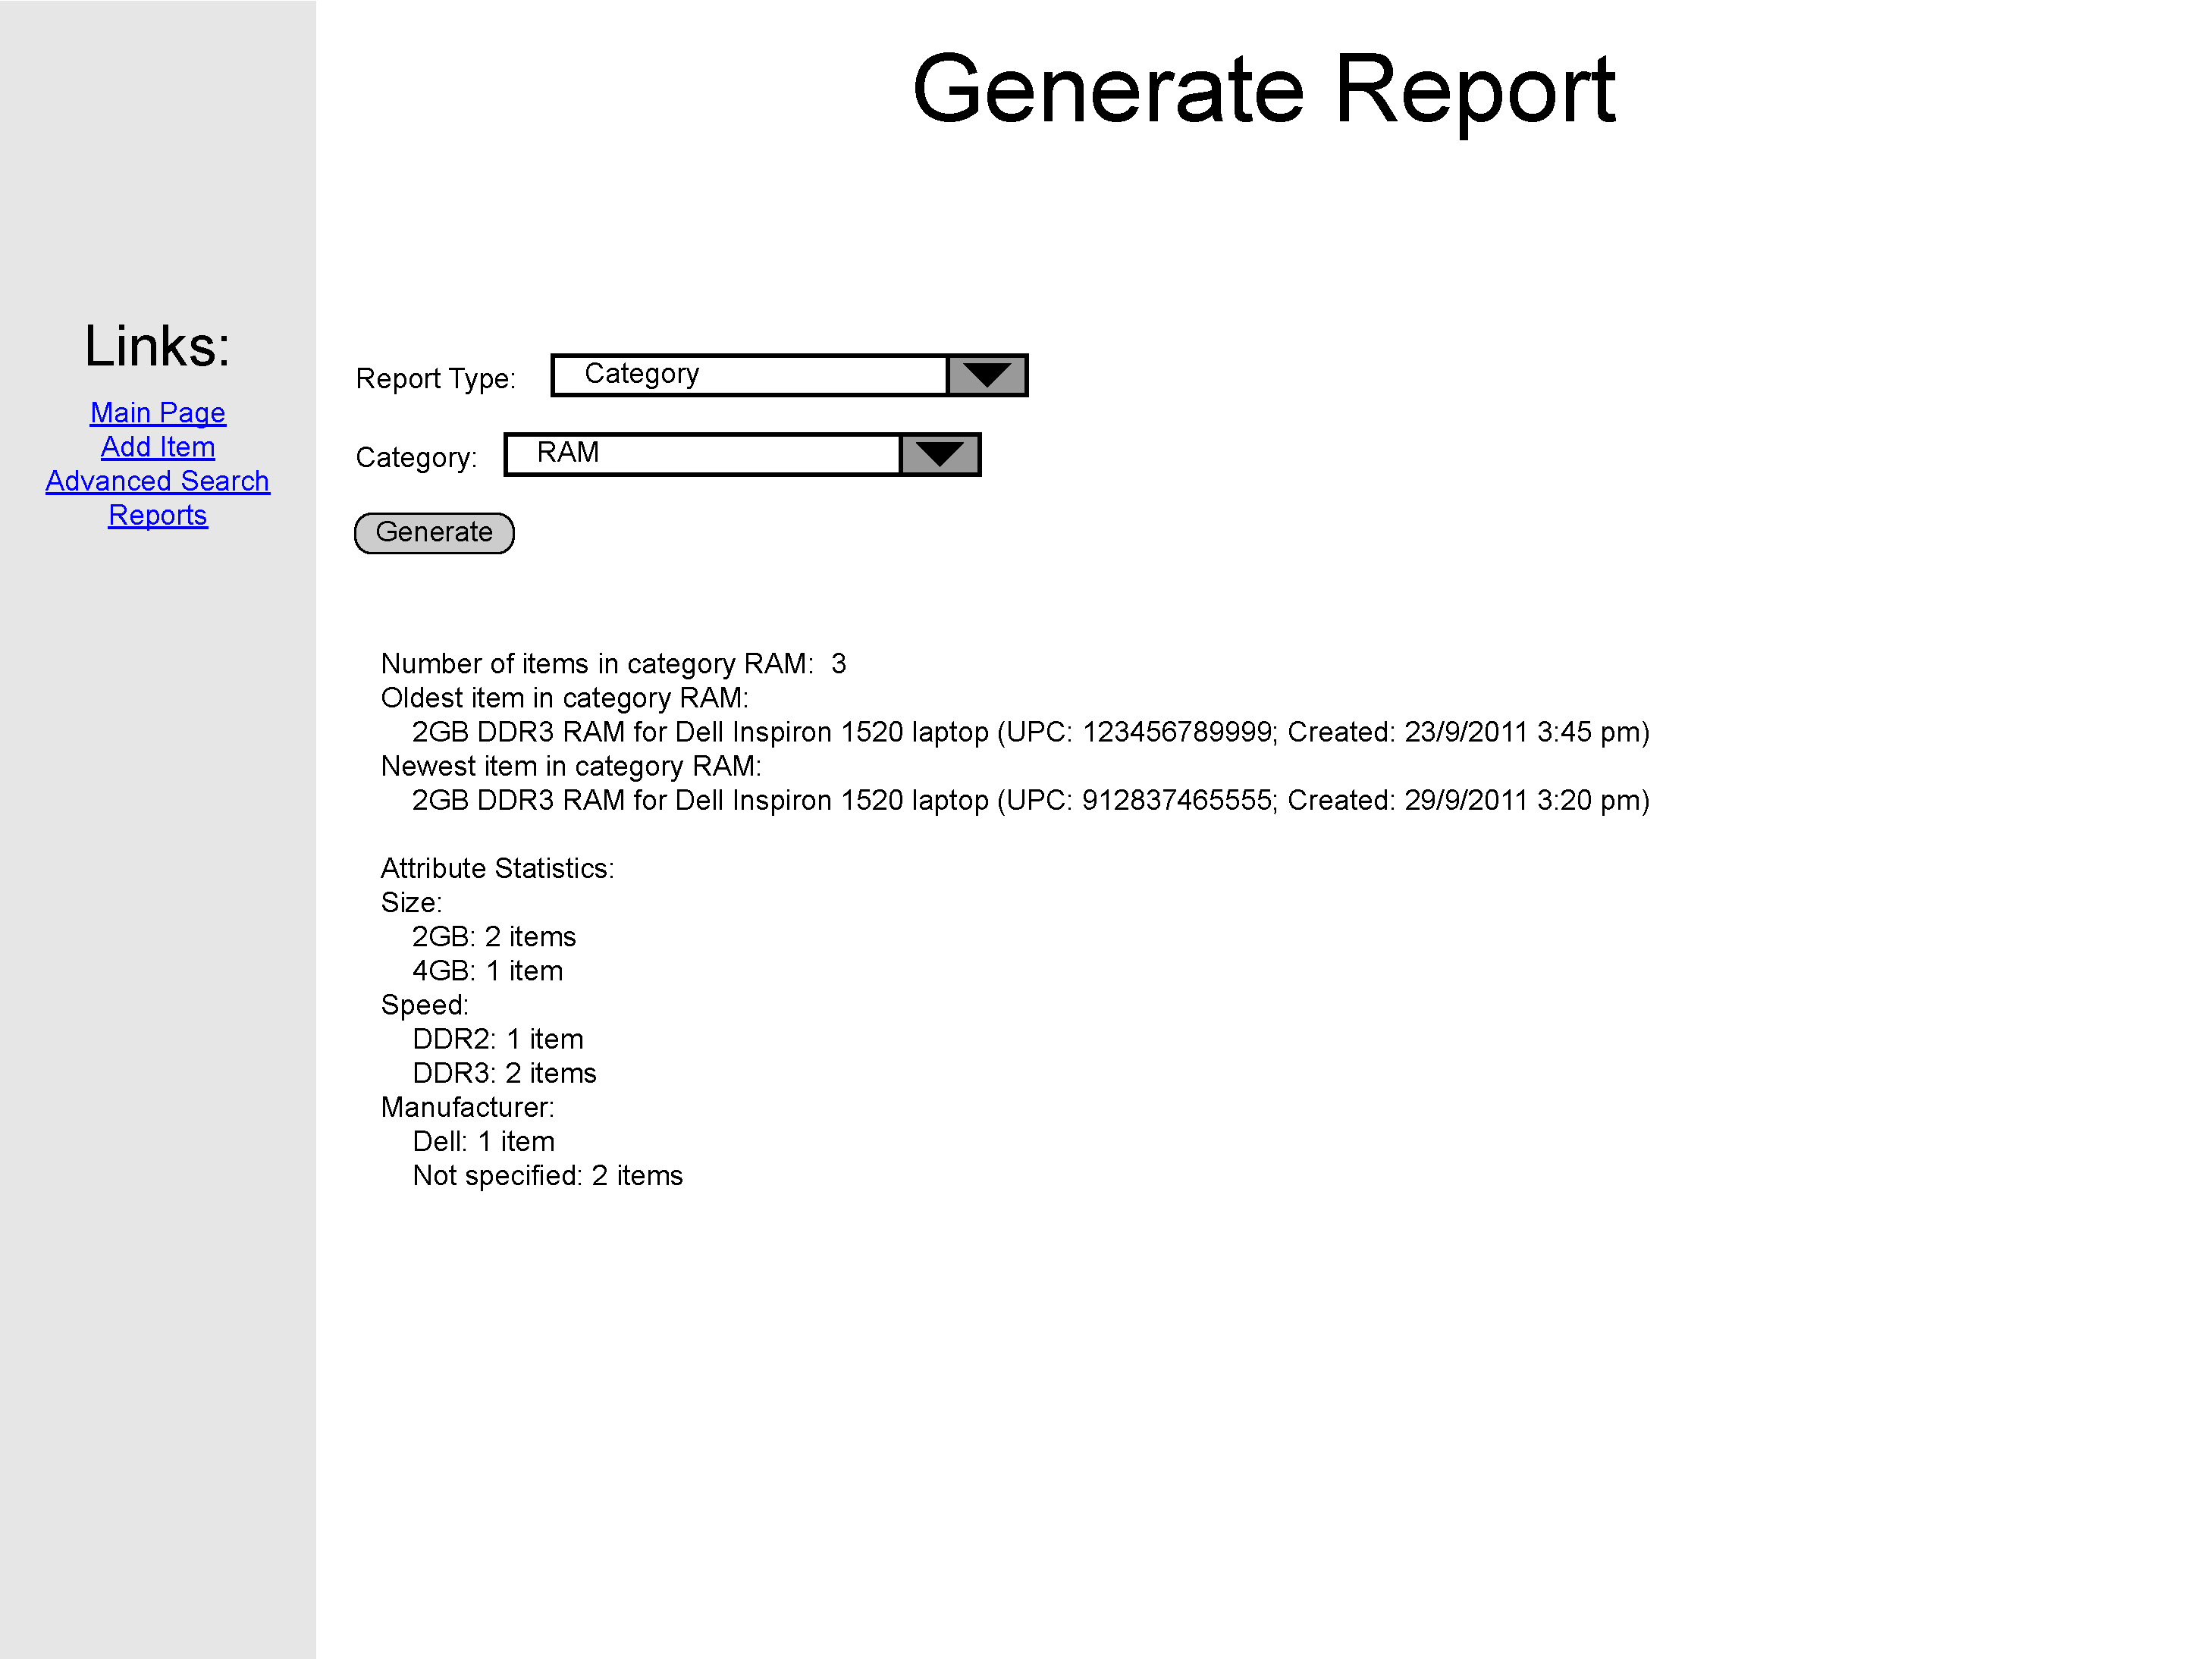
\includegraphics[keepaspectratio, width=4.5in]{generateReportF0S4.pdf} \\
The generate report page with the report being displayed
\end{tabular}

\section{Index and Glossary}

\section{References}
\hangindent=1.4cm
\textbf{(1)} Leffingwell, Dean, and Don Widrig.
\emph{Managing Software Requirements: a Use Case Approach}.
Addison-Wesley, Boston,
2nd Edition,
2003.\\

\noindent\hangindent=1.4cm
\textbf{(2)} ``Ruby 1.9.2''
\emph{Download Ruby.} Ruby. Web.  6 October 2011. \\

\noindent\hangindent=1.4cm
\textbf{(3)} ``Sinatra 1.3.0''
\emph{Sinatra: Documentation.} Sinatra. Web.  6 October 2011.\\

\noindent\hangindent=1.4cm
\textbf{(4)} ``Ubuntu 11.04''
\emph{Download Ubuntu.} Ubuntu. Web.  6 October 2011.\\

\noindent\hangindent=1.4cm
\textbf{(5)} ``SQLite 3.7.8''
\emph{SQLite Download Page.} SQLite. Web.  6 October 2011.\\

\noindent\hangindent=1.4cm
\textbf{(6)} ``Cucumber 1.1.0''
\emph{cucumber/cucumber.} Cucumber. Web.  6 October 2011.\\

\noindent\hangindent=1.4cm
\textbf{(7)} ``RSpec 2.6.0''
\emph{RSpec Documentation.} Relish. Web.  6 October 2011.\\

\noindent\hangindent=1.4cm
\textbf{(8)} ``DataMapper 1.1.0''
\emph{DataMapper - Documentation.} DataMapper. Web.  6 October 2011.\\

\noindent\hangindent=1.4cm
\textbf{(9)} ``Google Chrome 14.0.8'' 
\emph{About Google Chrome.} Google. Web.  7 October 2011.\\

\noindent\hangindent=1.4cm
\textbf{(10)} ``Firefox 7.0.1''
\emph{Mozilla Firefox Web Browser - Free Download.} Mozilla. Web.  7 October 2011.\\

\noindent\hangindent=1.4cm
\textbf{(11)} ``Apache 2.2''
\emph{Apache HTTP Server Version 2.2 Documentation - Apache HTTP Server.} Apache. Web.  7 October 2011.\\

\end{document}